\chapter{Cinématique des robots manipulateurs I: La position}
\label{sec:cine1}

Ce chapitre présente des méthodes pour modéliser et analyser la position de systèmes à plusieurs degrés de liberté, donc bien adaptés aux robots manipulateurs. Dans un contexte de robotique, les problèmes de cinématique consistent premièrement à bien choisir et définir des systèmes de coordonnées pertinents. Par exemple, des coordonnées généralisées pour décrire la configuration des joints, des coordonnées cartésiennes pour décrire la tâche d'un robot en terme de trajectoire de l'effecteur, des coordonnées sphériques pour décrire les mesures d'un système de vision, etc. Ensuite, le défi est de \textbf{calculer les fonctions de transformations pour passer d'un système de coordonnées à un autre}. Par exemple, pour les robots manipulateurs, le principal défi est le calcul de la fonction de la cinématique directe et son inverse, i.e. une fonction avec comme entrées les coordonnées généralisées qui représentent la configuration des joints et comme sortie la pose de l'effecteur. Le calcul de ces transformations dans un contexte de robotique est le sujet principal de ce chapitre. La section \ref{sec:syscoord} introduit aux différents systèmes de coordonnées. Les sections \ref{sec:vecgeopos} et \ref{sec:basevecpos} introduisent les notions de vecteurs de position géométriques, bases vectorielles et vecteur-colonnes de composantes. Les sections \ref{sec:changematrice} et \ref{sec:repere} présentent les changements de base et les changements des repères. Ensuite, la section \ref{sec:corps} présente les méthodes pour représenter mathématiquement la pose d'un corps rigide. Finalement, les sections \ref{sec:fwdkin} et \ref{sec:invkin} traitent de la cinématique des robots manipulateurs, i.e. le calcul des transformations pour passer de l'espace des joints à la pose de l'effecteur et vice-versa. 





%%%%%%%%%%%%%%%%%%%%%%%%%%%%%%%%%%%%%%%%%%%%%%%%%%%%%%%%%%%%%
\section{Systèmes de coordonnées}
\label{sec:syscoord}

Un système de coordonnées c'est un ensemble de scalaires, généralement des distances et des angles, qui décrivent la position d'un système. 

%%%%%%%%%%%%%%%%%%%%%%%%%%%%%%%%%%%%%%%%%%%%%%%%%%%
\subsection{Position d'une particule}
\label{sec:syscoordparticule}

Une particule (un point) dans l'espace tri-dimensionnel possède trois DDL et sa position peut donc être complètement déterminée par trois scalaires qui forment un système de coordonnées. Trois types de systèmes de coordonnées sont généralement utilisés pour décrire la position d'une particule par rapport à des axes: \textbf{cartésien} $( x, y, z)$, \textbf{cylindrique} $( r, \theta, z)$ ou \textbf{sphérique} $( \rho, \theta, \phi)$, voir la figure \ref{fig:coorsys}. 

%%%%%%%%%%%%%%%%%%%%%%%%%%%%%%%%%%%%%%%%%%%%%%%%%%%%%%%%%%%%%%%
\begin{figure}[H]
				%\vspace{-10pt}
        \centering
        \subfloat[Cartésien]{
				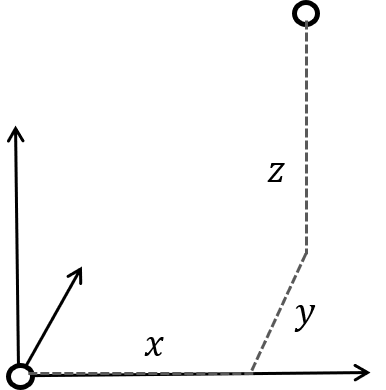
\includegraphics[width=0.28\textwidth]{carsys}
				\label{fig:carsys}}
				\subfloat[Cylindrique]{
				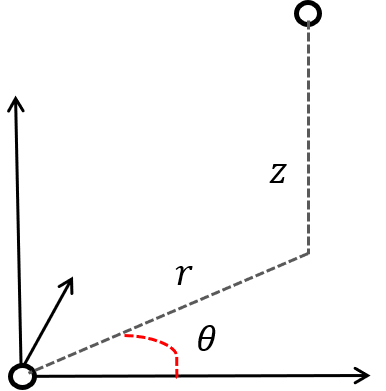
\includegraphics[width=0.28\textwidth]{cylsys}
				\label{fig:cylsys}}
				\subfloat[Sphérique]{
				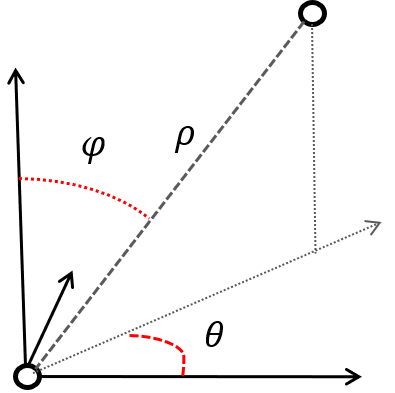
\includegraphics[width=0.28\textwidth]{sphsys}
				\label{fig:sphsys}}
        \caption{Trois systèmes de coordonnées standards pour représenter la position d'un point en 3D}
				\label{fig:coorsys}
\end{figure}
%%%%%%%%%%%%%%%%%%%%%%%%%%%%%%%%%%%%%%%%%%%%%%%%%%%%%%%%%%%%%%%%%

Selon la situation, l'utilisation d'un système de coordonnées particulier peut simplifier l'analyse d'un problème. Par exemple, pour localiser un point géographique sur la Terre, des coordonnées sphériques (ex.: longitude et latitude) sont plus pratiques que des coordonnées cartésiennes ($x$,$y$,$z$) par rapport au centre de la Terre. Parfois l'utilisation d'un type de système de coordonnées est nécessaire car un capteur mesure une coordonnée particulière. Par exemple, le \textit{LIDAR} sur une voiture autonome mesure des distances dans plusieurs directions grâce à un laser pivotant, les données brute sont des coordonnées sphériques. Il est donc parfois inévitable de faire la conversion d'un système de coordonnées à un autre. Le tableau \ref{tab:convcoord} donne les conversions entre des coordonnées cartésiennes, cylindriques et sphériques, qui sont basées sur la même origine et le même système d'axes.
%%%%%%%%%%%%%%%%%%%%%%%%%%%
\begin{table}[htbp]
	\centering
		\begin{tabular}{|p{3cm}|p{3cm}|p{3cm}|p{3cm}|}
		\hline
		 & De cartésien & De cylindrique & De sphérique \\
		\hline 
		 Vers cartésien &
			\vbox{\begin{align*}
			x &= x \\
			y &= y \\
			z &= z
			\end{align*}} 
			& 
			% Polaire vers xyz
			\vbox{\begin{align*}
			x &= r \cos \theta \\
			y &= r \sin \theta \\
			z &= z
			\end{align*}}
			& 
			% Spherical vers xyz
			\vbox{\begin{align*}
			x &= \rho \sin \phi \cos \theta \\
			y &= \rho \sin \phi \sin \theta \\
			z &= \rho \cos \phi
			\end{align*}}
			\\
		\hline
		  Vers cylindrique &
			% xyz vers cylindrique
			\vbox{\begin{align*}
			r &= \sqrt{x^2+y^2} \\
			\theta &= \arctan \frac{y}{x} \\
			z &= z
			\end{align*}}
			&  %cylindrique vers cylindrique
			\vbox{\begin{align*}
			r &= r \\
			\theta &= \theta \\
			z &= z
			\end{align*}}
			& %spherique vers cylindrique
			\vbox{\begin{align*}
			r &= \rho \sin \phi \\
			\theta &= \theta \\
			z &= \rho \cos \phi
			\end{align*}}
			\\
		\hline
		  Vers sphérique &
			% xyz vers Spherical 
			\vbox{\begin{align*}
			\rho &= \sqrt{x^2+y^2+z^2} \\
			\theta &= \arctan \frac{y}{x} \\
			\phi &= \arctan \frac{\sqrt{x^2+y^2}}{z}
			\end{align*}}
			& 
			% cylindrical vers Spherical 
			\vbox{\begin{align*}
			\rho &= \sqrt{r^2+z^2} \\
			\theta &= \theta \\
			\phi &= \arctan \frac{r}{z}
			\end{align*}}
			& 
			%  Spherical 
			\vbox{\begin{align*}
			\rho &= \rho \\
			\theta &= \theta \\
			\phi &= \phi
			\end{align*}}
			\\
		\hline
		\end{tabular}
	\caption{Conversions entre les systèmes de coordonnées cartésiennes, polaires et sphériques qui font référence aux même axes et à la même origine.}
	\label{tab:convcoord}
\end{table}
%%%%%%%%%%%%%%%%%%%%%%%%%%%%%%%%

%%%%%%%%%%%%%%%%%%%%%%%%%%%%%%%%%%%%%%%%%%%
\subsection{Pose d'un corps rigide}
\label{sec:syscoordpose}

Pour décrire la position d'un corps rigide, trois scalaires qui représentent l'orientation sont nécessaires en plus des trois coordonnées qui spécifient la translation, pour un total de six DDL. La combinaison de la translation et de l'orientation est souvent appelée \textbf{la pose} d'un objet. La translation est typiquement spécifiée par la position d'un point sur le corps rigide (ex.: son centre) avec les différentes représentations discutées à la section \ref{sec:syscoordparticule} (cartésienne, cylindrique ou sphérique) et l'orientation est typiquement spécifiée par trois angles. Comme illustré à la figure \ref{fig:pose}, les six coordonnées suivantes pourraient être utilisées pour spécifier la pose d'un objet:
%%%%%%%%%%%%%
\begin{align}
\text{La translation (3 DDL), ex.:} \quad &\left[ x, y, z \right] \\
\text{L'orientation (3 DDL), ex.:} \quad &\left[ \theta_{tangage}, \theta_{roulis}, \theta_{lacet} \right]
\end{align}
%%%%%%%%%%%%%
Il est à noter que \textbf{la représentation de l'orientation d'un corps rigide est un problème complexe} et qu'il existe plusieurs méthodes alternatives pour représenter l'orientation (matrices de rotations, angles de Euler, représentation axe-angle, quaternions, etc.) qui seront discutées à la section \ref{sec:corps}. Selon les domaines (robotique, aérospatiale, engins graphiques des jeux vidéos, vision par ordinateur, astronomie, etc.), différents standards et conventions existent en terme de coordonnées utilisées pour décrire l'orientation. Le point à retenir pour le moment est que trois coordonnées indépendantes sont nécessaires pour représenter une orientation arbitraire, donc six totales sont nécessaires pour représenter une pose arbitraire. Par exemple, un minimum de six coordonnées doivent être utilisées pour: spécifier la position de l'effecteur d'un robot, décrire la position d'un avion dans le ciel, décrire la position de la terre par rapport au soleil, etc. 

\begin{figure}[htbp]
	\centering
		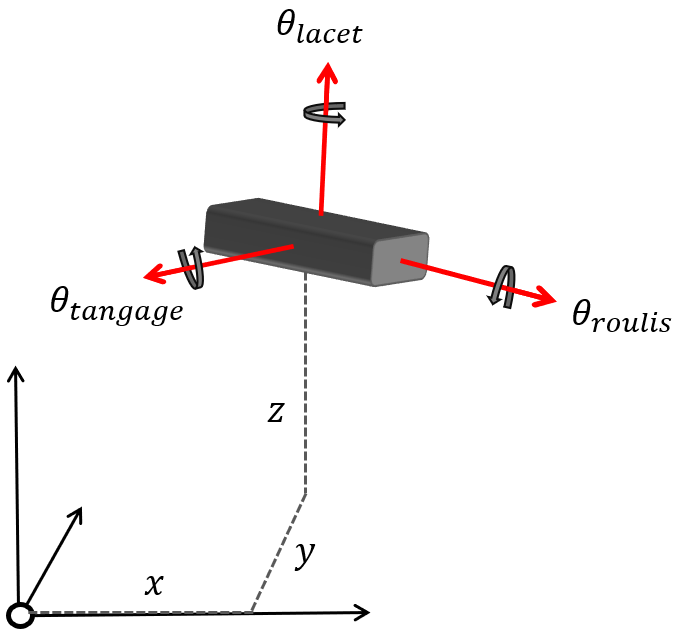
\includegraphics[width=0.50\textwidth]{pose.png}
	\caption{Six coordonnées sont nécessaire pour représenter la pose d'un corps rigide, trois pour décrire la translation et trois pour décrire son orientation.}
	\label{fig:pose}
\end{figure}


%%%%%%%%%%%%%%%%%%%%%%%%%%%%%%%%%%%%%%%%%%%%%%%%%%%%%%
\subsection{Configuration d'un robot manipulateur}
Pour représenter la configuration d'un robot manipulateur il faut suffisamment de variables pour décrire la position relative de chacun des liens rigides qui le compose. Le choix des coordonnées doit être adapté à la géométrie du robot étudié. Un ensemble de variables indépendantes, généralement des angles et des distances, qui permet de déterminer la configuration d'un robot est appelé \textbf{coordonnées généralisées}. L'adjectif \textit{généralisées} est historique et a ici le sens de \textit{pas nécessairement cartésiennes}. Le nombre de coordonnées généralisées nécessaire correspond au nombre de \textbf{degrés-de-liberté} (DDL) du robot.
%\paragraph{Exemples de coordonnées généralisées}
La figure \ref{fig:coor} montre trois exemples de deux coordonnées indépendantes qui peuvent être utilisées comme coordonnées généralisées pour décrire la configuration d'un robot à deux joints rotatifs.

%%%%%%%%%%%%%%%%%%%%%%%%%%%%%%%%%%%%%%%%%%%%%%%%%%%%%%%%%%%%%%%
\begin{figure}[htbp]
				%\vspace{-10pt}
        \centering
        \subfloat[Deux angles relatifs]{
				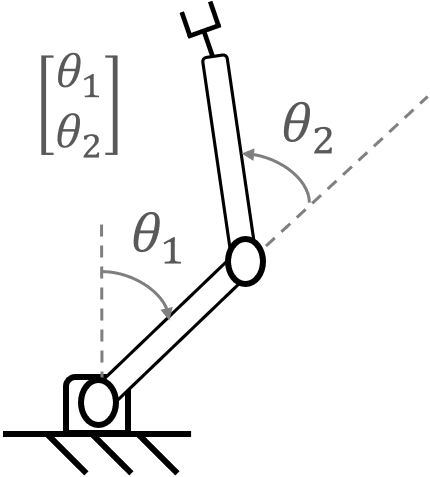
\includegraphics[width=0.24\textwidth]{coor_theta}
				\label{fig:coor_theta}}
				\vspace{10pt}
				\subfloat[Deux angles absolus]{
				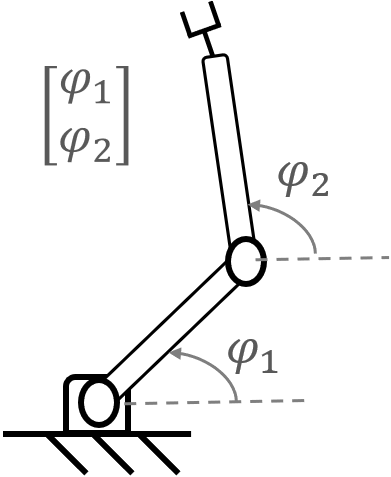
\includegraphics[width=0.22\textwidth]{coor_phi}
				\label{fig:coor_phi}}
				\vspace{10pt}
				\subfloat[Deux distances]{
				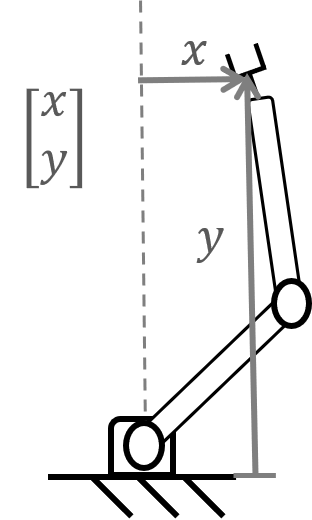
\includegraphics[width=0.18\textwidth]{coor_xy}
				\label{fig:coor_xy}}
				\vspace{-10pt}
        \caption{Trois possibilités de coordonnées indépendantes pour spécifier la position d'un robot à 2 DDL}
				\label{fig:coor}
\end{figure}
%%%%%%%%%%%%%%%%%%%%%%%%%%%%%%%%%%%%%%%%%%%%%%%%%%%%%%%%%%%%%%%%%

%\subsubsection{Espace des joints et espace de la tâche}

\subsubsection{Deux types de systèmes de coordonnées sont généralement utilisés en robotique:}

\paragraph{Espace des joints/actionneurs}

Pour les robots manipulateurs, les algorithmes de contrôle utilisent généralement des coordonnées généralisées qui correspondent à des mesures du déplacement relatif de chaque joint comme illustré à la figure \ref{fig:jointspace}. Ces coordonnées sont généralement notées $\col{q} = \left[ \begin{array}{cccc} q_1 & q_2 & ... & q_n \end{array} \right]^T$ (où $n$ est le nombre de DDL) et on réfère aussi à ce système comme \textbf{l'espace des joints}. Chaque coordonnée $q_i$ représente alors une mesure locale du DDL qui relie deux liens rigides séquentiels. Pour les robots industriels par exemple, ce système de coordonnées est très utile car des encodeurs mesurent directement ces variables et les moteurs les contrôlent de façon indépendante. 

\paragraph{Espace de la tâche}

La tâche d'un robot peut rarement être spécifiée facilement dans l'espace des joints. Un système de coordonnées naturel pour la tâche doit donc généralement être utilisé et on réfère aussi à ce système comme \textbf{l'espace de la tâche}. La tâche d'un robot manipulateur est généralement spécifiée plus naturellement en termes de coordonnées cartésiennes de l'effecteur. Il est à noter que le nombre de coordonnées nécessaires pour l'espace de la tâche peut être différent du nombre de DDL total du robot. Comme illustré à la figure \ref{fig:taskspace}, pour un robot qui aurait comme tâche d'écrire sur une plaque, l'objectif serait naturellement exprimé par une trajectoire définie avec des coordonnées $(x,y)$ sur la plaque. 

%%%%%%%%%%%%%%%%%%%%%%%%%%%%%%%%%%%%%%%%%%%%%%%%%%%%%%%%%%%%%%%
\begin{figure}[htbp]
				%\vspace{-10pt}
        \centering
        \subfloat[Espace des joints]{
				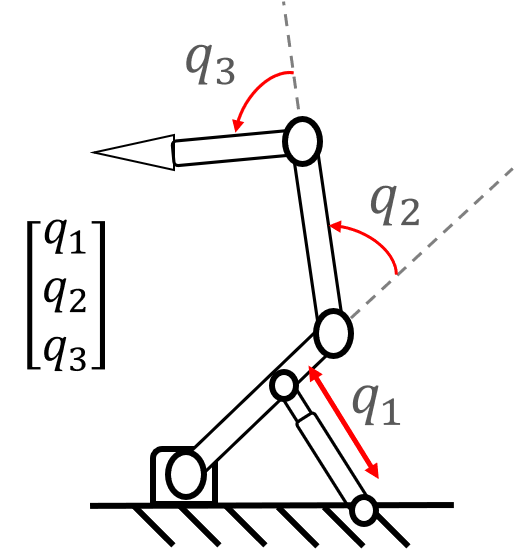
\includegraphics[width=0.28\textwidth]{jointspace}
				\label{fig:jointspace}}
				\hspace{+20pt}
				\subfloat[Espace de la tache]{
				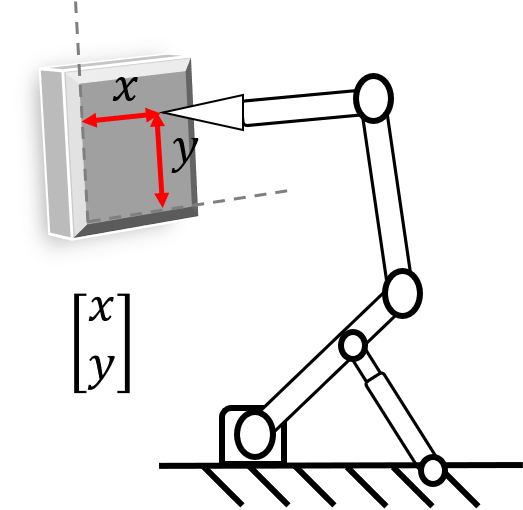
\includegraphics[width=0.28\textwidth]{taskspace}
				\label{fig:taskspace}}
        \caption{Exemple de coordonnées représentant l'espace des joints et l'espace tâche d'un robot manipulateur}
				\label{fig:spaces}
\end{figure}
%%%%%%%%%%%%%%%%%%%%%%%%%%%%%%%%%%%%%%%%%%%%%%%%%%%%%%%%%%%%%%%%%


\section{L'approche présentée dans ce chapitre}

L'approche de modélisation mise de l'avant dans ce chapitre, et illustrée à la Figure \ref{fig:approchemodelisation}, ce résume à la séquence:
\begin{enumerate}
	\item Décrire le problème avec des vecteurs géométriques symboliques;
	\item Choisir des bases appropriées;
	\item Traduire la relation vectorielle en relation matricielle (projection dans une base);
	\item Déterminer la solution numérique avec les outils de l'algèbre linéaire.
\end{enumerate}
%%%%%%%%%%%%%%%%%%%%%%%%%%%%%%%%%%%%%%%%%%
\begin{figure}[H]
	\centering
		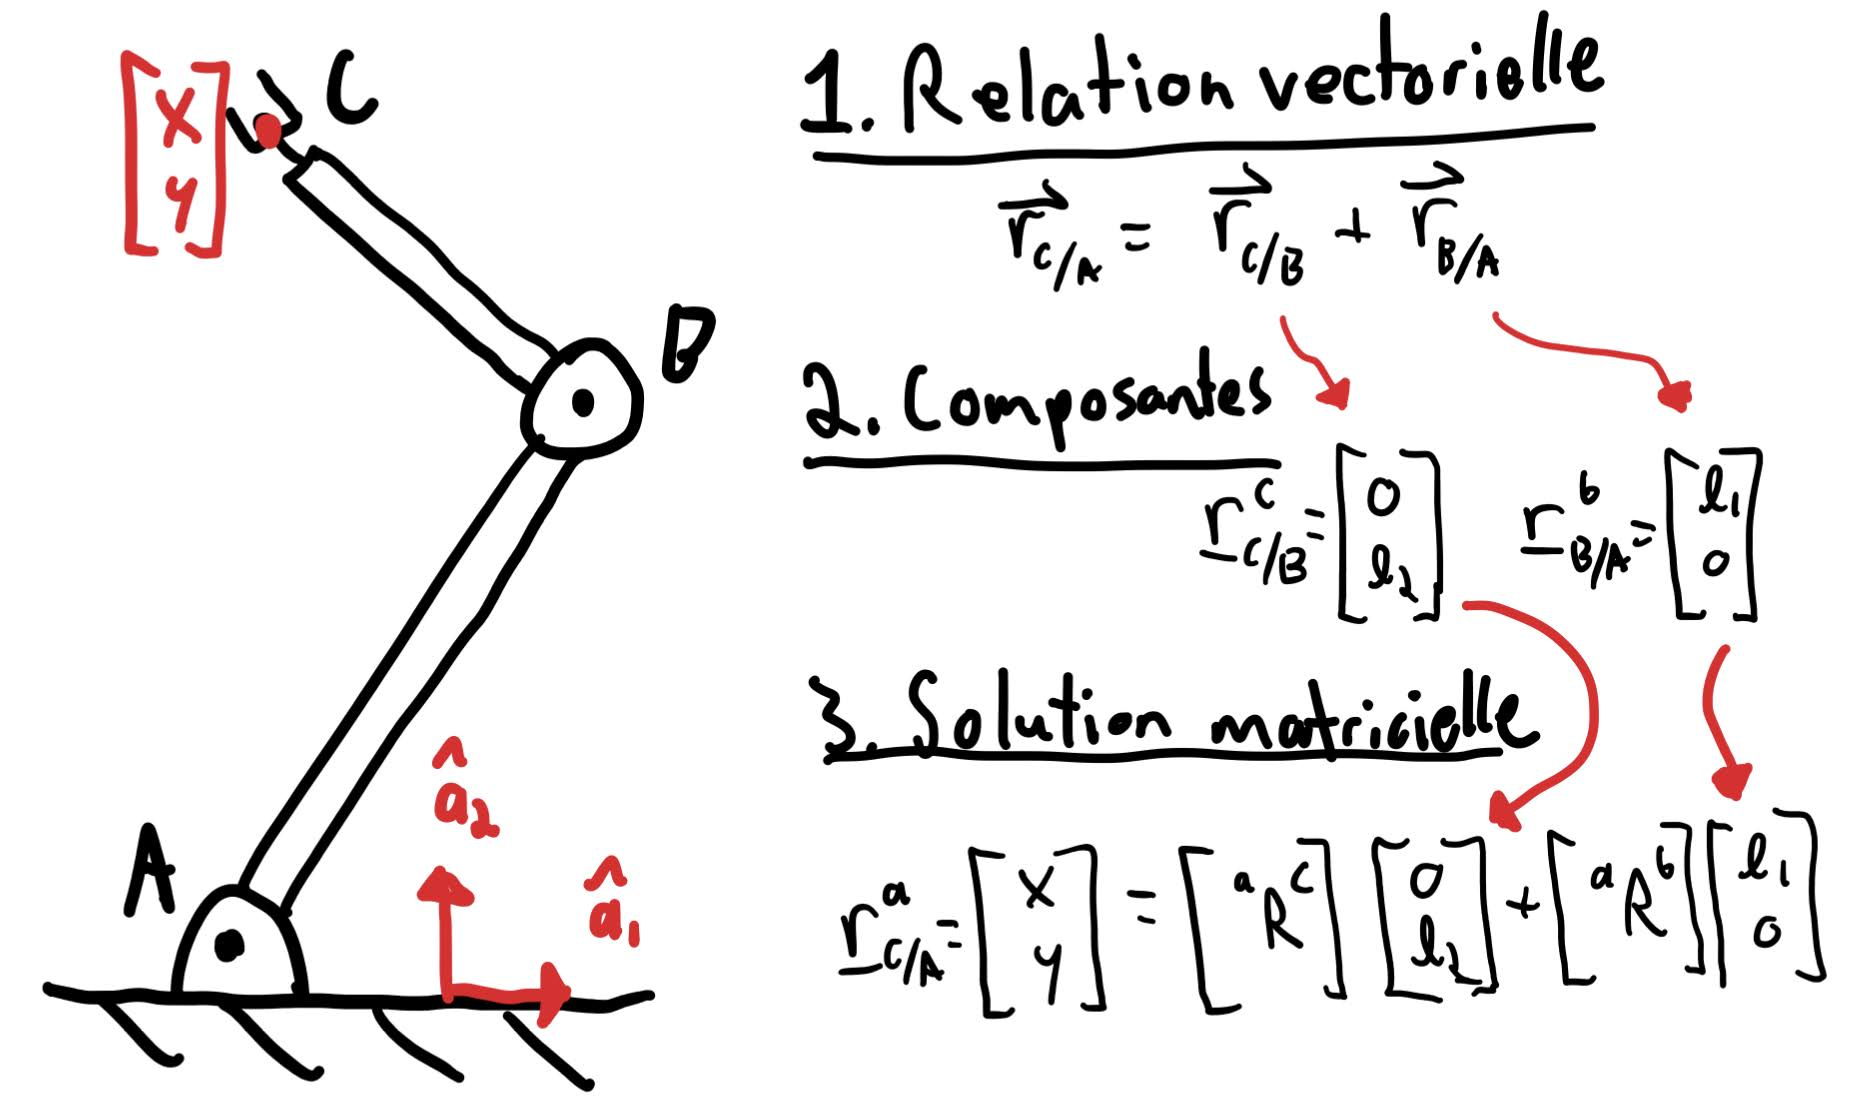
\includegraphics[width=0.7\textwidth]{approchemodelisation.jpg}
	\caption{Aperçu des grandes lignes de l'approche de modélisation présentée dans ces notes}
	\label{fig:approchemodelisation}
\end{figure}
%%%%%%%%%%%%%%%%%%%%%%%%%%%%%%%%%%%%%%%%%%
  



%%%%%%%%%%%%%%%%%%%%%%%%%%%%%%%%%%%%%%%%%%%%%%%%%%%%%%%%%%%%%%%%%%%%%%%%%%%%%%%%%%%%%%%%%%%%%%%%%%%%%%%%%%%%%%%%%%%%%%%%%%%%%%%%%%
\newpage
\section{Vecteurs géométriques de positions}
\label{sec:vecgeopos}

La notion de vecteur géométrique permet de travailler avec des \textbf{vecteurs de position} qui sont indépendants d'un choix de système de coordonnées. Pour les problèmes de cinématique de robots, il est particulièrement adapté de travailler d'abord avec les vecteurs géométrique, plutôt que directement avec des coordonnées. Cette approche \textbf{1)} simplifie les calculs en 3D et \textbf{2)} permet de faire le saut facilement entre plusieurs systèmes de coordonnées. Un vecteur géométrique est une quantité définie dans l’espace et possédant une grandeur et une direction. Dans ces notes, les vecteurs géométriques, notés $\vec{v}$, seront explicitement distingués des vecteur-colonnes (groupe de plusieurs scalaires) qui seront notés $\col{v}=\left[  \begin{array}{ccc} v_{1} & v_{2} & v_{3} \end{array} \right]^T$, voir chapitre \ref{sec:calcvec}.

\video{Les vecteurs géométrique de position}{https://youtu.be/5DeO4NeFAO8}
%\subsubsection{Vecteurs de positions}

\textbf{Un vecteur position nécessite deux points pour être défini}, une origine et une destination. Notez que c'est particulier des vecteurs positions, la plupart des autres vecteurs utilisés en physique (vitesse, accélération, force, champ électrique, etc.) ont un point d'application mais sont indépendants d'un choix d’origine. Dans ces notes, les vecteurs positions seront notés:
%%%%%%%%%%%%%%%%%%%%%%%%%%%%%%%%%%%
\begin{equation}
\vec{r}_{B/A}  \quad =  \quad \text{Vecteur position du point $B$ par rapport au point $A$}
\end{equation} 
%%%%%%%%%%%%%%%%%%%%%%%%%%%%%%%%%%%
où $A$ est le point d'origine et $B$ le point de destination, tel qu'illustré à la figure \ref{fig:vecpos}. Parfois, la notation équivalente $\vec{AB}$ est utilisée dans la littérature. Ces vecteurs  peuvent être utilisés pour faire des constructions géométriques indépendamment d'un choix de système de coordonnées. 
%
%%%%%%%%%%%%%%%%%%%%%%%%%%%%%%%%%%%%%%%%%%%%%%%%%%%%%%%%%%%%%%%
\begin{figure}[htb]
				%\vspace{-10pt}
        \centering
				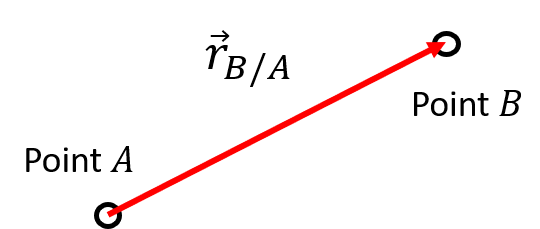
\includegraphics[width=0.30\textwidth]{vecpos}
				\caption{Un vecteur position}
        %\subfloat[Un Vecteur Positions]{
				%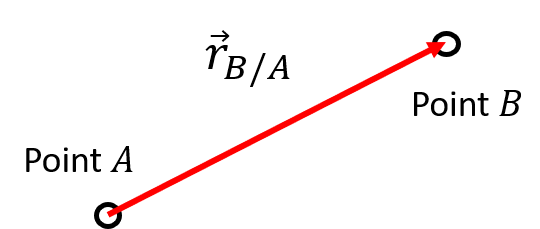
\includegraphics[width=0.30\textwidth]{vecpos}
				%\label{fig:vecpos}}
				%\subfloat[Construction géométrique]{
				%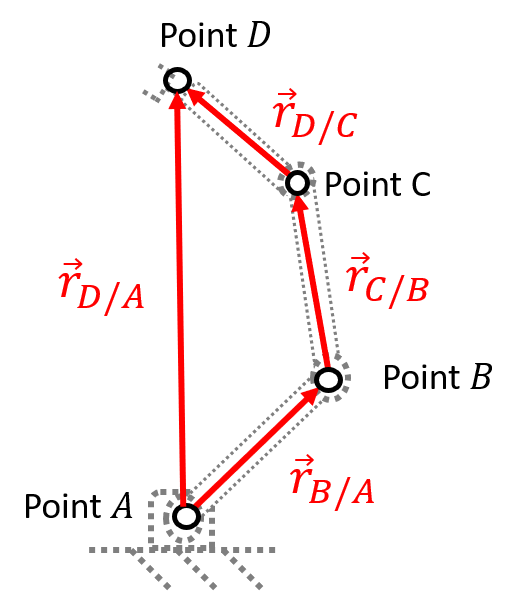
\includegraphics[width=0.30\textwidth]{vecposcons}
				%\label{fig:vecposcons}}
        %\caption{Example de vecteurs de position}
				\label{fig:vecpos}
\end{figure}
%%%%%%%%%%%%%%%%%%%%%%%%%%%%%%%%%%%%%%%%%%%%%%%%%%%%%%%%%%%%%%%%%
%

%%%%%%%%%%%%%%%%%%%%%%%%%%%%%%%%%%%%%%%%%%%%%%%
\subsection{Propriétés des vecteurs de position}
\label{sec:vecposprop}
%
La figure \ref{fig:vecposprop} illustre les propriétés de base des vecteurs de position.
%
%%%%%%%%%%%%%%%%%%%%%%%%%%%%%%%%%%%%%%%%%%%%%%%%%%%%%%%%%%%%%%%
\begin{figure}[htbp]
				%\vspace{-10pt}
        \centering
        \subfloat[Inversion]{
				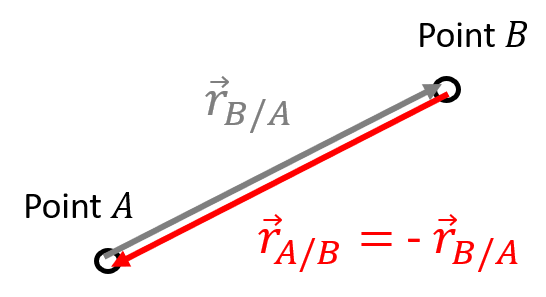
\includegraphics[width=0.28\textwidth]{vecposinv}
				\label{fig:vecposinv}}
				\hspace{5pt}
				\subfloat[Vecteur unitaire et distance]{
				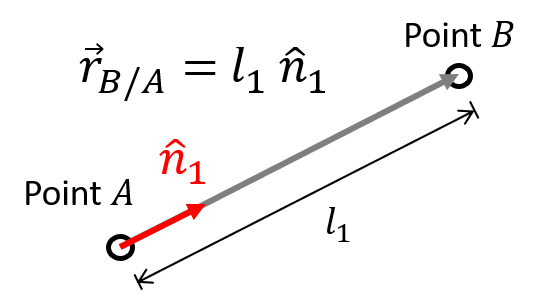
\includegraphics[width=0.28\textwidth]{vecposvecuni}
				\label{fig:vecposinv}}
				\hspace{5pt}
				\subfloat[Addition]{
				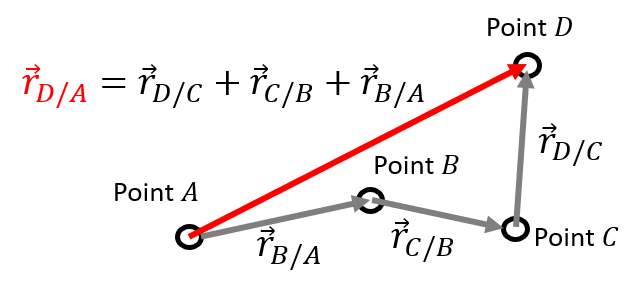
\includegraphics[width=0.35\textwidth]{vecposadd}
				\label{fig:vecposinv}}
				%\vspace{-10pt}
        \caption{Propiétés des vecteurs de position}
				\label{fig:vecposprop}
\end{figure}
%%%%%%%%%%%%%%%%%%%%%%%%%%%%%%%%%%%%%%%%%%%%%%%%%%%%%%%%%%%%%%%%%
%
% \paragraph{Addition}
\begin{property}[Addition]
%
Un vecteur position peut être décomposé en une addition de vecteurs qui passent par des points intermédiaires:
%%%%%%%%%%%%%%%%%%%%%%%%%%%%%%%%%%%
\begin{align}
\vec{r}_{Z/A}  =   \vec{r}_{Z/Y} + \vec{r}_{Y/X} + ... + \vec{r}_{C/B} + \vec{r}_{B/A} 
\end{align} 
%%%%%%%%%%%%%%%%%%%%%%%%%%%%%%%%%%%
\end{property}
%
\begin{property}[Inversion]
%
L'inversion de l'origine et la destination est équivalente à la négation du vecteur de position:
%%%%%%%%%%%%%%%%%%%%%%%%%%%%%%%%%%%
\begin{align}
\vec{r}_{B/A}  = - \vec{r}_{A/B}
\end{align} 
%%%%%%%%%%%%%%%%%%%%%%%%%%%%%%%%%%%
\end{property}
%
\begin{property}[Vecteurs unitaires]
%
Les vecteurs positions peuvent être exprimés comme des \textbf{combinaisons de distances et directions} qui sont représentées respectivement par des paires de scalaires $l_i$ et vecteurs unitaires $\hat{n}_i$ (qui représente des directions dans l'espace):
%%%%%%%%%%%%%%%%%%%%%%%%%%%%%%%%%%%
\begin{equation}
\vec{r} = l_1 \hat{n}_1 + l_2 \hat{n}_2 + ... + l_n \hat{n}_n
\end{equation} 
%%%%%%%%%%%%%%%%%%%%%%%%%%%%%%%%%%%
\end{property}



\begin{property}[Norme]
La norme d'un vecteur position, i.e. sa longueur, peut être calculée en effectuant un produit scalaire du vecteur avec lui même:
%%%%%%%%%%%%%%%%%%%%%%%%%%%%%%%%%%%
\begin{equation}
\| \vec{r} \|^2 = \vec{r} \bullet \vec{r} 
\label{eq:dotnorm}
\end{equation} 
%%%%%%%%%%%%%%%%%%%%%%%%%%%%%%%%%%%
\end{property}

\begin{property}[Projection]
La longueur $d$ d'un vecteur position $\vec{r}$ projeté selon un axe particulier correspond au produit scalaire du vecteur position avec un vecteur unitaire $\hat{n}$ aligné sur cet axe:
%%%%%%%%%%%%%%%%%%%%%%%%%%%%%%%%%%%
\begin{equation}
d = \vec{r} \bullet \hat{n} = \| \vec{r} \|  \cos \angle (\vec{r},\hat{n})
\label{eq:vecproj}
\end{equation} 
%%%%%%%%%%%%%%%%%%%%%%%%%%%%%%%%%%%
Cette opération est aussi appelée \textbf{projection d'un vecteur sur un axe} et illustrée à la figure \ref{fig:distproj}. 
\end{property}

\begin{property}[Angle]
Le produit scalaire de deux vecteurs unitaires est égale au cosinus de l'angle qui les sépare puisqu'ils ont une dimension unitaire:
%%%%%%%%%%%%%%%%%%%%%%%%%%%%%%%%%%%
\begin{equation}
\cos \angle (\hat{n}_1,\hat{n}_2) =  \hat{n}_1 \bullet \hat{n}_2
\label{eq:dotangle}
\end{equation} 
%%%%%%%%%%%%%%%%%%%%%%%%%%%%%%%%%%%
Il est donc possible d'utiliser le produit scalaire pour mesurer un angle entre deux vecteurs, comme illustré à la figure \ref{fig:dotcosuni}.  
\end{property}
%
%%%%%%%%%%%%%%%%%%%%%%%%%%%%%%%%%%%%%%%%%%%%%%%%%%%%%%%%%%%%%%%
\begin{figure}[htbp]
				%\vspace{-10pt}
        \centering
        \subfloat[Distance selon un axe]{
				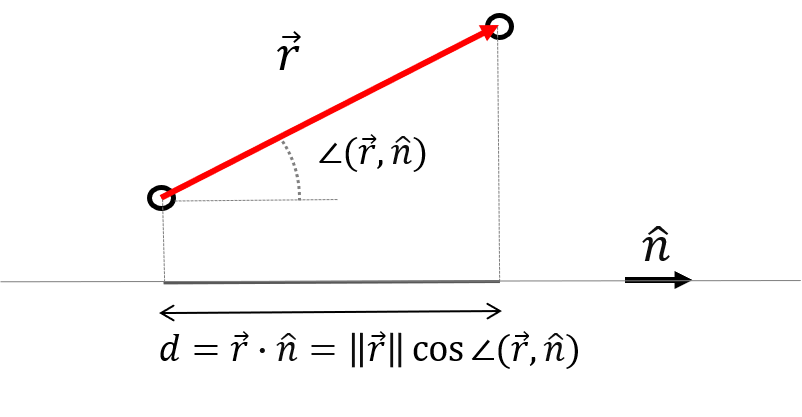
\includegraphics[width=0.40\textwidth]{distproj}
				\label{fig:distproj}}
				\hspace{20pt}
				\subfloat[Angle entre deux vecteurs unitaires]{
				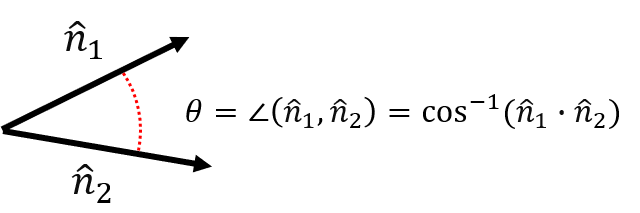
\includegraphics[width=0.35\textwidth]{dotcosuni}
				\label{fig:dotcosuni}}
        \caption{Utilisation du produit scalaire pour des mesures géométriques}
				\label{fig:utprosca}
\end{figure}
%%%%%%%%%%%%%%%%%%%%%%%%%%%%%%%%%%%%%%%%%%%%%%%%%%%%%%%%%%%%%%%%%
%TODO ajouter figure pour la norme

\video{Exemple de calcul avec les vecteurs géométrique de position}{https://youtu.be/YqmyBJPJmP0}


\begin{example}[Calcul de la hauteur d'un robot]
\label{sec:hauteurrobot}

Un exemple est ici donné pour le calcul de la hauteur de l'effecteur d'un robot à 3 DDL, illustré à la figure \ref{fig:vecposphi}, avec l'aide des vecteurs géométriques de position. Comme illustré à la Figure \ref{fig:vecposcons}, par inspection il est possible de déterminer la relation vectorielle suivante:
%%%%%%%%%%%%%%%%%%%%%%%%%%%%%%%%%%%
\begin{equation}
\vec{r}_{D/A} = \vec{r}_{D/C} + \vec{r}_{C/B} + \vec{r}_{B/A}
\label{eq:vecadd}
\end{equation} 
%%%%%%%%%%%%%%%%%%%%%%%%%%%%%%%%%%%
Ensuite, comme illustré à la figure \ref{fig:vecposuni}, des vecteurs unitaires $\hat{n}_i$ alignés avec chacun des liens rigides du robot manipulateur permettent de préciser l'équation \eqref{eq:vecadd} avec des longueurs et des directions:
%%%%%%%%%%%%%%%%%%%%%%%%%%%%%%%%%%%
\begin{equation}
\vec{r}_{D/A} = l_1 \hat{n}_{1} + l_2 \hat{n}_{2} + l_3 \hat{n}_{3}
\label{eq:vecadduni}
\end{equation} 
%%%%%%%%%%%%%%%%%%%%%%%%%%%%%%%%%%%
Finalement, pour calculer la hauteur $h$ de ce robot par exemple, il suffit de prendre le produit scalaire avec un vecteur unitaire vertical $\hat{y}$:
%%%%%%%%%%%%%%%%%%%%%%%%%%%%%%%%%%%
\begin{align}
h &= \vec{r}_{D/A} \bullet \hat{y} \\
h &= ( l_1 \hat{n}_{1} + l_2 \hat{n}_{2} + l_3 \hat{n}_{3} ) \bullet \hat{y} \\
h &= l_1 ( \hat{n}_{1} \bullet \hat{y} ) + l_2 ( \hat{n}_{2} \bullet \hat{y} ) + l_3 ( \hat{n}_{3}  \bullet \hat{y} ) \\
h &= l_1 \cos \angle (\hat{n}_{1},\hat{y}) + l_2 \cos \angle (\hat{n}_{2},\hat{y}) + l_3 \cos \angle (\hat{n}_{3},\hat{y})
\label{eq:vecaddproj}
\end{align} 
%%%%%%%%%%%%%%%%%%%%%%%%%%%%%%%%%%%
À noter ici que le produit scalaire de deux vecteurs unitaires correspond au cosinus de l'angle entre les deux vecteurs, voir équation \eqref{eq:dotangle}. Donc avec l’exemple ci-dessus le produit scalaire $\hat{n}_{i} \bullet \hat{y}$ correspond simplement au cosinus de l'angle du joint $i$ avec l'axe vertical, donné par les angles $\varphi_i$ à la figure \ref{fig:vecposphi}. L'équation \eqref{eq:vecaddproj} peut donc être précisée comme une expression des variables de distances $l_i$ et des variables d'angles $\varphi_i$: 
%%%%%%%%%%%%%%%%%%%%%%%%%%%%%%%%%%%
\begin{align}
h &= l_1 \cos (\varphi_1) + l_2 \cos (\varphi_2) + l_3 \cos (\varphi_3)
\label{eq:vecaddprojphi}
\end{align} 
%%%%%%%%%%%%%%%%%%%%%%%%%%%%%%%%%%%
Dans un cas simple planaire comme celui-ci il aurait été assez simple de calculer la hauteur du robot directement par trigonométrie. L'approche vectorielle est toutefois plus systématique et se généralise beaucoup plus facilement à des systèmes complexes et tri-dimensionnels comme les robots industriels.
%
%%%%%%%%%%%%%%%%%%%%%%%%%%%%%%%%%%%%%%%%%%%%%%%%%%%%%%%%%%%%%%%
\begin{figure}[H]
				%\vspace{-10pt}
        \centering
				%%%
        \subfloat[Robot à 3 DLL]{
				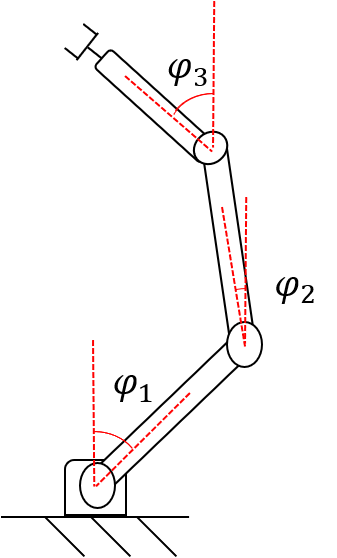
\includegraphics[width=0.17\textwidth]{vecposphi}
				\label{fig:vecposphi}}
				%%%%%%%%%%%%%%%%%%
				\hspace{3pt}
				%%%%
				\subfloat[Vecteurs géométrique]{
				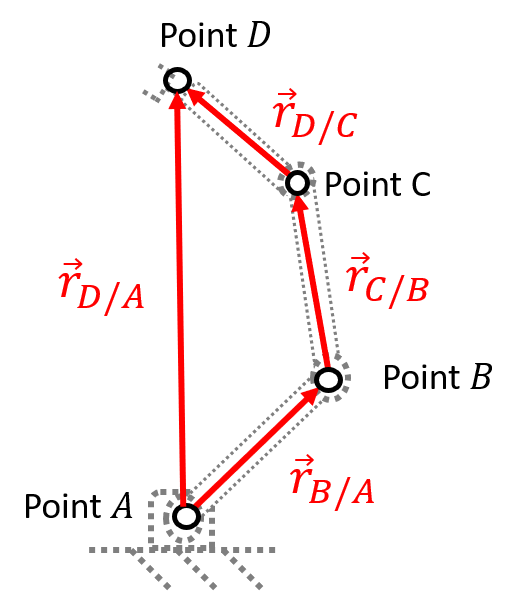
\includegraphics[width=0.26\textwidth]{vecposcons}
				\label{fig:vecposcons}}
				%%%%
				\hspace{3pt}
				%%%%
        \subfloat[Vecteur unitaires]{
				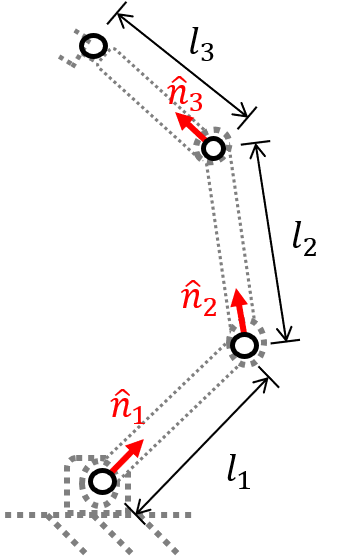
\includegraphics[width=0.17\textwidth]{vecposuni}
				\label{fig:vecposuni}}
				%%%%
				\hspace{3pt}
				%%%%
				\subfloat[Projection sur l'axe vertical]{
				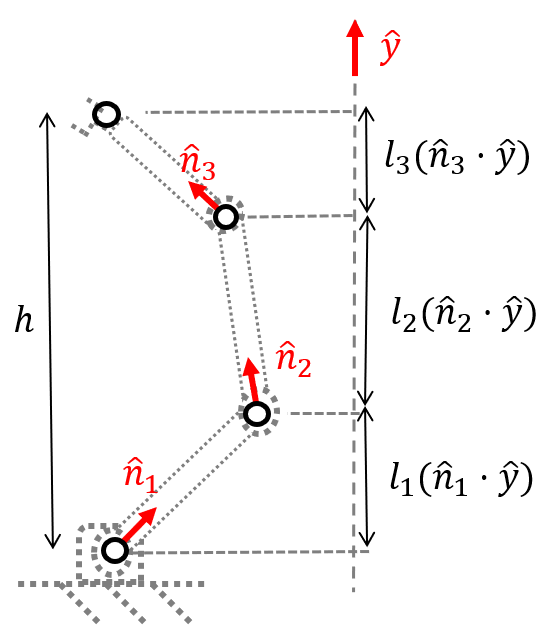
\includegraphics[width=0.29\textwidth]{vecpospro}
				\label{fig:vecpospro}}
        \caption{Exemple de calcul de la hauteur d'un robot.}
				\label{fig:vecposunipro}
\end{figure}
%%%%%%%%%%%%%%%%%%%%%%%%%%%%%%%%%%%%%%%%%%%%%%%%%%%%%%%%%%%%%%%
\end{example}

%TODO, faire exemple 3D vectoriel ici


\subsection{Procédure d'utilisation pour le calcul de distances}
La démarche utilisée pour calculer des positions avec les vecteurs géométriques se résume par les trois étapes suivantes:
\begin{enumerate}
	\item Par inspection, construire le vecteur position $\vec{r}$ d’intérêt comme une addition/soustraction de plusieurs vecteurs positions $\vec{r}_i$ avec des longueurs et orientations connues:
	%%%%%%%%%%%%%%%%%%%%%%%%%%%%%%%%%%%
	\begin{equation}
	\vec{r} = \sum_i \vec{r}_i
	\end{equation} 
	%%%%%%%%%%%%%%%%%%%%%%%%%%%%%%%%%%%
	\item Substituer les vecteurs positions symboliques $\vec{r}_i$ par des variables de distance $l_i$ et des vecteurs unitaires $\hat{n}_i$ représentant des directions qui peuvent être mesurées:
	%%%%%%%%%%%%%%%%%%%%%%%%%%%%%%%%%%%
	\begin{equation}
	\vec{r} = \sum_i l_i \hat{n}_i
	\end{equation} 
	%%%%%%%%%%%%%%%%%%%%%%%%%%%%%%%%%%%
	\item Calculer les distances désirées $d$ en effectuant un produit scalaire avec les vecteurs unitaires selon les axes désirés:
	%%%%%%%%%%%%%%%%%%%%%%%%%%%%%%%%%%%
	\begin{align}
	d_x = \vec{r} \bullet \hat{x} = \sum_i l_i ( \hat{n}_i \bullet \hat{x} ) =  \sum_i l_i \cos \angle (\hat{n}_{i},\hat{x}) \\ 
	d_y = \vec{r} \bullet \hat{y} = \sum_i l_i ( \hat{n}_i \bullet \hat{y} ) =  \sum_i l_i \cos \angle (\hat{n}_{i},\hat{y}) \\ 
	d_z = \vec{r} \bullet \hat{z} = \sum_i l_i ( \hat{n}_i \bullet \hat{z} ) =  \sum_i l_i \cos \angle (\hat{n}_{i},\hat{z}) 
	\end{align} 
	%%%%%%%%%%%%%%%%%%%%%%%%%%%%%%%%%%%
\end{enumerate}



%%%%%%%%%%%%%%%%%%%%%%%%%%%%%%%%%%%%%%%%%%%%%%%%%%%%%%%%%%%%%%%%%%%%%%%%%%%%%%%%%%%%%%%%%%%%%%%%%%%%%%%%%%%%%%%%%%%%%%%%%%%%%%
\newpage
\section{Bases vectorielles et composantes d'un vecteur position}
\label{sec:basevecpos}

Les vecteurs positions tri-dimensionnels $\vec{r}$ peuvent être décris par trois scalaires qui représentent des distances ($r_1$, $r_2$ et $r_3$) qui multiplient trois vecteur unitaires orthogonaux ($\hat{a}_1$, $\hat{a}_2$ et $\hat{a}_3$) qui forment une base vectorielle.  Les scalaires $r_i$ qui multiplient chaque vecteur unitaire sont appelés composantes et peuvent être regroupés sous la forme d'un vecteur-colonne, la notation suivante sera utilisée:
%%%%%%%%%%%%%%%%%%%%%%%%%%%%%%%%%%%
\begin{equation}
\text{\textbf{Vecteur-géométrique:}}\quad
\vec{r} = r_1^a \, \hat{a}_{1} + r_2^a \, \hat{a}_{2} + r_3^a \, \hat{a}_{3}
\quad \quad 
\text{\textbf{Vecteur-colonne:}}\quad
\col{r}^{a} = \left[ \begin{array}{c} r_1^a \\ r_2^a \\ r_3^a  \end{array} \right] 
\label{eq:veccoldef}
\end{equation} 
%%%%%%%%%%%%%%%%%%%%%%%%%%%%%%%%%%%
où l'exposant $a$ est utilisé pour spécifier la base vectorielle associée aux composantes scalaires. 


% %%%%%%%%%%%%%%%%%%%%%%%%%%%%%%%%%%%%%%%%%%%%%%%%%%%%%%%%%%%%%%%
% \begin{figure}[htpb]
% 				%\vspace{-10pt}
%         \centering
% 				\subfloat[Base $a$]{
% 				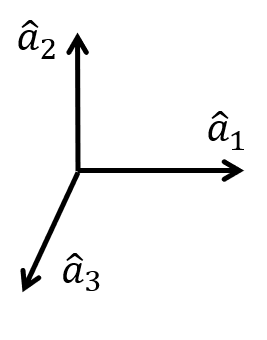
\includegraphics[width=0.20\textwidth]{base}
% 				\label{fig:base}}
% 				%%%%
% 				\hspace{10pt}
% 				%%%%
%         \subfloat[Vecteur vs. ses composantes]{
% 				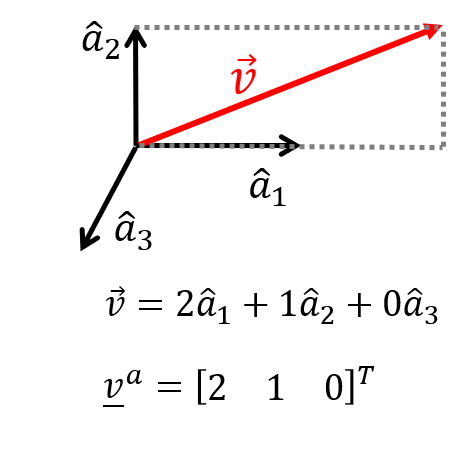
\includegraphics[width=0.25\textwidth]{baseex}
% 				\label{fig:baseex}}
% 				%%%%
% 				\hspace{10pt}
% 				%%%%
% 				\subfloat[Convention de la main droite]{
% 				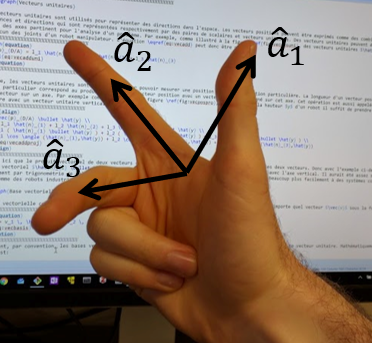
\includegraphics[width=0.25\textwidth]{righthand}
% 				\label{fig:righthand}}
%         \caption{Les bases vectorielles}
% 				\label{fig:vecbasis}
% \end{figure}
% %%%%%%%%%%%%%%%%%%%%%%%%%%%%%%%%%%%%%%%%%%%%%%%%%%%%%%%%%%%%%%%%%

%%%%%%%%%%%%%%%%%%%%%%%%%%%%%%%%%%%%%%%%%%%%%%%%%%%%%%%%%%%%%%%%%
\note{Note sur la séquence de lecture: }{Il est suggérer au lecteur de lire les sections \ref{sec:vec}, \ref{vectorbasis} et \ref{sec:opeveccol} dans le chapitre \ref{sec:calcvec} qui couvre le calcul vectoriel de façon plus générique. Ces sections couvrent plus en détails les fondements qui sont ici utilisés dans un contexte de cinématique. }
%%%%%%%%%%%%%%%%%%%%%%%%%%%%%%%%%%%%%%%%%%%%%%%%%%%%%%%%%%%%%%%%%

\video{Les bases vectorielles et composantes d'un vecteur}{https://youtu.be/pZdoFz5PpKU}

%%%%%%%%%%%%%%%%%%%%%%%%%%%%%%%%%%%%%%%%%%
\subsection{Rappel sur les bases vectorielles}
\label{vectorbasisrap}
Une base vectorielle correspond à un ensemble de trois vecteurs unitaires (en 3D) orthogonaux qui déterminent l'orientation de trois axes dans l'espace et forment une base qui permet de décrire n'importe quel vecteur position $\vec{r}$ sous la forme:
%%%%%%%%%%%%%%%%%%%%%%%%%%%%%%%%%%%
\begin{equation}
\vec{r} = r_1^a \, \hat{a}_{1} + r_2^a \, \hat{a}_{2} + r_3^a \, \hat{a}_{3}
\label{eq:vecbasisr}
\end{equation} 
%%%%%%%%%%%%%%%%%%%%%%%%%%%%%%%%%%%
On appellera \textit{base vectorielle} $a$, une base formée par l'ensemble des vecteurs unitaires $\{\hat{a}_{1},\hat{a}_{2},\hat{a}_{3}\}$.
%
%%%%%%%%%%%%%%%%%%%%%%%%%%%%%%%%%%%%%%%%%%%%%%%%%%%%%%%%%%%%%%%
\begin{figure}[htpb]
				%\vspace{-10pt}
        \centering
				\subfloat[Base $a$]{
				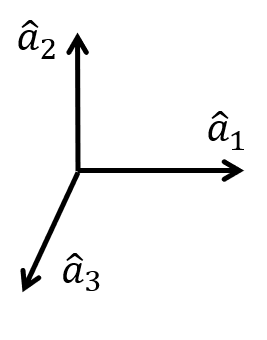
\includegraphics[width=0.20\textwidth]{base}
				\label{fig:base}}
				%%%%
				\hspace{10pt}
				%%%%
        \subfloat[Exemple]{
				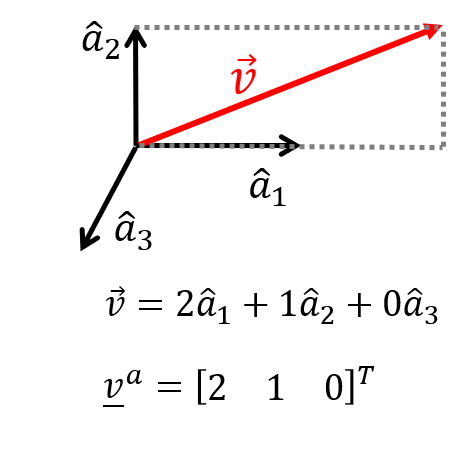
\includegraphics[width=0.25\textwidth]{baseex}
				\label{fig:baseex}}
				%%%%
				\hspace{10pt}
				%%%%
				\subfloat[Convention de la main droite]{
				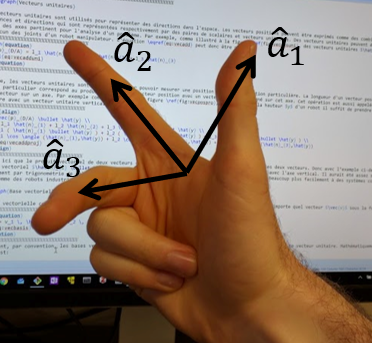
\includegraphics[width=0.25\textwidth]{righthand}
				\label{fig:righthand}}
        \caption{Les bases vectorielles}
				\label{fig:vecbasis}
\end{figure}
%%%%%%%%%%%%%%%%%%%%%%%%%%%%%%%%%%%%%%%%%%%%%%%%%%%%%%%%%%%%%%%%%

Les bases vectorielles permettent de faire des opérations et combiner des vecteurs en les exprimant avec une base commune de vecteurs unitaires. Dans la littérature, la notation $(\hat{i},\hat{j},\hat{k})$ ou $(\hat{x},\hat{y},\hat{z})$ est parfois utilisée. Dans ces notes, on utilisera des lettres ($a$,$b$,$c$,...) pour identifier des bases, ainsi que des indices (1,2,3) pour spécifier les trois axes (voir figure \ref{fig:base}). Cette approche simplifie la notation lorsqu'un grand nombre de bases sont utilisées simultanément, comme c'est souvent le cas en robotique.

\newpage
\note{Base vs. repère:}{ Les bases vectorielles représentent seulement des orientations, la position d'une base est donc sans signification. Dans les dessins et schémas, on dessine une base vectorielle sur un corps rigide pour signifier que celle-ci est attachée au corps rigide et tourne avec celui-ci, toutefois la position de la base vectorielle sur le corps est arbitraire. On parlera de repère, voir section \ref{sec:repere}, lorsqu'un point d'origine est associé à une base vectorielle. }



Comme illustré à la figure \ref{fig:vecpospro2}, il est possible de calculer les composantes d'un vecteur exprimé dans une base par un produit scalaire du vecteur géométrique avec chacun des vecteurs unitaires de la base:
%%%%%%%%%%%%%%%%%%%%%%%%%%%%%%%%%%%
\begin{equation}
r_i^a = \vec{r} \bullet \hat{a}_i  \quad \Rightarrow \quad 
\col{r}^{a} = \left[ \begin{array}{c} \vec{r} \bullet \hat{a}_1 \\ \vec{r} \bullet \hat{a}_2 \\ \vec{r} \bullet \hat{a}_3  \end{array} \right] 
\end{equation} 
Inversement, comme illustré à la figure \ref{fig:vecpospro3}, le vecteur position géométrique peut être reconstruit en effectuant la somme des composantes multipliées avec leurs vecteurs unitaires respectifs:
%%%%%%%%%%%%%%%%%%%%%%%%%%%%%%%%%%%
\begin{equation}
\vec{r} = \sum_{i} r_i^a \hat{a}_i = r_1^a \hat{a}_1 + r_2^a \hat{a}_2 + r_3^a \hat{a}_3%= \left[ \begin{array}{c c c} p_1^a & p_2^a & p_3^a  \end{array} \right]  \left[ \begin{array}{c} \hat{a}_1 \\ \hat{a}_2 \\ \hat{a}_3  \end{array} \right] 
\end{equation} 
%%%%%%%%%%%%%%%%%%%%%%%%%%%%%%%%%%%
%%%%%%%%%%%%%%%%%%%%%%%%%%%%%%%%%%%%%%%%%%%%%%%%%%%%%%%%%%%%%%%
\begin{figure}[htb]
				%\vspace{-10pt}
        \centering
        \subfloat[Projection sur une base vectorielle]{
				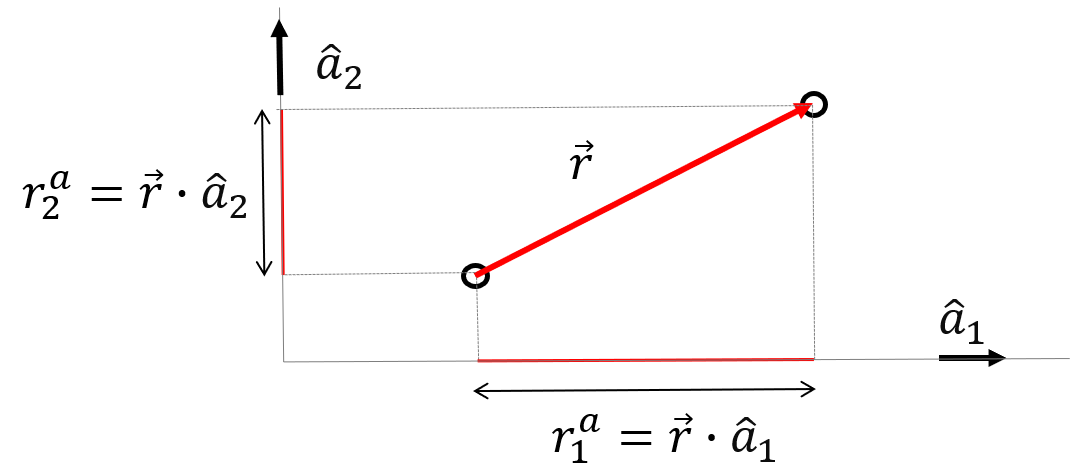
\includegraphics[width=0.50\textwidth]{vecpospro2.png}
				\label{fig:vecpospro2}}
				\hspace{+20pt}
				\subfloat[Décomposition selon les directions de la base]{
				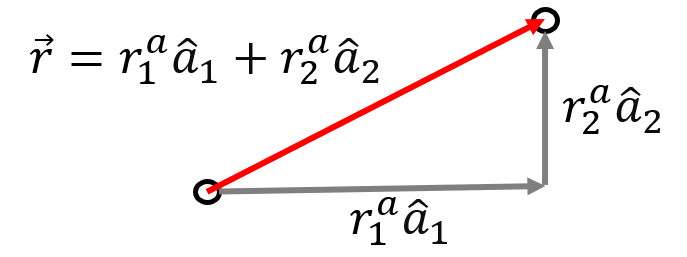
\includegraphics[width=0.40\textwidth]{vecpospro3.png}
				\label{fig:vecpospro3}}
				%\vspace{+30pt}
        \caption{Relations entre le vecteur géométrique de position et les composantes du vecteur-colonne}
				\label{fig:vecpospro23}
\end{figure}
%%%%%%%%%%%%%%%%%%%%%%%%%%%%%%%%%%%%%%%%%%%%%%%%%%%%%%%%%%%%%%%%%


%%%%%%%%%%%%%%%%%%%%%%%%%%%%%%%%%%%%%%%%%%%%%%%%%%%
\subsection{Transfert d'une équation vectorielle vers une équation matricielle} 
%
Lorsque les composantes de plusieurs vecteurs-géométrique de position sont exprimées avec la même base, il est possible de faire des opérations directement avec les vecteur-colonnes de composantes. Cela permet de traiter simultanément les calculs de plusieurs axes, et aussi de faire des calculs numériques efficaces en utilisant les outils de l'algèbre linéaire. Par exemple, les additions et soustractions de vecteurs géométriques peuvent être calculées directement en termes des vecteur-colonnes dans une base:
%%%%%%%%%%%%%%%%%%%%%%%%%%%%%%%%%%%
\begin{equation}
\vec{r}_{A/C}   = \vec{r}_{A/B} + \vec{r}_{B/C}   \quad \Rightarrow \quad
\col{r}_{A/C}^a = \col{r}_{A/B}^a + \col{r}_{B/C}^a
\end{equation} 
%%%%%%%%%%%%%%%%%%%%%%%%%%%%%%%%%%%
Ce transfert d'une seule équation vectorielle à une équation matricielle (équivalent à un système de trois équations scalaires) correspond à une projection de l'équation vectorielle sur chacun des axes de la base:
%%%%%%%%%%%%%%%%%%%%%%%%%%%%%%%%%%%
\begin{equation}
\vec{r}_{A/C}   = \vec{r}_{A/B} + \vec{r}_{B/C}  
\quad \Rightarrow \quad
\left[ \begin{array}{c} (\vec{r}_{A/C}   = \vec{r}_{A/B} + \vec{r}_{B/C}   ) \bullet \hat{a}_1 \\ (\vec{r}_{A/C}   = \vec{r}_{A/B} + \vec{r}_{B/C}   ) \bullet \hat{a}_2 \\ (\vec{r}_{A/C}   = \vec{r}_{A/B} + \vec{r}_{B/C}  ) \bullet \hat{a}_3  \end{array} \right] 
\quad \Rightarrow \quad
\col{r}_{A/C}^a = \col{r}_{A/B}^a + \col{r}_{B/C}^a
\end{equation} 
%%%%%%%%%%%%%%%%%%%%%%%%%%%%%%%%%%%

Les équations vectorielles avec des vecteurs de position peuvent donc être substituées par des équations matricielles équivalentes avec les vecteur-colonnes,\textbf{ à condition que tous les vecteur-colonnes soient exprimés dans une base commune}. 
  

% Voici quelques exemples de substitution d'équation de vecteurs de position vers des équations matricielles:
% %%%%%%%%%%%%%%%%%%%%%%%%%%%%%%%%%%%
% \begin{align}
% \vec{r}_{B/C}   = \vec{r}_{B/A} - \vec{r}_{C/A}   
% \quad &\Rightarrow \quad  \col{r}_{B/C}^a   = \col{r}_{B/A}^a - \col{r}_{C/A}^a 
% \\
% \vec{r}_{B/C}   = \vec{r}_{B/A} - \vec{r}_{C/A} \quad &\Rightarrow \quad \col{r}_{B/C}^b   = \col{r}_{B/A}^b - \col{r}_{C/A}^b 
% \\
% 2  \vec{r}_{D/A} = 3 \vec{r}_{B/A} + \vec{r}_{C/A} \quad &\Rightarrow \quad  2  \col{r}_{D/A}^a = 3 \col{r}_{B/A}^a + \col{r}_{C/A}^a
% \end{align} 
% %%%%%%%%%%%%%%%%%%%%%%%%%%%%%%%%%%%

%%%%%%%%%%%%%%%%%%%%%%%%%%%%%%%%%%%%%%%%%%%%%%%%%%%%%%%%%%%%%%%%%
\note{Programmation de calculs de cinématique:}{ Lors de l'écriture d'un programme informatique pour effectuer des calculs de cinématique, les calculs numériques doivent être fait en termes de composantes. En effet, les ordinateurs sont adaptés à manipuler des chiffres, des vecteur-colonnes de chiffres, des matrices de chiffres, etc. Toutefois, un ordinateur ne peut manipuler directement des éléments conceptuels comme les vecteurs unitaires.}
%%%%%%%%%%%%%%%%%%%%%%%%%%%%%%%%%%%%%%%%%%%%%%%%%%%%%%%%%%%%%%%%%

% %%%%%%%%%%%%%%%%%%%%%%%%%%%%%%%%%%%%%%%%%%%%%%%%%%%
% \subsection{Opérations avec les vecteur-colonnes} 
% %
% Les opérations vectorielles ont des équivalents en termes d'opérations matricielle avec les vecteur-colonnes qui sont très utiles pour les calculs numériques. Cette section introduit les opérations principales utiles pour la cinématique.

% \subsubsection{Produit scalaire}
% Un produit scalaire peut être calculé directement par une opération matricielle avec les vecteur-colonnes appelée produit intérieur (\textit{inner product}):
% %%%%%%%%%%%%%%%%%%%%%%%%%%%%%%%%%%%
% \begin{equation}
% \vec{u} \bullet \vec{v} = \col{u}^T \col{v} = \left[ \begin{array}{c c c} u_1 & u_2 & u_3  \end{array} \right]  \left[ \begin{array}{c} v_1 \\ v_2 \\ v_3  \end{array} \right]
% = u_1 v_1 + u_2 v_2 + u_3 v_3
% \end{equation} 
% %%%%%%%%%%%%%%%%%%%%%%%%%%%%%%%%%%%
% si $\col{u}$ et $\col{v}$ sont les composantes exprimées dans une base vectorielle commune, par exemple:
% %%%%%%%%%%%%%%%%%%%%%%%%%%%%%%%%%%%
% \begin{align}
% \vec{u} \bullet \vec{v} &= (\col{u}^a)^T \col{v}^a = (\col{u}^b)^T \col{v}^b
% \end{align} 
% %%%%%%%%%%%%%%%%%%%%%%%%%%%%%%%%%%%
% mais attention car: 
% %%%%%%%%%%%%%%%%%%%%%%%%%%%%%%%%%%%
% \begin{align}
% \vec{u} \bullet \vec{v} &\ne (\col{u}^a)^T \col{v}^b \\
% \vec{u} \bullet \vec{v} &\ne (\col{u}^b)^T \col{v}^a 
% \end{align} 
% %%%%%%%%%%%%%%%%%%%%%%%%%%%%%%%%%%%
% Il est à noter que l'ordre de multiplication ne change pas le résultat pour le produit scalaire:
% %%%%%%%%%%%%%%%%%%%%%%%%%%%%%%%%%%%
% \begin{equation}
% \vec{u} \bullet \vec{v} = \vec{v} \bullet \vec{u} = \col{u}^T \col{v} = \col{v}^T \col{u} 
% \end{equation} 
% %%%%%%%%%%%%%%%%%%%%%%%%%%%%%%%%%%%

\subsection{Calcul de longueurs, projections et angles avec les composantes}
Lorsqu'on connaît les composantes d'un vecteur position $\vec{r}$, le produit intérieur peut être utilisé pour calculer sa longueur:
%%%%%%%%%%%%%%%%%%%%%%%%%%%%%%%%%%%
\begin{align}
\|\vec{r}\|^2 &= \vec{r} \bullet \vec{r} = \col{r}^T \col{r} = r_1^2 + r_2^2 + r_3^2  \\
\|\vec{r}\|  &= \sqrt{ \col{r}^T \col{r} }
\end{align} 
%%%%%%%%%%%%%%%%%%%%%%%%%%%%%%%%%%%
pour calculer une distance projetée selon un axe décrit par un vecteur unitaire $\hat{n}$:
%%%%%%%%%%%%%%%%%%%%%%%%%%%%%%%%%%%
\begin{align}
d_n &= \vec{r} \bullet \hat{n} = \col{r}^T \col{n} = 
\left[ \begin{array}{c c c} r_1 &  r_2 &  r_3  \end{array} \right]
\left[ \begin{array}{c}     n_1 \\ n_2 \\ n_3  \end{array} \right]
= r_1 n_1 + r_2 n_2 + r_3 n_3
\end{align} 
%%%%%%%%%%%%%%%%%%%%%%%%%%%%%%%%%%%
pour calculer un angle entre deux vecteurs unitaires $\hat{x}$ et $\hat{y}$:
%%%%%%%%%%%%%%%%%%%%%%%%%%%%%%%%%%%
\begin{align}
\cos \angle (\hat{x},\hat{y}) &= \hat{x} \bullet \hat{y} = \col{x}^T \col{y} \\
\angle (\hat{x},\hat{y}) &= \arccos{ ( \col{x}^T \col{y} ) } 
\end{align} 
%%%%%%%%%%%%%%%%%%%%%%%%%%%%%%%%%%%
et pour calculer entre deux vecteurs position $\vec{r}_A$ et $\vec{r}_B$:
%%%%%%%%%%%%%%%%%%%%%%%%%%%%%%%%%%%
\begin{align}
\vec{r}_A \bullet \vec{r}_B = \|\vec{r}_A\|  \|\vec{r}_B\|  \cos \angle (\vec{r}_A,\vec{r}_B) &= \col{r}_A^T \col{r}_B \\
\angle (\vec{r}_A,\vec{r}_B) &= \arccos{ \left( \frac{\col{r}_A^T \col{r}_B }{ \sqrt{ \col{r}_A^T \col{r}_A} \, \sqrt{ \col{r}_B^T \col{r}_B}} \right) }
\end{align} 
%%%%%%%%%%%%%%%%%%%%%%%%%%%%%%%%%%%
%
Il est à noter que dans ces équations les vecteur-colonnes de composantes doivent tous être dans la même base. Les résultats sont des scalaires qui ne dépendent pas de la base utilisée. 

\video{Opérations vectorielles avec les composantes de vecteurs}{https://youtu.be/7brvShmayAk}

% %%%%%%%%%%%%%%%%%%%%%%%%%%%%%%%%%%%
% \subsubsection{Produit vectoriel}
% %
% Un produit vectoriel (\textit{cross product}) peut être calculé directement par une opération matricielle définie avec les vecteur-colonnes:
% %%%%%%%%%%%%%%%%%%%%%%%%%%%%%%%%%%%
% \begin{equation}
% \vec{u} = \vec{v} \times \vec{w} \quad \Rightarrow \quad  \col{u} = \col{v}^{\times}\col{w} \quad \Rightarrow \quad 
%  \left[ \begin{array}{c} u_1 \\ u_2 \\ u_3  \end{array} \right] = 
% \left[ \begin{array}{c c c}
% 	0 & -v_3 & v_2  \\ v_3 & 0 & -v_1 \\ -v_2 & v_1 & 0
% \end{array}  \right]
%  \left[ \begin{array}{c} w_1 \\ w_2 \\ w_3  \end{array} \right]
% \end{equation} 
% %%%%%%%%%%%%%%%%%%%%%%%%%%%%%%%%%%%
% L'ordre de multiplication est important pour le produit vectoriel, il change la direction du vecteur résultant:
% %%%%%%%%%%%%%%%%%%%%%%%%%%%%%%%%%%%
% \begin{equation}
% \vec{u} = \vec{v} \times \vec{w} =  -\vec{w} \times \vec{v} \quad \Rightarrow \quad  \col{u} = \col{v}^{\times}\col{w} = - \col{w}^{\times}\col{v}
% \end{equation} 
% %%%%%%%%%%%%%%%%%%%%%%%%%%%%%%%%%%%

% \paragraph{Vecteurs unitaires d'une base vectorielle:}
% Il est possible de calculer les composantes d'un vecteur unitaire qui complète une base vectorielle avec une opération de produit vectorielle, connaissant les composantes de deux vecteurs unitaires orthogonaux: 
% %%%%%%%%%%%%%%%%%%%%%%%%%%%%%%%%%%%
% \begin{equation}
% \hat{b}_3 = \hat{b}_1 \times \hat{b}_2  \quad \Rightarrow \quad   \col{b}_3 = \col{b}_1^{\times}\col{b}_2
% \end{equation} 
% %%%%%%%%%%%%%%%%%%%%%%%%%%%%%%%%%%%

% \paragraph{Note:}
% Pour alléger la présentation, les exposants qui spécifient les bases vectorielles associées aux vecteur-colonnes sont parfois omis dans les équations, on considère alors que tous les vecteur-colonnes impliqués dans l'équation sont exprimés dans une base vectorielle commune.


% %%%%%%%%%%%%%%%%%%%%%%%%%%%%%%%%%%%
% \subsubsection{Changement de base}
% %
% Les composantes d'un vecteur géométrique $\vec{v}$ dans une base $a$ peuvent être directement reliées aux composantes du même vecteur géométrique $\vec{v}$ dans une autre base $b$, par une équation matricielle qui implique les vecteur-colonnes et une matrice 3$\times$3 appelée une \textit{matrice de rotation}. On va noter une matrice $^bR^a$ lorsqu'une multiplication par la gauche de cette matrice avec un vecteur colonne $\col{v}^a$ donne le vecteur-colonne $\col{v}^b$:
% %%%%%%%%%%%%%%%%
% \begin{align}
% \col{v}^b &= {}^bR^a \col{v}^a  \quad \Rightarrow \quad
%  \left[ \begin{array}{c} v_1^b \\ v_2^b \\ v_3^b  \end{array} \right]
% =
% \left[ \begin{array}{c c c}
% 	{}^bR^a_{11} & {}^bR^a_{12} & {}^bR^a_{13} \\ 
% 	{}^bR^a_{21} & {}^bR^a_{22} & {}^bR^a_{23} \\
% 	{}^bR^a_{31} & {}^bR^a_{32} & {}^bR^a_{33}
% \end{array}  \right]
%  \left[ \begin{array}{c} v_1^a \\ v_2^a \\ v_3^a  \end{array} \right]
% \label{eq:basechange1}
% \end{align} 
% %%%%%%%%%%%%%%%%%
% Les propriétés et le calcul des matrices de rotation seront traités en détails à la section \ref{sec:changematrice}.



%%%%%%%%%%%%%%%%%%%%%%%%%%%%%%%%%%%%%%%%%%%%%%%%%%%%
%\subsection{Calculs appliqués dans un contexte de cinématique} 
%%
%\paragraph{Normes, projections et calcul d'angles:}
%Lorsque qu'on connait les composantes de vecteurs dans une base commune, le produit intérieur peut être utilisé pour calculer la longueur d'un vecteur position:
%%%%%%%%%%%%%%%%%%%%%%%%%%%%%%%%%%%%
%\begin{align}
%\|\vec{r}\|^2 &= \vec{r} \bullet \vec{r} = \col{r}^T \col{r} = r_1^2 + r_2^2 + r_3^2
%\end{align} 
%%%%%%%%%%%%%%%%%%%%%%%%%%%%%%%%%%%%
%pour calculer une distance projeté selon un axe décrit par un vecteur unitaire $\hat{n}$:
%%%%%%%%%%%%%%%%%%%%%%%%%%%%%%%%%%%%
%\begin{align}
%d_n &= \vec{r} \bullet \hat{n} = \col{r}^T \col{n} = r_1 n_1 + r_2 n_2 + r_3 n_3
%\end{align} 
%%%%%%%%%%%%%%%%%%%%%%%%%%%%%%%%%%%%
%et pour calculer un angle entre deux vecteurs unitaires $\hat{x}$ et $\hat{y}$:
%%%%%%%%%%%%%%%%%%%%%%%%%%%%%%%%%%%%
%\begin{align}
%\cos \angle (\hat{x},\hat{y}) = \hat{x} \bullet \hat{y} = \col{x}^T \col{y} = x_1 y_1 + x_2 y_2 + x_3 y_3
%\end{align} 
%%%%%%%%%%%%%%%%%%%%%%%%%%%%%%%%%%%%
%
%\paragraph{Vecteurs unitaires:}
%Il est possible de calculer les composantes d'un vecteur unitaire qui complète une base vectorielle avec une opération de produit vectorielle, connaissant les composantes de deux vecteurs unitaires orthogonaux: 
%%%%%%%%%%%%%%%%%%%%%%%%%%%%%%%%%%%%
%\begin{equation}
%\hat{b}_3 = \hat{b}_1 \times \hat{b}_2  \quad \Rightarrow \quad   \col{b}_3 = \col{b}_1^{\times}\col{b}_2
%\end{equation} 
%%%%%%%%%%%%%%%%%%%%%%%%%%%%%%%%%%%%


% %%%%%%%%%%%%%%%%%%%%%%%%%%%%%%%%%%%%%%%%%%%%%%%%%%%
% \subsection{Invariants} 
% %
% Le vecteur géométrique $\vec{r}$ est une quantité constante peu importe la base vectorielle utilisée: 
% %%%%%%%%%%%%%%%
% \begin{equation}
% \vec{r} = \sum_{i} r_i^a \hat{a}_i = \sum_{i} r_i^b \hat{b}_i = \sum_{i} r_i^c \hat{c}_i
% \end{equation}
% %%%%%%%%%%%%%%%
% mais le vecteur-colonne dépend de la base vectorielle. Les vecteur-colonnes sont en générale différents sauf dans le cas particulier de bases vectorielles coïncidentes:
% %%%%%%%%%%%%%%%%%%%%%%%%%%%%%%%%%%%
% \begin{equation}
% \col{r}^{a} \ne \col{r}^{b} \quad\quad \text{sauf dans le cas particulier:} \quad \hat{a}_1 = \hat{b}_1 \;,\; \hat{a}_2 = \hat{b}_2  \;\text{et}\; \hat{a}_3 = \hat{b}_3 
% \end{equation} 
% %%%%%%%%%%%%%%%%%%%%%%%%%%%%%%%%%%%
% La longueur du vecteur géométrique étant une constante peut importe la base vectorielle utilisée, il est possible d'établir la relation suivante entre les vecteur-colonnes utilisant différentes bases:
% %%%%%%%%%%%%%%%
% \begin{equation}
% \|\vec{r}\|^2 = \vec{r} \bullet \vec{r} = (\col{r}^{a})^T \col{r}^{a} = (\col{r}^{b})^T \col{r}^{b} = (\col{r}^{c})^T \col{r}^{c}
% \end{equation}
% %%%%%%%%%%%%%%%
% La norme des vecteur-colonnes est donc invariante par rapport au choix de la base. 








%%%%%%%%%%%%%%%%%%%%%%%%%%%%%%%%%%%%%%%%%%%%%%%%%%%%%%%%%%%%%%%%%%%%%%\new
\newpage
\section{Les matrices de rotations}
\label{sec:changematrice}

Une matrice de rotation notée $^aR^b$, est une matrice (3$\times$3 en 3D) qui permet de calculer directement les composants d'un vecteur position dans une base $a$ avec les composants connus dans une base $b$, i.e. effectuer un \textbf{changement de base}, par une multiplication de la forme:
%%%%%%%%%%%%%%%%
\begin{align}
\col{r}^a &= {}^aR^b \col{r}^b
\label{eq:basechange}
\end{align} 
%%%%%%%%%%%%%%%%%
La matrice de rotation est un raccourci pour projeter un vecteur position sur trois nouveaux axes en une seule opération matricielle, plutôt que d'effectuer trois opérations de projection indépendantes. Cette matrice représente l'orientation relative de deux bases vectorielles et  \textbf{l'opération de multiplication d'un vecteur-colonne $\col{r}^a$ par la matrice de rotation $^bR^a$ correspond à la projection du vecteur géométrique associé $\vec{r}$ sur la base vectorielle $b$.}

%%%%%%%%%%%%%%%%%%%%%%%%%%%%%%%%%%%%%%%%%%%%%%%%%%%%%%%%%%%%%%%%%
\note{Deux rôles pour la cinématique:}{ Une matrice de rotation a deux fonctions majeures dans un contexte de cinématique: \textbf{1)} effectuer des opérations de changement de base et \textbf{2)} représenter une orientation relative. Cette section présente le rôle des matrices de rotation pour les opérations de changement de base, les matrices de rotation seront discutées à nouveau dans le contexte de la représentation de l'orientation d'un corps rigide à la section \ref{sec:corps}.}
%%%%%%%%%%%%%%%%%%%%%%%%%%%%%%%%%%%%%%%%%%%%%%%%%%%%%%%%%%%%%%%%%

\video{Les matrices de rotation et les changements de base}{https://youtu.be/hVmcRYD1KFQ}

%%%%%%%%%%%%%%%%%%%%%%%%%%%%%%%%%%%%%%%%%%%%%%%%%%%%%%%%%%%%%
\subsection{Définitions}

Une matrice de rotation est définie par les produits scalaires des vecteurs unitaires qui forment deux bases vectorielles:
%%%%%%%%%%%%%%%%%%%%%%%%%%%%%%%%%%%
\begin{align}
{}^aR^b &= 
\left[ \begin{array}{c c c} 
\hat{a}_1 \bullet \hat{b}_1  &  \hat{a}_1 \bullet \hat{b}_2  &  \hat{a}_1 \bullet \hat{b}_3 \\
\hat{a}_2 \bullet \hat{b}_1  &  \hat{a}_2 \bullet \hat{b}_2  &  \hat{a}_2 \bullet \hat{b}_3 \\
\hat{a}_3 \bullet \hat{b}_1  &  \hat{a}_3 \bullet \hat{b}_2  &  \hat{a}_3 \bullet \hat{b}_3 
\end{array} \right] 
= 
\left[ \begin{array}{c c c} 
\cos \angle (\hat{a}_1 , \hat{b}_1)  &  \cos \angle (\hat{a}_1 , \hat{b}_2)  &  \cos \angle (\hat{a}_1 , \hat{b}_3) \\
\cos \angle (\hat{a}_2 , \hat{b}_1)  &  \cos \angle (\hat{a}_2 , \hat{b}_2)  &  \cos \angle (\hat{a}_2 , \hat{b}_3) \\
\cos \angle (\hat{a}_3 , \hat{b}_1)  &  \cos \angle (\hat{a}_3 , \hat{b}_2)  &  \cos \angle (\hat{a}_3 , \hat{b}_3) 
\end{array} \right]
\label{eq:cosinusdirecteurs}
\end{align} 
%%%%%%%%%%%%%%%%%%%%%%%%%%%%%%%%%%%
Les produits scalaires correspondent aussi aux cosinus des angles entre les vecteurs unitaires, c'est pourquoi la matrice de rotation est aussi parfois appelée la \textbf{matrice des cosinus directeurs}. Par inspection de l'équation \eqref{eq:cosinusdirecteurs}, on remarque que les colonnes de la matrice ${}^aR^b$ correspondent aux vecteur-colonnes des composantes des vecteurs unitaires $\hat{b}_i$ exprimées dans la base $a$ et que les rangés de la matrice ${}^aR^b$ correspondent à la transposée des vecteur-colonnes des composantes des vecteurs unitaires $\hat{a}_i$ exprimées dans la base $b$. Cela permet donc des définitions équivalentes plus compactes:
%%%%%%%%%%%%%%%%%%%%%%%%%%%%%%%%%%%
\begin{align}
{}^aR^b &= 
%\left[ \begin{array}{c c c} 
%\col{b}_1^a &  \col{b}_2^a & \col{b}_3^a
%\end{array} \right] 
%=
%\left[ \begin{array}{c} 
%(\col{a}_1^b)^T \\
%(\col{a}_2^b)^T \\
%(\col{a}_3^b)^T
%\end{array} \right] = 
\left[ \begin{array}{c c c} 
	\left[ \begin{array}{c} \\ \col{b}_1^a \\  \\ \end{array}  \right] & \left[ \begin{array}{c} \\ \col{b}_2^a \\  \\ \end{array}  \right] & \left[ \begin{array}{c} \\ \col{b}_3^a \\  \\ \end{array}  \right]
\end{array} \right]
=
\left[ \begin{array}{c} 
\left[ \begin{array}{c c c} & (\col{a}_1^b)^T & \end{array} \right] \\[\medskipamount]
\left[ \begin{array}{c c c} & (\col{a}_2^b)^T & \end{array} \right] \\[\medskipamount]
\left[ \begin{array}{c c c} & (\col{a}_3^b)^T & \end{array} \right] 
\end{array} \right] 
\label{eq:matricerotcol}
\end{align} 
%%%%%%%%%%%%%%%%%%%%%%%%%%%%%%%%%%%
Finalement, la matrice de rotation peut aussi être définie en termes de composantes et d'indices par:
%%%%%%%%%%%%%%%%%%%%%%%%%%%%%%%%%%%
\begin{align}
{}^aR^b_{ij} &= \hat{a}_i \bullet \hat{b}_j
\end{align} 
%%%%%%%%%%%%%%%%%%%%%%%%%%%%%%%%%%%
une équation qui est simple à se rappeler et permet d'éviter de mélanger l'ordre de rotation ${}^aR^b$ vs. ${}^bR^a$ avec la notation utilisée dans ces notes.






%%%%%%%%%%%%%%%%%%%%%%%%%%%%%%%%%%%%%%%
%\subsection{Démonstration de l'origine de la matrice de rotation}
%Cette section démontre l'équation \eqref{eq:basechange} basé sur les définitions des vecteur-colonnes de composants. 
\begin{proof}
Si les composantes d'un vecteur $\vec{r}$ sont connus dans une base $a$:
%%%%%%%%%%%%%%%%%%%%%%%%%%%%%%%%%%%
\begin{align}
\col{r}^a &= \left[ \begin{array}{c} r_1^a \\ r_2^a \\ r_3^a  \end{array} \right]
\end{align} 
%%%%%%%%%%%%%%%%%%%%%%%%%%%%%%%%%%%
le vecteur géométrique associé est donné par:
%%%%%%%%%%%%%%%%%%%%%%%%%%%%%%%%%%%
\begin{align}
\vec{r} &= r_1^a \hat{a}_1 + r_2^a \hat{a}_2 + r_3^a \hat{a}_3
\label{eq:pvec}
\end{align} 
%%%%%%%%%%%%%%%%%%%%%%%%%%%%%%%%%%%
Les composantes dans une base $b$ peuvent être calculées par des produits scalaires suivants:
%%%%%%%%%%%%%%%%%%%%%%%%%%%%%%%%%%%
\begin{align}
r_1^b &= \vec{r} \bullet \hat{b}_1 \\
r_2^b &= \vec{r} \bullet \hat{b}_2 \\
r_3^b &= \vec{r} \bullet \hat{b}_3
\end{align} 
%%%%%%%%%%%%%%%%%%%%%%%%%%%%%%%%%%%
Si on substitue $\vec{r}$ par l'équation \eqref{eq:pvec}:
%%%%%%%%%%%%%%%%%%%%%%%%%%%%%%%%%%%
\begin{align}
r_1^b &= (r_1^a \hat{a}_1 + r_2^a \hat{a}_2 + r_3^a \hat{a}_3) \bullet \hat{b}_1 \\
r_2^b &= (r_1^a \hat{a}_1 + r_2^a \hat{a}_2 + r_3^a \hat{a}_3) \bullet \hat{b}_2 \\
r_3^b &= (r_1^a \hat{a}_1 + r_2^a \hat{a}_2 + r_3^a \hat{a}_3) \bullet \hat{b}_3
\end{align} 
%%%%%%%%%%%%%%%%%%%%%%%%%%%%%%%%%%%
et on réarrange les termes:
%%%%%%%%%%%%%%%%%%%%%%%%%%%%%%%%%%%
\begin{align}
r_1^b &= (\hat{a}_1 \bullet \hat{b}_1 ) r_1^a + (\hat{a}_2 \bullet \hat{b}_1 ) r_2^a + (\hat{a}_3 \bullet \hat{b}_1 ) r_3^a \\
r_2^b &= (\hat{a}_1 \bullet \hat{b}_2 ) r_1^a + (\hat{a}_2 \bullet \hat{b}_2 ) r_2^a + (\hat{a}_3 \bullet \hat{b}_2 ) r_3^a \\
r_3^b &= (\hat{a}_1 \bullet \hat{b}_3 ) r_1^a + (\hat{a}_2 \bullet \hat{b}_3 ) r_2^a + (\hat{a}_3 \bullet \hat{b}_3 ) r_3^a 
\end{align} 
%%%%%%%%%%%%%%%%%%%%%%%%%%%%%%%%%%%
On obtient trois équations qui peuvent être regroupées sous forme matricielle:
%%%%%%%%%%%%%%%%%%%%%%%%%%%%%%%%%%%
\begin{align}
\underbrace{ \left[ \begin{array}{c} r_1^b \\ r_2^b \\ r_3^b  \end{array} \right] }_{\col{r}^b}
=
\underbrace{ \left[ \begin{array}{c c c} 
\hat{a}_1 \bullet \hat{b}_1 & \hat{a}_2 \bullet \hat{b}_1 & \hat{a}_3 \bullet \hat{b}_1 \\
\hat{a}_1 \bullet \hat{b}_2 & \hat{a}_2 \bullet \hat{b}_2 & \hat{a}_3 \bullet \hat{b}_2 \\
\hat{a}_1 \bullet \hat{b}_3 & \hat{a}_2 \bullet \hat{b}_3 & \hat{a}_3 \bullet \hat{b}_3 
\end{array} \right] }_{^bR^a}
\underbrace{ \left[ \begin{array}{c} r_1^a \\ r_2^a \\ r_3^a  \end{array} \right] }_{\col{r}^a}
\label{eq:Rdot}
\end{align} 
%%%%%%%%%%%%%%%%%%%%%%%%%%%%%%%%%%%

La matrice de rotation $^bR^a$ consiste donc à des produits scalaires entre les vecteurs unitaires des bases vectorielles $a$ et $b$ comme définit à l'équation \eqref{eq:cosinusdirecteurs}.
\end{proof}





%%%%%%%%%%%%%%%%%%%%%%%%%%%%%%%%%%%%%%%
\begin{example}[Matrice de rotation dans le plan calculée par trigonométrie]

La figure \ref{fig:basechange2d} montre un exemple d'un vecteur $\vec{r}$ en 2 dimensions exprimé dans deux base vectorielles $b$ et $a$. Comme illustré à la figure \ref{fig:r_trigo}, avec une construction de triangles il est possible de déterminer par trigonométrie les relations entre les composantes dans les deux bases, et donc la matrice de rotation ${}^aR^b$. L'approche par trigonométrie est toutefois limitée pour les rotations en 3D, une approche vectorielle plus simple et plus universelle pour calculer des matrices de rotation est présentée à la section \ref{sec:calmat}.
%%%%%%%%%%%%%
\begin{figure}[H]
	\centering
		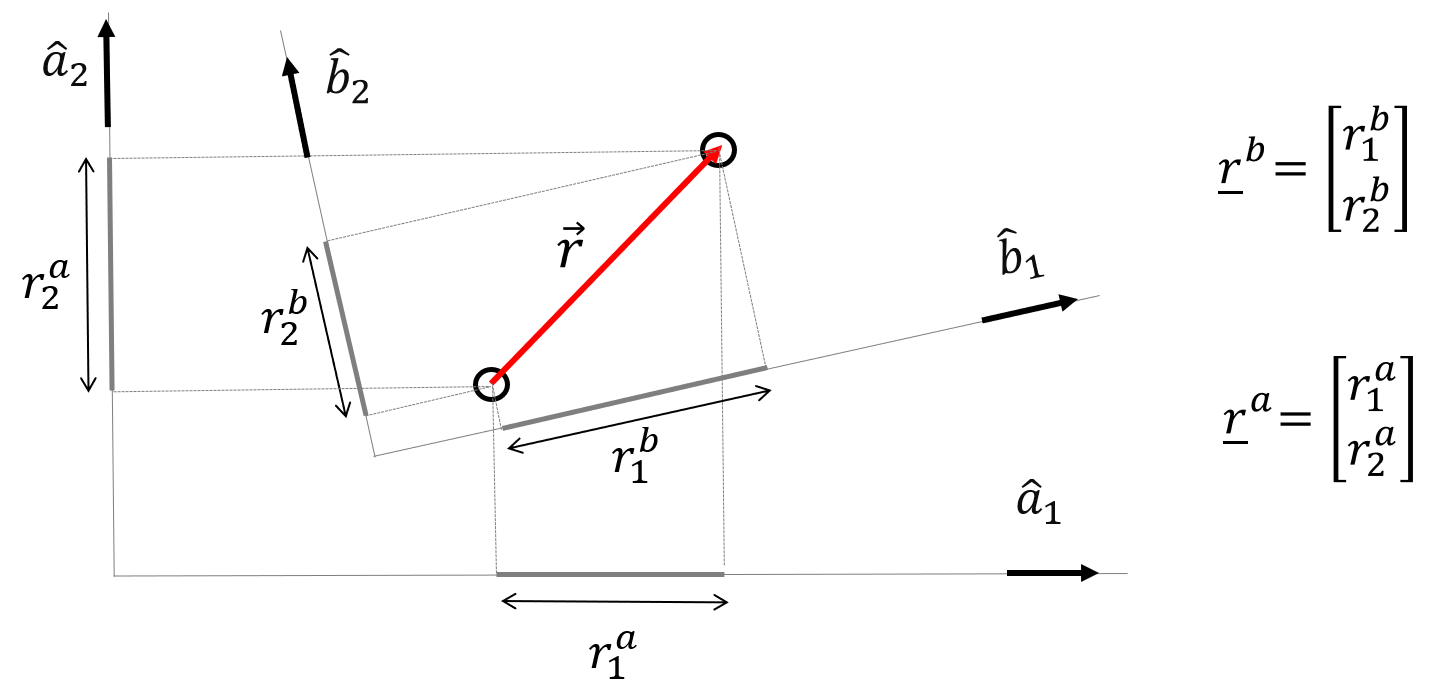
\includegraphics[width=0.65\textwidth]{basechange.png}
	\caption{Vecteur position exprimé dans deux bases vectorielles}
	\label{fig:basechange2d}
\end{figure}
%%%%%%%%%%%%%%
%%%%%%%%%%%%%
\begin{figure}[H]
	\centering
		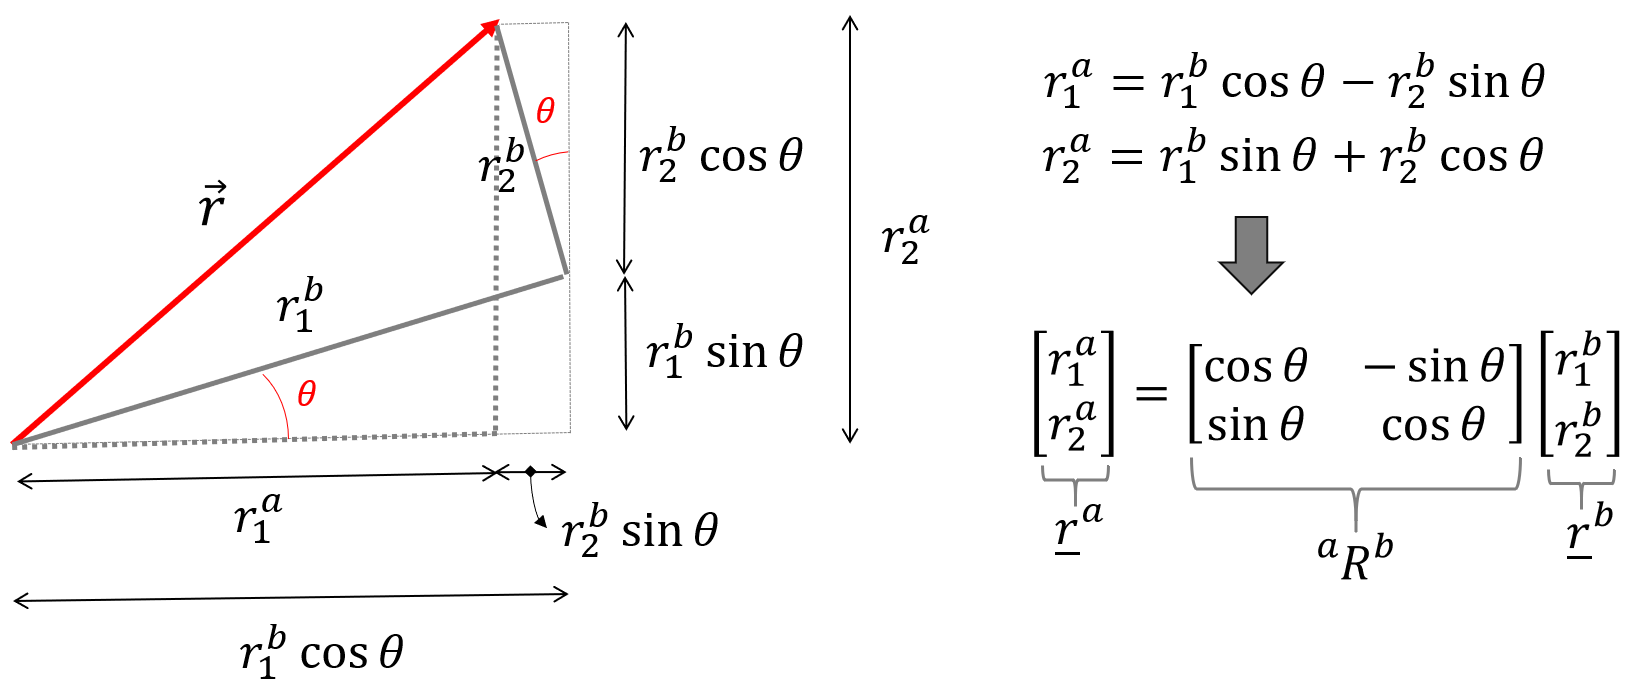
\includegraphics[width=0.65\textwidth]{r_trigo.png}
	\caption{Calcul par trigonométrie de la matrice de rotation 2x2 ${}^aR^b$ pour le changement de base illustré à la figure \ref{fig:basechange2d}}
	\label{fig:r_trigo}
\end{figure}
%%%%%%%%%%%%%%

\end{example} 



%%%%%%%%%%%%%%%%%%%%%%%%%%%%%%%%%%%
\subsection{Méthode de calcul des matrices de rotation basé sur les colonnes}
\label{sec:calmat}

La définition des matrices de rotation basée sur les vecteurs unitaires de eq.\eqref{eq:matricerotcol} est particulièrement utile pour calculer une matrice de rotation. Une astuce pour ne pas mélanger l'ordre de rotation ($^bR^a$ vs. $^aR^b$) est d'avoir en tête que la multiplication matricielle c'est une combinaison linéaire de vecteur-colonnes:
%%%%%%%%%%%%%%%%%%%%%%%%%%%
\begin{align}
\col{r}^a &= 
\underbrace{ \left[ \begin{array}{c c c} 
	\left[ \begin{array}{c} \\ \col{b}_1^a \\  \\ \end{array}  \right] & \left[ \begin{array}{c} \\ \col{b}_2^a \\  \\ \end{array}  \right] & \left[ \begin{array}{c} \\ \col{b}_3^a \\  \\ \end{array}  \right]
\end{array} \right] }_{^aR^b}
\underbrace{ \left[ \begin{array}{c} r_1^b \\ r_2^b \\ r_3^b  \end{array} \right] }_{\col{r}^b}
= 
\left[ \begin{array}{c} \\ \col{b}_1^a \\  \\ \end{array}  \right] \, r_1^b + \left[ \begin{array}{c} \\ \col{b}_2^a \\  \\ \end{array}  \right]\, r_2^b + \left[ \begin{array}{c} \\ \col{b}_3^a \\  \\ \end{array}  \right] \, r_3^b 
\end{align}
%%%%%%%%%%%%%%%%%%%%%%%%%%%%%%%%
% TODO figure combinaisons de vecteur colonnes?
%%%%%%%%%%%%%%%%%%%%%%%%%%%%%%%%%%%
et donc que si on cherche la matrice de rotation ${}^aR^b$ pour calculer le passage de la base $b$ vers la base $a$, il faut trouver les directions spatiales $\hat{b}_1$, $\hat{b}_2$ et $\hat{b}_3$ qui seront combinées linéairement selon les coeficients $r_1^b$, $r_2^b$, $r_3^b$. 

%Une méthode rapide et universelle pour calculer une matrice de rotation est de \textbf{1)} construire par inspection les vecteur unitaires $\hat{b}_i$ de la base vectorielle initiale, comme une combinaison de vecteur unitaires $\hat{a}_i$ de la base cible, \textbf{2)} convertir les équations en vecteur-colonnes $\col{b}_i^a$, et \textbf{3)} assembler la matrice avec la définition de l'équation \eqref{eq:matricerotcol}:
%%%%%%%%%%%%%%%%%%%%%%%%%%%%%%%%%%%%
%\begin{align}
%\hat{b}_1 &= a \, \hat{a}_1 + b \, \hat{a}_2 + c \, \hat{a}_3  \quad\quad  \hat{b}_2 = d \, \hat{a}_1 + e \, \hat{a}_2 + f \, \hat{a}_3   \quad\quad  \hat{b}_3 = g \, \hat{a}_1 + h \, \hat{a}_2 + i \, \hat{a}_3  \\
%\col{b}_1^a  &= \left[ \begin{array}{c} a \\ b \\ c  \end{array} \right] \quad\quad\quad\quad\quad\quad\;  
%\col{b}_2^a  = \left[ \begin{array}{c} d \\ e \\ f  \end{array} \right]  \quad\quad\quad\quad\quad\quad\; 
%\col{b}_3^a  = \left[ \begin{array}{c} g \\ h \\ i  \end{array} \right]  \\
%{}^aR^b = 
%\left[ \begin{array}{c c c} 
%\col{b}_1^a &  \col{b}_2^a & \col{b}_3^a
%\end{array} \right] 
%=
%\left[ \begin{array}{c c c} 
%a & d & g \\ 
%b & e & h \\ 
%c & f & i 
%\end{array} \right]
%\end{align} 
%%%%%%%%%%%%%%%%%%%%%%%%%%%%%%%%%%%%

Une méthode rapide et universelle pour calculer une matrice de rotation est de construire par inspection les vecteur unitaires $\hat{b}_i$ de la base vectorielle initiale, comme une combinaison de vecteurs unitaires $\hat{a}_i$ de la base cible:
%%%%%%%%%%%%%%%%%%%%%%%%%%%%%%%%%%%
\begin{align}
\hat{b}_1 &= a \, \hat{a}_1 + b \, \hat{a}_2 + c \, \hat{a}_3  \quad\quad  \hat{b}_2 = d \, \hat{a}_1 + e \, \hat{a}_2 + f \, \hat{a}_3   \quad\quad  \hat{b}_3 = g \, \hat{a}_1 + h \, \hat{a}_2 + i \, \hat{a}_3 
\end{align} 
%%%%%%%%%%%%%%%%%%%%%%%%%%%%%%%%%%%
pour ensuite convertir les équations en vecteur-colonnes $\col{b}_i^a$:
%%%%%%%%%%%%%%%%%%%%%%%%%%%%%%%%%%%
\begin{align}
\col{b}_1^a  &= \left[ \begin{array}{c} a \\ b \\ c  \end{array} \right] \quad\quad\quad\quad\quad\quad\;  
\col{b}_2^a  = \left[ \begin{array}{c} d \\ e \\ f  \end{array} \right]  \quad\quad\quad\quad\quad\quad\; 
\col{b}_3^a  = \left[ \begin{array}{c} g \\ h \\ i  \end{array} \right] 
\end{align} 
%%%%%%%%%%%%%%%%%%%%%%%%%%%%%%%%%%%
et assembler la matrice avec la définition de l'équation \eqref{eq:matricerotcol}:
%%%%%%%%%%%%%%%%%%%%%%%%%%%%%%%%%%%
\begin{align}
{}^aR^b = 
\left[ \begin{array}{c c c} 
\col{b}_1^a &  \col{b}_2^a & \col{b}_3^a
\end{array} \right] 
=
\left[ \begin{array}{c c c} 
a & d & g \\ 
b & e & h \\ 
c & f & i 
\end{array} \right]
\end{align} 
%%%%%%%%%%%%%%%%%%%%%%%%%%%%%%%%%%%
Pour les matrices de rotation élémentaires, i.e. les matrices qui représentent une rotation d'un angle $\theta$ autour de l'axe $\hat{b}_1$, $\hat{b}_2$ ou $\hat{b}_3$, les neufs éléments $a,b,c,d,..$ de la matrice peuvent seulement prendre comme valeurs $\cos \theta$, $\pm \sin \theta$, $1$ ou $0$. Il est donc relativement facile de les identifier par inspection, comme il est illustré à la section suivante.

\video{Les matrices de rotation: propriétés et exemple de calcul}{https://youtu.be/CNIN7UpyXvo}


%%%%%%%%%%%%%%%%%%%%%%%%%%%%%%%%%%%
\subsection{Matrices de rotation élémentaires}

Les matrices de rotation élémentaires représentent des rotations relatives d'un angle $\theta$ autour de l'axe 1, 2 ou 3 entre deux bases vectorielles. Ces matrices seront notées $R_i(\theta)$ où $i$ est l'indice de l'axe de rotation. Ces matrices sont caractérisées par le fait que le vecteur unitaire $\hat{b}_i$ de la base mobile coïncide avec le vecteur unitaire $\hat{a}_i$ de la base fixe, et la relation entre les autres vecteurs unitaires peut être facilement représentée dans le plan perpendiculaire à l'axe de rotation. 


%%%%%%%%%%%%%%%%%%%%%%%%%%%%%%%%%%%%%%%%%%%%%%%%%%%%%%%%%%%%%%%%%
\note{Notation simplifiée pour les calculs trigonométriques:}{ Les symboles $c\theta$ et $s\theta$ sont ici introduits pour alléger les équations et représentent les fonctions trigonométriques $\cos(\theta)$ et $\sin(\theta)$ respectivement:
%%%%%%%%%%%%%%%%%%%%
\begin{align}
s\theta &= \sin(\theta)\\
c\theta &= \cos(\theta)
\end{align}
%%%%%%%%%%%%%%%%%%%%%
Pour les calculs de cinématique qui implique plusieurs angles, une notation encore plus compacte sera utilisée avec seulement les lettres $s$ ou $c$ et des indices qui spécifie les angles:
%%%%%%%%%%%%%%%%%%%%
\begin{align}
s_i &= \sin(\theta_i)\\
c_i &= \cos(\theta_i) \\
s_{ijk} &=  \sin( \theta_i + \theta_j + \theta_k)
\end{align}
%%%%%%%%%%%%%%%%%%%%%
}
%%%%%%%%%%%%%%%%%%%%%%%%%%%%%

%%%%%%%%%%%%%%%%%%%%%%%%%%%%%%%%%%%
\paragraph{Rotation selon l'axe 3}
\label{sec:rot3}
%
Si les bases vectorielles $a$ et $b$ ont une orientation relative décrite par une rotation d'un angle $\theta$ autour de l'axe 3, les vecteurs unitaires $\hat{a}_3$ et $\hat{b}_3$ sont égaux et, comme illustré à la figure \ref{fig:r3vv}, les quatre autres vecteurs unitaires ($\hat{a}_1$, $\hat{b}_1$, $\hat{a}_2$ et $\hat{b}_2$) sont dans le plan formé par l'axe 1 et l'axe 2. Les vecteurs unitaires sont reliés par des fonctions trigonométriques simples: 
%%%%%%%%%%%%%%%%%%%%
\begin{align}
\hat{b}_1 = c\theta \, \hat{a}_1 + s\theta \, \hat{a}_2 \quad\quad
\hat{b}_2 = -s\theta \, \hat{a}_1 + c\theta \, \hat{a}_2 \quad\quad
\hat{b}_3 = \hat{a}_3
\label{eq:rot3vecuni}
\end{align}
%%%%%%%%%%%%%%%%%%%%
La matrice $^aR^b$ peut donc être formée grâce à la définition \eqref{eq:matricerotcol}:
%%%%%%%%%%%%%%%%%%%%
\begin{align}
\col{b}_1^a = \left[ \begin{array}{c} c\theta \\ s\theta \\ 0  \end{array} \right] \quad
\col{b}_2^a = \left[ \begin{array}{c} -s\theta \\ c\theta \\ 0  \end{array} \right] \quad
\col{b}_3^a = \left[ \begin{array}{c} 0 \\ 0 \\ 1  \end{array} \right]
\quad \Rightarrow \quad
^aR^b_3(\theta) = \left[ \begin{array}{c c c}
	c\theta & -s\theta & 0 \\
	s\theta & c\theta & 0 \\
	0 & 0 & 1 
\end{array}  \right]
\label{eq:rot3theta}
\end{align}
%%%%%%%%%%%%%%%%%%%%%%%
À noter que le coin supérieur gauche de la matrice $^aR^b_3(\theta)$ correspond à une matrice de rotation 2$\times$2 dans la plan.
%
%%%%%%%%%%%%%%%%%%%%%%%%%%%%%%%%%%%%%%%%%%%%%%%%%%%%%%%%%%%%%%%
\begin{figure}[H]
        \centering
        \subfloat[3D]{
				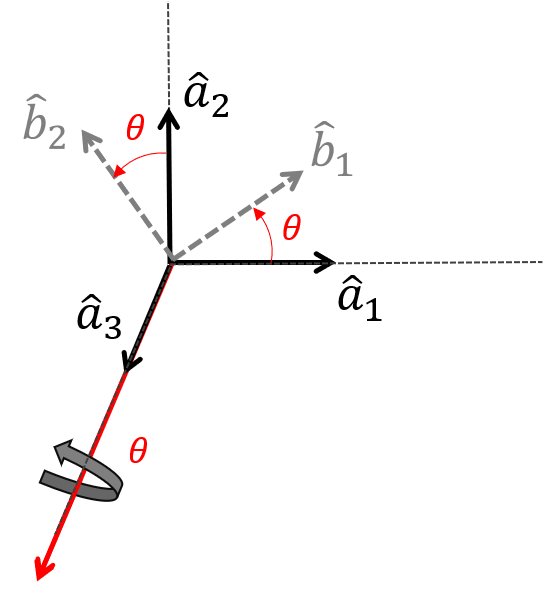
\includegraphics[width=0.30\textwidth]{r3.png}
				\label{fig:r3}}
				\hspace{+20pt}
				\subfloat[Vue de face]{
				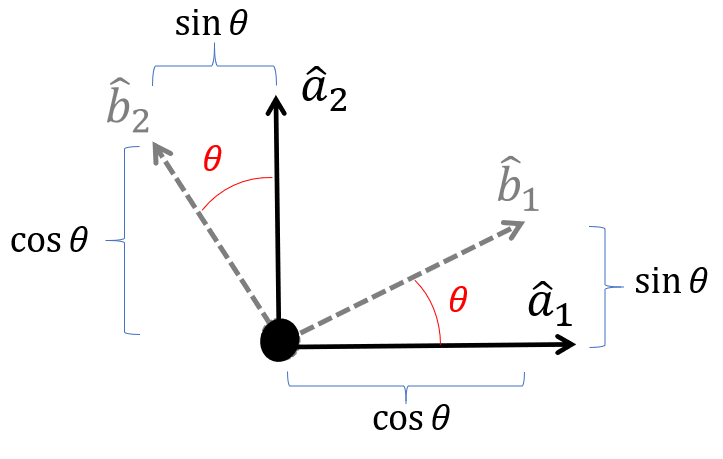
\includegraphics[width=0.40\textwidth]{r3v.png}
				\label{fig:r3v}}
        \caption{Rotation relative selon l'axe 3}
				\label{fig:r3vv}
\end{figure}
%%%%%%%%%%%%%%%%%%%%%%%%%%%%%%%%%%%%%%%%%%%%%%%%%%%%%%%%%%%%%%%%%
%

%%%%%%%%%%%%%%%%%%%%%%%%%%%%%%%%%%%
\paragraph{Rotation selon l'axe 2}
%
Si les bases vectorielles $a$ et $b$ ont une orientation relative décrite par une rotation d'un angle $\theta$ autour de l'axe 2, les vecteurs unitaires $\hat{a}_2$ et $\hat{b}_2$ sont égaux et, comme illustré à la figure \ref{fig:r2vv}, les quatre autres vecteurs unitaires ($\hat{a}_1$, $\hat{b}_1$, $\hat{a}_3$ et $\hat{b}_3$) sont dans le plan formé par l'axe 1 et l'axe 3. Les vecteurs unitaires sont reliés par des fonctions trigonométriques simples: 
%%%%%%%%%%%%%%%%%%%%
\begin{align}
\hat{b}_1 = c\theta \, \hat{a}_1 -s\theta \, \hat{a}_3 \quad\quad
\hat{b}_2 = \hat{a}_2 \quad\quad
\hat{b}_3 = s\theta \, \hat{a}_1 + c\theta \, \hat{a}_3
\label{eq:rot2vecuni}
\end{align}
%%%%%%%%%%%%%%%%%%%%
La matrice $^aR^b$ peut donc être formée grâce à la définition \eqref{eq:matricerotcol}:
%%%%%%%%%%%%%%%%%%%%
\begin{align}
\col{b}_1^a = \left[ \begin{array}{c} c\theta \\ 0 \\ -s\theta  \end{array} \right] \quad
\col{b}_2^a = \left[ \begin{array}{c} 0 \\ 1 \\ 0  \end{array} \right] \quad
\col{b}_3^a = \left[ \begin{array}{c} s\theta \\ 0 \\ c\theta  \end{array} \right]
\quad \Rightarrow \quad
^aR^b_2(\theta) = \left[ \begin{array}{c c c}
	c\theta  & 0 & s\theta \\
	0        & 1 & 0 \\
	-s\theta & 0 & c\theta 
\end{array}  \right]
\label{eq:rot2theta}
\end{align}
%%%%%%%%%%%%%%%%%%%
%
%%%%%%%%%%%%%%%%%%%%%%%%%%%%%%%%%%%%%%%%%%%%%%%%%%%%%%%%%%%%%%%
\begin{figure}[H]
        \centering
        \subfloat[3D]{
				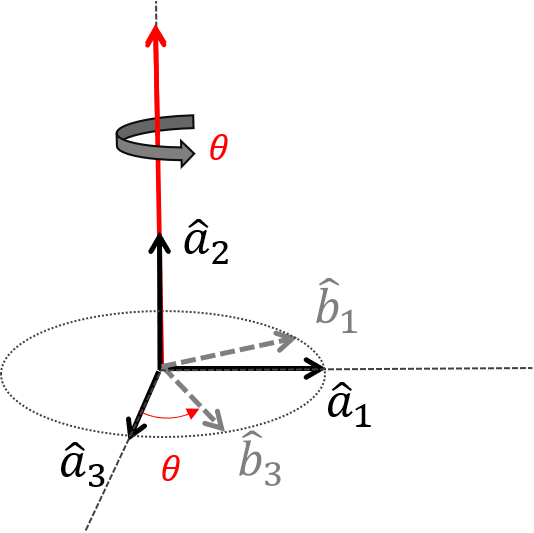
\includegraphics[width=0.30\textwidth]{r2.png}
				\label{fig:r2}}
				\hspace{+20pt}
				\subfloat[Vue de dessus]{
				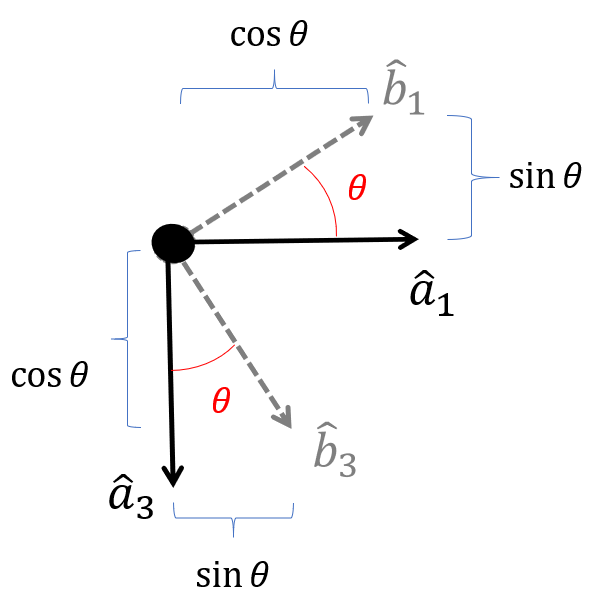
\includegraphics[width=0.30\textwidth]{r2v.png}
				\label{fig:r2v}}
        \caption{Rotation relative selon l'axe 2}
				\label{fig:r2vv}
\end{figure}
%%%%%%%%%%%%%%%%%%%%%%%%%%%%%%%%%%%%%%%%%%%%%%%%%%%%%%%%%%%%%%%%%
%


%%%%%%%%%%%%%%%%%%%%%%%%%%%%%%%%%%%
\paragraph{Rotation selon l'axe 1}
%
Si les bases vectorielles $a$ et $b$ ont une orientation relative décrite par une rotation d'un angle $\theta$ autour de l'axe 1, les vecteurs unitaires $\hat{a}_1$ et $\hat{b}_1$ sont égaux et, comme illustré à la figure \ref{fig:r3vv}, les quatre autres vecteurs unitaires ($\hat{a}_2$, $\hat{b}_2$, $\hat{a}_3$ et $\hat{b}_3$) sont dans le plan formé par l'axe 2 et l'axe 3. Les vecteurs unitaires sont reliés par des fonctions trigonométriques simples: 
%%%%%%%%%%%%%%%%%%%%
\begin{align}
\hat{b}_1 = \hat{a}_1 \quad\quad
\hat{b}_2 = c\theta \, \hat{a}_2 + s\theta \, \hat{a}_3 \quad\quad
\hat{b}_3 = -s\theta \, \hat{a}_2 + c\theta \, \hat{a}_3
\label{eq:rot1vecuni}
\end{align}
%%%%%%%%%%%%%%%%%%%%
La matrice $^aR^b$ peut donc être formée grâce à la définition \eqref{eq:matricerotcol}:
%%%%%%%%%%%%%%%%%%%%
\begin{align}
\col{b}_1^a = \left[ \begin{array}{c} 1 \\ 0 \\ 0  \end{array} \right] \quad
\col{b}_2^a = \left[ \begin{array}{c} 0 \\ c\theta \\ s\theta  \end{array} \right] \quad
\col{b}_3^a = \left[ \begin{array}{c} 0 \\ -s\theta \\ c\theta  \end{array} \right]
\quad \Rightarrow \quad
^aR^b_1(\theta) 
= \left[ \begin{array}{c c c}
	1 & 0 & 0 \\
	0 & c\theta  & -s\theta \\
	0 & s\theta & c\theta 
\end{array}  \right]
\label{eq:rot1theta}
\end{align}
%%%%%%%%%%%%%%%%%%%%
%
%%%%%%%%%%%%%%%%%%%%%%%%%%%%%%%%%%%%%%%%%%%%%%%%%%%%%%%%%%%%%%%
\begin{figure}[H]
        \centering
        \subfloat[3D]{
				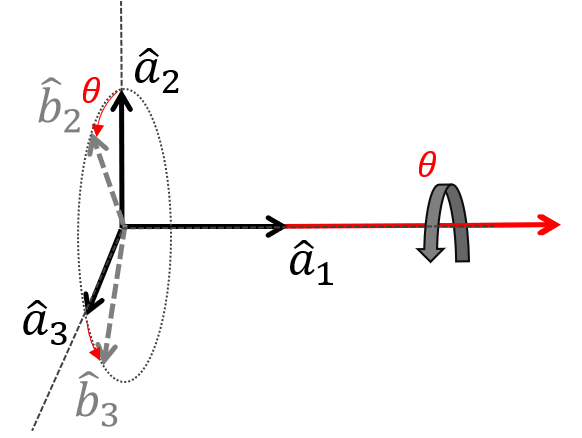
\includegraphics[width=0.30\textwidth]{r1.png}
				\label{fig:r1}}
				\hspace{+20pt}
				\subfloat[Vue de côté]{
				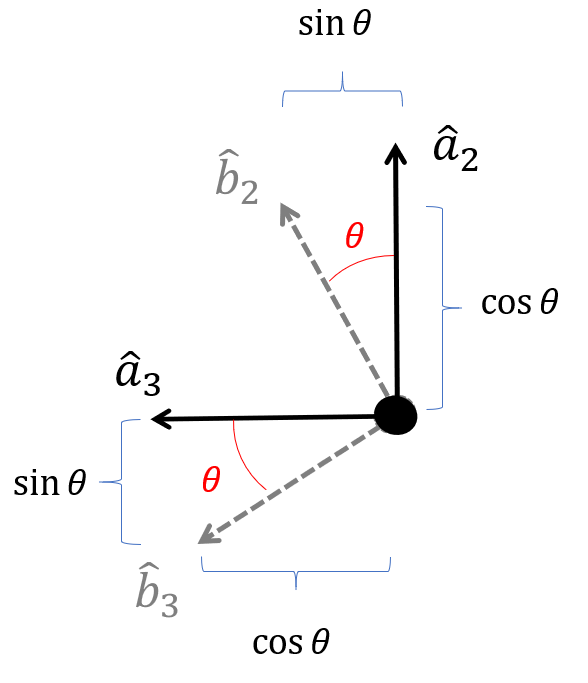
\includegraphics[width=0.30\textwidth]{r1v.png}
				\label{fig:r1v}}
        \caption{Rotation relative selon l'axe 1}
				\label{fig:r1vv}
\end{figure}
%%%%%%%%%%%%%%%%%%%%%%%%%%%%%%%%%%%%%%%%%%%%%%%%%%%%%%%%%%%%%%%%%


%%%%%%%%%%%%%%%%%%%%%%%%%%%%%%%%%%%%%%%%%%%%%%%%%%%%%%%%%%%%%
\subsection{Propriétés des matrices de rotation}

Cette section présente plusieurs propriétés des matrices de rotation qui sont utiles dans un contexte de changement de bases vectorielles.

%%%%%%%%%%%%%%%%%%%%%%%%%%%%%
\begin{property}[Norme des colonnes et rangés]

Les colonnes $\col{c}_i$ et les rangés $\col{r}_i$ d'une matrice de rotation ont une norme égale à 1:
%%%%%%%%%%%%%%%%%%%%%%%%%
\begin{align}
R &= 
\left[ \begin{array}{c c c} 
	\left[ \begin{array}{c} \\ \col{c}_1 \\  \\ \end{array}  \right] & \left[ \begin{array}{c} \\ \col{c}_2 \\  \\ \end{array}  \right] & \left[ \begin{array}{c} \\ \col{c}_3 \\  \\ \end{array}  \right]
\end{array} \right]
=
\left[ \begin{array}{c} 
\left[ \begin{array}{c c c} & \col{r}_1^T & \end{array} \right] \\[\medskipamount]
\left[ \begin{array}{c c c} & \col{r}_2^T & \end{array} \right] \\[\medskipamount]
\left[ \begin{array}{c c c} & \col{r}_3^T & \end{array} \right] 
\end{array} \right] 
\quad \Rightarrow \quad
(\col{c}_i)^T \col{c}_i = 1 \quad \& \quad (\col{r}_i)^T \col{r}_i = 1  \quad \forall i 
\end{align}
%%%%%%%%%%%%%%%%%%%%%%%%%
L’identité trigonométrique suivante est souvent utile pour ce type de calculs:
%%%%%%%%%%%%%%%%%%%%%%%%%
\begin{align}
\sin^2(\theta) + \cos^2(\theta) = 1
\end{align}
%%%%%%%%%%%%%%%%%%%%%%%%%
\end{property}


%%%%%%%%%%%%%%%%%%%%%%%%%%%%%
\begin{property}[Matrice identité]
Une matrice de rotation est réduite à une matrice identitée lorsque les bases vectorielle sont coïncidentes. Par exemple, pour les matrices de rotation élémentaires des équations \eqref{eq:rot3theta}, \eqref{eq:rot2theta} et \eqref{eq:rot1theta}, lorsque l'angle est égale à zéro, les matrices sont réduites à des matrices identités:
%%%%%%%%%%%%%%%%%%%%%%%%%%%%
\begin{align}
R_1( \theta ) = R_2( \theta ) = R_3( \theta ) = I_{3\times3} = 
\left[ \begin{array}{c c c}
	1 & 0 & 0 \\
	0 & 1 & 0 \\
	0 & 0 & 1 
\end{array}  \right]  \quad\text{si}\quad \theta = 0
\label{eq:rot3thetaident}
\end{align}
%%%%%%%%%%%%%%%%%%%%%
\end{property}


%%%%%%%%%%%%%%%%%%%%%%%%%%%%%
\begin{property}[Inversion]
Pour inverser la direction d'une opération de changement de base, il suffit de multiplier par l'inverse de la matrice de rotation:
%%%%%%%%%%%%%%%%%%%%%%%%
\begin{align}
\col{r}^a &= {}^aR^b \, \col{r}^b \\
({}^aR^b)^{-1} \, \col{r}^a &= ({}^aR^b)^{-1} \, {}^aR^b \, \col{r}^b  \\
({}^aR^b)^{-1} \, \col{r}^a &= \col{r}^b
\end{align}
%%%%%%%%%%%%%%%%%%%%%%%%%%%%%%
L'inversion d'une matrice de rotation est équivalente à inverser le signe de l'angle $\theta$ utilisé dans le calcul de la matrice, à prendre la transposée de la matrice et, en termes de notation, à inverser les bases:
%%%%%%%%%%%%%%%%%%%%%%%%
\begin{align}
R(\theta)^{-1} &= R(-\theta) \\
R^{-1} &= R^T \\
({}^bR^a)^{-1} &= {}^aR^b
\end{align}
%%%%%%%%%%%%%%%%%%%%%%%%%%%%%%
%\paragraph{Exercices de lecture}: Vérifiez ces propriétés pour la matrice exemple donnée à l'équation \eqref{eq:rot3theta}.
\end{property}

%%%%%%%%%%%%%%%%%%%%%%%%%%%%%
\begin{property}[Changements de base successifs]
Des changements de base successifs $a \rightarrow b \rightarrow c \rightarrow ... \rightarrow z$  peuvent être combinés en une seule matrice de rotation en multipliant les matrices de rotation intermédiaires par la gauche:
%%%%%%%%%%%%%%%%%%%
\begin{align}
{}^cR^a &=  {}^cR^b \, {}^bR^a \\
{}^dR^a &=  {}^dR^c \, {}^cR^b \, {}^bR^a \\
& \vdots \\
{}^zR^a &=  {}^zR^y \, {}^yR^x \, \hdots \, {}^cR^b \, {}^bR^a 
\end{align}
%%%%%%%%%%%%%%%%%%%
Notez que selon la notation utilisée dans ces notes, \textbf{les lettres des bases intermédiaires doivent être côte-à-côte dans les équations}, et la matrice de rotation totale conserve la première et la dernière base de la séquence dans le même ordre. Cette propriété découle des définitions, en combinant deux changements de base intermédiaires, une matrice totale peut être obtenue: 
%%%%%%%%%%%%%%%%%%%
\begin{align}
\left. \begin{array}{c}
\col{r}^b = {}^bR^a \col{r}^a \\  \col{r}^c = {}^cR^b \col{r}^b \\ \col{r}^c = {}^cR^a \col{r}^a 
\end{array} \right\} \quad \Rightarrow \quad \col{r}^c = \underbrace{{}^cR^b \,  {}^bR^a}_{ {}^cR^a } \col{r}^a \quad \Rightarrow \quad {}^cR^a  = {}^cR^b \,  {}^bR^a 
\end{align}
%%%%%%%%%%%%%%%%%%
\end{property}

%%%%%%%%%%%%%%%%%%%%%%%%%%%%%
\begin{property}[Non-commutativité]
Le produit des matrices de rotation n'est toutefois pas commutatif, sauf pour des petites rotations infinitésimales. L'ordre de multiplication des matrices est donc important et généralement:
%%%%%%%%%%%%%%%%%%%%%%
\begin{equation}
^cR^b \, ^bR^a \ne {}^bR^a \, ^cR^b
\end{equation} 
%%%%%%%%%%%%%%%%%%%%%%%
Une \textbf{exception à cette règle} est pour les rotations successives selon le même axe de rotation. Par exemple pour deux matrices de rotation élémentaires selon un axe $i$:
%%%%%%%%%%%%%%%%%%%%%%
\begin{equation}
R_i( \theta_1 ) R_i( \theta_2 )  = R_i( \theta_2 ) R_i( \theta_1 ) = R_i( \theta_1 + \theta_2 )
\end{equation} 
%%%%%%%%%%%%%%%%%%%%%%%
\end{property}


%%%%%%%%%%%%%%%%%%%%%%%%%%%%%%%%%%%%%%%%%%%%%%%%%%%%%%%%%%%%
\begin{example}[Réorganisation des vecteurs unitaires]
%
La figure \ref{fig:r_reorg} illustre deux bases vectorielles qui ont des vecteurs unitaires parallèles mais avec des directions et un ordre différents. Pour calculer la matrice de rotation associée $^bR^a$, la première étape est d'identifier la relation entre les vecteurs unitaires $\hat{a}_i$ et $\hat{b}_i$. 
%
%%%%%%%%%%%%%%%%%%%%%%%%%%%%%%%%%%%%%%%%%%%%%%%%%%%%%%%%%%%%%%%
\begin{figure}[H]
				%\vspace{-10pt}
        \centering
				\subfloat[Vue 3D]{
				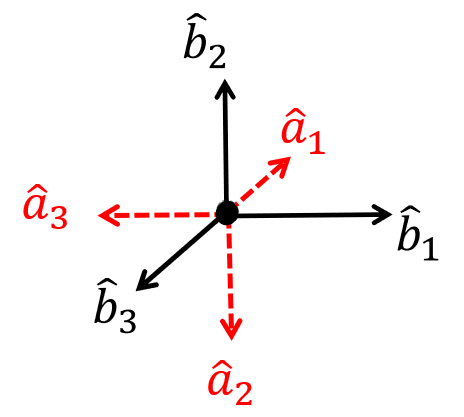
\includegraphics[width=0.25\textwidth]{r_reorg_3d}
				\label{fig:r_reorg_3}}
				%%%%
				\hspace{20pt}
				%%%%
        \subfloat[Vue de face]{
				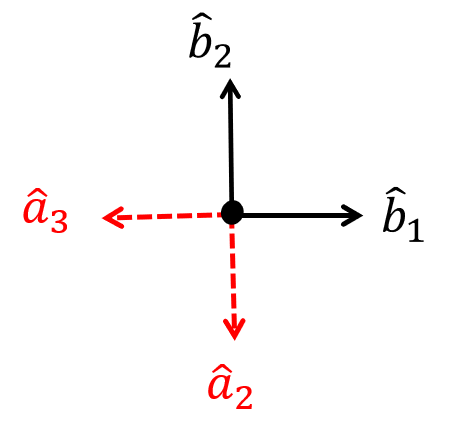
\includegraphics[width=0.25\textwidth]{r_reorg_face}
				\label{fig:r_reorg_face}}
				%%%%
				\hspace{20pt}
				%%%%
				\subfloat[Vue de dessus]{
				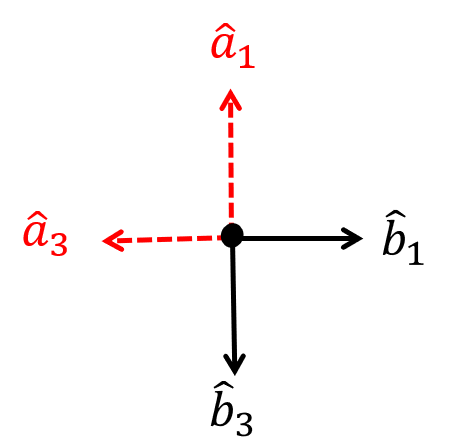
\includegraphics[width=0.25\textwidth]{r_reorg_top}
				\label{fig:r_reorg_top}}
        \caption{Réorganisation des directions des vecteurs unitaires}
				\label{fig:r_reorg}
\end{figure}
%%%%%%%%%%%%%%%%%%%%%%%%%%%%%%%%%%%%%%%%%%%%%%%%%%%%%%%%%%%%%%%%%
%
On peut constater que le vecteur unitaire $\hat{a}_1=-\hat{b}_3$, le vecteur unitaire $\hat{a}_2=-\hat{b}_2$ et le vecteur unitaire $\hat{a}_3=-\hat{b}_1$. Avec ces résultats il est possible d'assembler les vecteur-colonnes $\col{a}_i^b$:
%%
%%%%%%%%%%%%%
\begin{align}
\col{a}_1^b = \left[ \begin{array}{c} 0 \\ 0 \\ -1  \end{array} \right] \quad
\col{a}_2^b = \left[ \begin{array}{c} 0 \\ -1 \\ 0 \end{array} \right] \quad
\col{a}_3^b = \left[ \begin{array}{c} -1 \\ 0 \\ 0   \end{array} \right]
\end{align}
%%%%%%%%%%%%%
%%
Il est donc maintenant possible d'assembler la matrice de rotation $^bR^a$ basée sur l'équation \eqref{eq:matricerotcol}:
%%
%%%%%%%%%%%%
\begin{align}
^bR^a =\left[ \begin{array}{c c c}
	\col{a}_1^b  & \col{a}_2^b & \col{a}_3^b
\end{array}  \right]
= \left[ \begin{array}{c c c}
	0 & 0 & -1 \\
	0 & -1 & 0 \\
-1 & 0 & 0 
\end{array}  \right]
%\label{eq:rot3theta}
\end{align}
%%%%%%%%%%%%
\end{example}



%%%%%%%%%%%%%%%%%%%%%%%%%%%%%%%%%%%%%%%%%%%%%%%%%%%%%%%%%%%%
\begin{example}[Réorganisation des vecteurs unitaires et rotation selon un axe]
%
Un exemple de calcul d'une matrice de rotation $^bR^a$ est donné pour une base $a$ qui subit une révolution de $\theta$ degrés autour de l'axe $\hat{b}_3$ par rapport à une base $b$, mais ici avec des vecteurs unitaires qui sont définis avec des directions différentes, tel qu'illustré à la figure \ref{fig:rot3}, et ce n'est donc pas un cas de rotation élémentaire. Pour construire la matrice de rotation, la première étape est de dessiner les deux bases avec une origine commune, dans une configuration où la rotation $\theta$ est relativement faible (pour simplifier la visualisation). On peut constater que le vecteur unitaire $\hat{a}_1$ est aligné avec l'axe de rotation, donc indépendant de $\theta$ et toujours donné par $\hat{a}_1=-\hat{b}_3$. Ensuite, par inspection, il est possible d'exprimer chaque vecteur unitaire $\hat{a}_i$ comme une combinaison des vecteurs unitaires $\hat{b}_i$, avec des relations trigonométriques simples comme illustrés par les figures \ref{fig:rot3_a1} et \ref{fig:rot3_a2}. 
%
%%%%%%%%%%%%%%%%%%%%%%%%%%%%%%%%%%%%%%%%%%%%%%%%%%%%%%%%%%%%%%%
\begin{figure}[H]
				%\vspace{-10pt}
        \centering
				\subfloat[Base vectorielles $a$ et $b$]{
				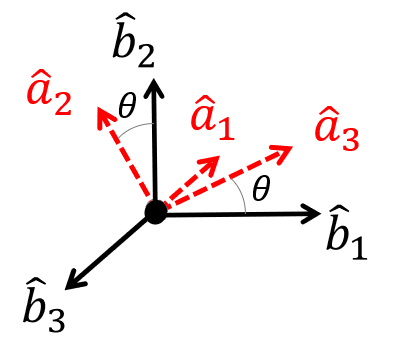
\includegraphics[width=0.25\textwidth]{rot3}
				\label{fig:rot3}}
				%%%%
				\hspace{20pt}
				%%%%
        \subfloat[Calcul de $\col{a}_3^b$]{
				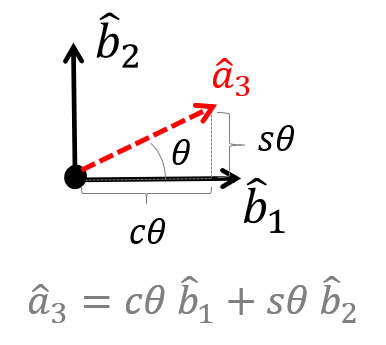
\includegraphics[width=0.25\textwidth]{rot3_a3}
				\label{fig:rot3_a1}}
				%%%%
				\hspace{20pt}
				%%%%
				\subfloat[Calcul de $\col{a}_2^b$]{
				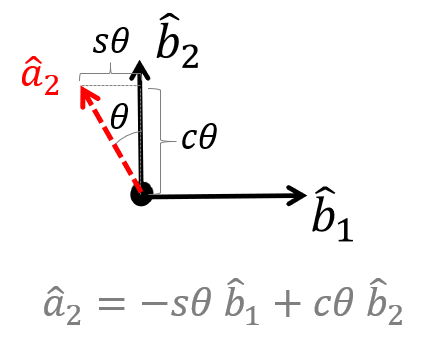
\includegraphics[width=0.25\textwidth]{rot3_a2}
				\label{fig:rot3_a2}}
        \caption{Rotation selon l'axe 3 et réorganisation des directions des vecteurs unitaires}
				\label{fig:rot3_a2}
\end{figure}
%%%%%%%%%%%%%%%%%%%%%%%%%%%%%%%%%%%%%%%%%%%%%%%%%%%%%%%%%%%%%%%%%
%
Avec ces résultats il est possible d'assembler les vecteur-colonnes $\col{a}_i^b$:
%%
%%%%%%%%%%%%%
\begin{align}
\col{a}_1^b = \left[ \begin{array}{c} 0 \\ 0 \\ -1  \end{array} \right] \quad
\col{a}_2^b = \left[ \begin{array}{c} -s\theta \\ c\theta \\ 0 \end{array} \right] \quad
\col{a}_3^b = \left[ \begin{array}{c} c\theta \\ s\theta \\ 0   \end{array} \right]
\end{align}
%%%%%%%%%%%%%
%%
Il est donc maintenant possible d'assembler la matrice de rotation $^bR^a$ basé sur l'équation \eqref{eq:matricerotcol}:
%%
%%%%%%%%%%%%
\begin{align}
^bR^a =\left[ \begin{array}{c c c}
	\col{a}_1^b  & \col{a}_2^b & \col{a}_3^b
\end{array}  \right]
= \left[ \begin{array}{c c c}
	0 & -s\theta & c\theta \\
	0 & c\theta & s\theta \\
-1 & 0 & 0 
\end{array}  \right]
%\label{eq:rot3theta}
\end{align}
%%%%%%%%%%%%
\end{example}

%%%%%%%%%%%%%%%%%%%%%%%%%%%%%%%%%%%%%%%%%%%%%%%%%%
\begin{example}[Calcul de la position globale de l'effecteur d'un robot]
\label{sec:exer-cinematique-base}
%
Dans cet exemple, le robot précédemment étudié (Figure \ref{fig:vecposunipro}) est ici analysé à nouveau mais cette fois avec l'aide des bases vectorielles. L'objectif est ici de calculer la position du point $D$ par rapport au point $A$ exprimée dans la base vectorielle $a$. Comme illustré à la figure \ref{fig:vecposbase1}, la première étape est de décrire la position qui doit être calculée en terme de vecteurs de position géométriques:
%%%%%%%%%%%%%%%%%%%%%%%%%%%%%%%%%%%
\begin{align}
\vec{r}_{D/A} &= \vec{r}_{D/C} + \vec{r}_{C/B} + \vec{r}_{B/A}
\end{align} 
%%%%%%%%%%%%%%%%%%%%%%%%%%%%%%%%%%%
Cette relation vectorielle peut ensuite être convertie en une équation matricielle entre les composantes dans une base $a$ fixe qui correspond aux axes selon lesquels la position doit être exprimée:
%%%%%%%%%%%%%%%%%%%%%%%%%%%%%%%%%%%
\begin{align}
\col{r}_{D/A}^a &= \col{r}_{D/C}^a + \col{r}_{C/B}^a + \col{r}_{B/A}^a
\label{eq:exaddbase}
\end{align} 
%%%%%%%%%%%%%%%%%%%%%%%%%%%%%%%%%%%
Ensuite, comme illustré à la Figure \ref{fig:vecposrot}, les différents vecteurs positions qui représentent chaque joint ont des composantes connues dans des bases vectorielles locales attachées aux différents liens rigides du robot:
%%%%%%%%%%%%%%%%%%%%%%%%%%%%%%%%%%%
\begin{align}
\col{r}_{B/A}^b = 
\left[ \begin{array}{c} 
l_1 \\ 0 \\ 0
\end{array} \right] 
\quad\quad
\col{r}_{C/B}^c = 
\left[ \begin{array}{c} 
0 \\ l_2 \\ 0
\end{array} \right]
\quad\quad
\col{r}_{D/C}^d = 
\left[ \begin{array}{c} 
0 \\ l_3 \\ 0
\end{array} \right] 
\end{align} 
%%%%%%%%%%%%%%%%%%%%%%%%%%%%%%%%%%%
Il est à noter que ces vecteur-colonnes qui utilisent les bases locales sont constants et indépendants des angles des joints car les base locales tournent avec les liens rigides. Il est ensuite possible de convertir ces vecteur-colonnes de positions dans la base $a$ par des opérations de changement de base avec les matrices de rotation appropriées:
%%%%%%%%%%%%%%%%%%%%%%%%%%%%%%%%%%%
\begin{align}
\col{r}_{D/C}^a = {}^aR^d \, \col{r}_{D/C}^d 
\quad \quad
\col{r}_{C/B}^a = {}^aR^c \, \col{r}_{C/B}^c
\quad \quad
\col{r}_{B/A}^a = {}^aR^b \, \col{r}_{B/A}^b
\end{align} 
%%%%%%%%%%%%%%%%%%%%%%%%%%%%%%%%%%%
Finalement, en substituant dans l'équation \eqref{eq:exaddbase}, l'équation matricielle nécessaire pour obtenir les composantes du vecteur position $\vec{r}_{D/A}$ exprimé avec la base $a$ est obtenue:
%%%%%%%%%%%%%%%%%%%%%%%%%%%%%%%%%%%
\begin{align}
\col{r}_{D/A}^a &= {}^aR^d \, \col{r}_{D/C}^d + {}^aR^c \, \col{r}_{C/B}^c + {}^aR^b \, \col{r}_{B/A}^b
\label{eq:ex333cinematique}
\end{align} 
%%%%%%%%%%%%%%%%%%%%%%%%%%%%%%%%%%%
Les matrices de rotation doivent ensuite être calculées pour solutionner cette équation.
%%%%%%%%%%%%%%%%%%%%%%%%%%%%%%%%%%%%%%%%%%%%%%%%%%%%%%%%%%%%%%%
\begin{figure}[H]
				%\vspace{-10pt}
        \centering
				\subfloat[Construction géométrique]{
				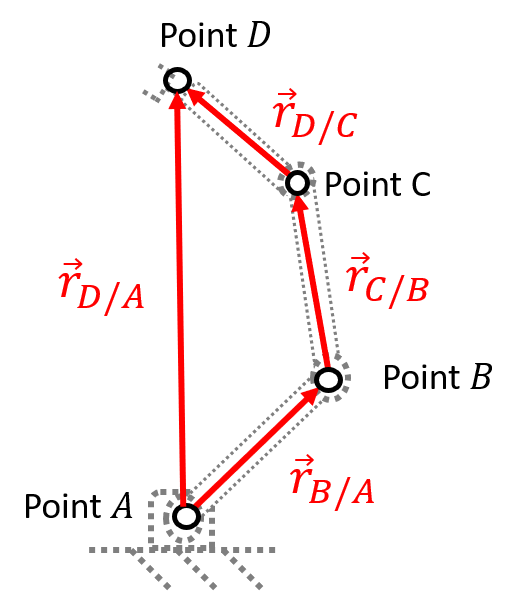
\includegraphics[width=0.30\textwidth]{vecposcons}
				\label{fig:vecposrot1}}
				%%%%
				\hspace{10pt}
				%%%%
        \subfloat[Bases vectorielles]{
				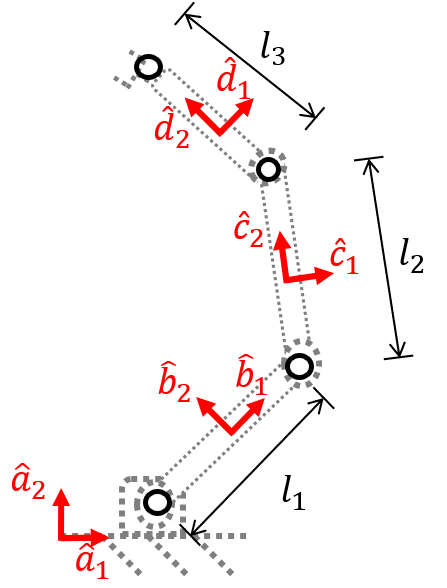
\includegraphics[width=0.27\textwidth]{vecposbase}
				\label{fig:vecposrot2}}
				%%%%
				\hspace{10pt}
				%%%%
        \subfloat[Angles]{
				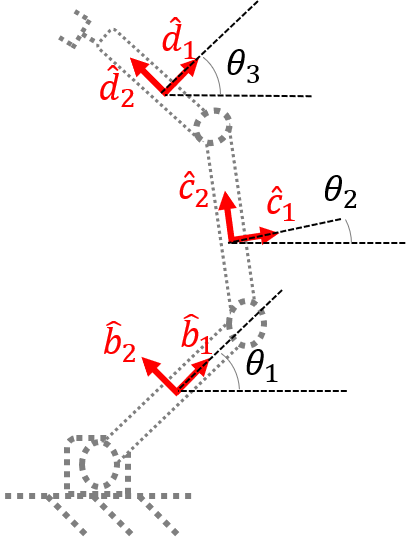
\includegraphics[width=0.27\textwidth]{vecposbaseangle}
				\label{fig:vecposrot3}}
        \caption{Utilisation des bases vectorielles pour les vecteurs de position}
				\label{fig:vecposrot}
\end{figure}
%%%%%%%%%%%%%%%%%%%%%%%%%%%%%%%%%%%%%%%%%%%%%%%%%%%%%%%%%%%%%%%%%
Grâce à une inspection des mouvements relatifs des bases vectorielles, comme illustrée à la figure \ref{fig:vecposrot2}, les matrices de rotation peuvent être calculées. Puisque le robot est planaire, les bases vectorielles $b$, $c$ et $d$ fixées aux pièces mobiles du robot ont tous une rotation relative autour de l'axe $\hat{a}_3$ par rapport à la base vectorielle fixe $a$, tel qu'illustré à la figure \ref{fig:exer-cinematique-base-rotation}.  
%
%%%%%%%%%%%%%%%%%%%%%%%%%%%%%%%%%%%%%%%%%%%%%%%%%%%%%%%%%%%%%%%
\begin{figure}[H]
				%\vspace{-10pt}
        \centering
        \subfloat[$^aR^b$]{
				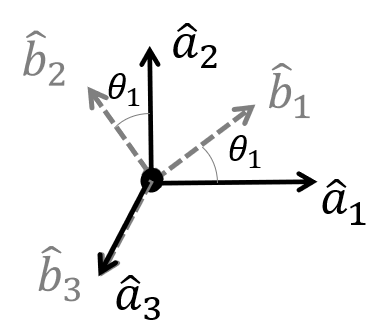
\includegraphics[width=0.20\textwidth]{baseext1}
				\label{fig:baseext1}}
				\hspace{10pt}
				\subfloat[$^aR^c$]{
				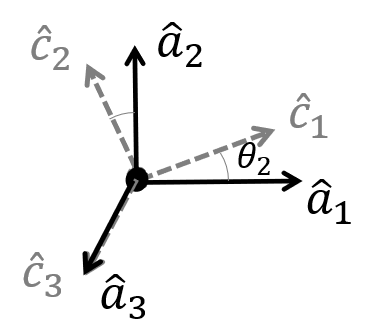
\includegraphics[width=0.20\textwidth]{baseext2}
				\label{fig:baseext2}}
				\hspace{10pt}
				\subfloat[$^aR^d$]{
				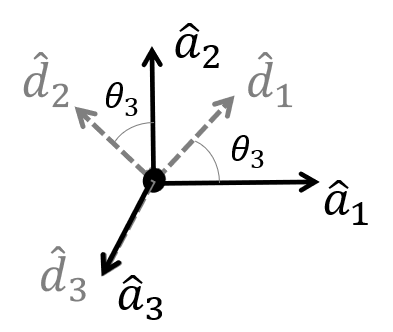
\includegraphics[width=0.20\textwidth]{baseext3}
				\label{fig:baseext3}}
        \caption{Calcul des matrices de rotation pour l'exemple \ref{sec:exer-cinematique-base}}
				\label{fig:exer-cinematique-base-rotation}
\end{figure}
%%%%%%%%%%%%%%%%%%%%%%%%%%%%%%%%%%%%%%%%%%%%%%%%%%%%%%%%%%%%%%%%%
%
En fonction des angles définis à la figure \ref{fig:vecposrot3}, les matrices de rotation sont donc toutes des matrices élémentaires de rotation autour de l'axe 3:
%%%%%%%%%%%%%%%%%%%%%%%%%%%%%%%%%%%
\begin{align}
{}^aR^b =
\left[ \begin{array}{c c c}
	c\theta_1 & -s\theta_1 & 0 \\
	s\theta_1 & c\theta_1 & 0 \\
	0 & 0 & 1 
\end{array}  \right]
\quad \quad
 {}^aR^c =
\left[ \begin{array}{c c c}
	c\theta_2 & -s\theta_2 & 0 \\
	s\theta_2 & c\theta_2 & 0 \\
	0 & 0 & 1 
\end{array}  \right]
\quad \quad
{}^aR^d =
\left[ \begin{array}{c c c}
	c\theta_3 & -s\theta_3 & 0 \\
	s\theta_3 & c\theta_3 & 0 \\
	0 & 0 & 1 
\end{array}  \right]
\end{align} 
%%%%%%%%%%%%%%%%%%%%%%%%%%%%%%%%%%%
Ces résultats peuvent donc être substitués dans l'équation matricielle qui avait été obtenue à l'exemple \ref{sec:exer-cinematique-base}:
%%%%%%%%%%%%%%%%%%%%%%%%%%%%%%%%%%%
\begin{align}
\col{r}_{D/A}^a &= {}^aR^d \, \col{r}_{D/C}^d + {}^aR^c \, \col{r}_{C/B}^c + {}^aR^b \, \col{r}_{B/A}^b
\label{eq:ex333cinematique-2}
\end{align} 
%%%%%%%%%%%%%%%%%%%%%%%%%%%%%%%%%%%
et on obtient l’expression précise qui permet de calculer la position du point $D$ par rapport au point de référence $A$ exprimée dans la base vectorielle $a$ en fonction des variables de distances $l_i$ et d'angles $\theta_i$:
%%%%%%%%%%%%%%%%%%%%%%%%%%%%%%%%%%%
\begin{align}
\col{r}_{D/A}^a &= \left[ \begin{array}{c c c}
	c\theta_3 & -s\theta_3 & 0 \\
	s\theta_3 & c\theta_3 & 0 \\
	0 & 0 & 1 
\end{array}  \right] \, \left[ \begin{array}{c} 
0 \\ l_3 \\ 0
\end{array} \right] + \left[ \begin{array}{c c c}
	c\theta_2 & -s\theta_2 & 0 \\
	s\theta_2 & c\theta_2 & 0 \\
	0 & 0 & 1 
\end{array}  \right] \, \left[ \begin{array}{c} 
0 \\ l_2 \\ 0
\end{array} \right]  + \left[ \begin{array}{c c c}
	c\theta_1 & -s\theta_1 & 0 \\
	s\theta_1 & c\theta_1 & 0 \\
	0 & 0 & 1 
\end{array}  \right] \, \left[ \begin{array}{c} 
l_1 \\ 0 \\ 0
\end{array} \right] \\
\col{r}_{D/A}^a &= \left[ \begin{array}{c}
-s\theta_3 l_3 - s\theta_2 l_2  + c\theta_1 l_1 \\
c\theta_3 l_3 + c\theta_2 l_2  + s\theta_1 l_1  \\
0
\end{array} \right]
\label{eq:robot2dpos}
\end{align} 
%%%%%%%%%%%%%%%%%
À noter que ici les angles $\theta_i$ sont tous des angles absolus qui représentent l'orientation des bases $b$, $c$ et $d$ du robot par rapport à la base fixe $a$ directement. Lorsqu'on contrôle un bras robotisé, c'est généralement les angles relatifs entre chacun des joints qui sont les variables mesurées et contrôlées. 

\paragraph{Exercice de lecture:}
La hauteur du robot correspond à la deuxième ligne de l'équation \eqref{eq:robot2dpos}, qui est la distance $\vec{r}_{D/A}$ selon le vecteur unitaire $\hat{a}_2$: 
%%%%%%%%%%%%%%%%%%%%%%%%%%%%%%%%%%%
\begin{align}
h = c\theta_3 l_3 + c\theta_2 l_2  + s\theta_1 l_1  
\end{align} 
%%%%%%%%%%%%%%%%%
Alternativement, à l'exemple \ref{sec:hauteurrobot}, l'équation suivante avait été obtenue pour la hauteur du robot:
%%%%%%%%%%%%%%%%%%%%%%%%%%%%%%%%%%%
\begin{align}
h &= l_1 \cos (\varphi_1) + l_2 \cos (\varphi_2) + l_3 \cos (\varphi_3)
\end{align} 
%%%%%%%%%%%%%%%%%%%%%%%%%%%%%%%%%%%
Trouvez la correspondance entre les angles $\theta_i$ et $\varphi_i$ et vérifiez que les deux expressions sont équivalentes.

\end{example}

%%%%%%%%%%%%%%%%%%%%%%%%%%%%%%%%%%%
\begin{example}[Distance projetée calculée avec les vecteur-colonnes]
%
Comme illustré à la figure \ref{fig:exprojcomp}, cet exemple démontre comment calculer la distance projetée $d_n$ d'un vecteur $\vec{r}_{C/A}$ selon un axe décrit par $\hat{n}$, connaissant les vecteur-colonnes de composantes:
%%%%%%%%%%%%%%%%%%%%%%%%%%%%%%%%%%%
\begin{align}
\col{r}_{C/B}^b = \left[ \begin{array}{c} x \\ y \\ z  \end{array} \right]
\quad\quad
\col{r}_{B/A}^a = \left[ \begin{array}{c} X \\ Y \\ Z  \end{array} \right]
\quad\quad
\col{n}^b       = \left[ \begin{array}{c} n_x \\ n_y \\ n_z  \end{array} \right]
\label{eq:disprojexdef}
\end{align} 
%%%%%%%%%%%%%%%%%%%%%%%%%%%%%%%%%%%
Premièrement, l'équation vectorielle de vecteurs géométriques de position est développée:
%%%%%%%%%%%%%%%%%%%%%%%%%%%%%%%%%%%
\begin{align}
\vec{r}_{C/A} = \vec{r}_{C/B} + \vec{r}_{B/A}
\end{align} 
%%%%%%%%%%%%%%%%%%%%%%%%%%%%%%%%%%%
pour ensuite effectuer le produit scalaire pour calculer la distance projetée:
%%%%%%%%%%%%%%%%%%%%%%%%%%%%%%%%%%%
\begin{align}
d_n = \vec{r}_{C/A} \bullet \hat{n} = (\vec{r}_{C/B} + \vec{r}_{B/A} ) \bullet \hat{n} 
\end{align} 
%%%%%%%%%%%%%%%%%%%%%%%%%%%%%%%%%%%
Deuxièmement, on choisi la base $b$ pour transformer la relation vectorielle en équation matricielle:
%%%%%%%%%%%%%%%%%%%%%%%%%%%%%%%%%%%
\begin{align}
d_n &= (\col{r}_{C/B}^b + \col{r}_{B/A}^b )^T \col{n}^b \\
d_n &= ( \col{r}_{C/B}^b )^T \col{n}^b + ( \col{r}_{B/A}^b )^T \col{n}^b
\end{align} 
%%%%%%%%%%%%%%%%%%%%%%%%%%%%%%%%%%%
Tous les vecteur-colonnes sont connus sauf le vecteur-colonne $\col{r}_{C/B}^b$, qui doit être substitué par $\col{r}_{C/B}^b = {}^bR^a \, \col{r}_{C/B}^a$ car les composantes de $\vec{r}_{C/B}$ sont connues seulement dans la base $a$. On obtient alors:
%%%%%%%%%%%%%%%%%%%%%%%%%%%%%%%%%%%
\begin{align}
d_n &= ( {}^bR^a \, \col{r}_{C/B}^a )^T \col{n}^b + ( \col{r}_{B/A}^b )^T \col{n}^b \\
d_n &= ( \col{n}^b )^T \, {}^bR^a \, \col{r}_{C/B}^a + ( \col{r}_{B/A}^b )^T \col{n}^b 
\end{align} 
%%%%%%%%%%%%%%%%%%%%%%%%%%%%%%%%%%%
et ce qui correspond en termes de composantes à l'équation:
%%%%%%%%%%%%%%%%%%%%%%%%%%%%%%%%%%%
\begin{align}
d_n &= \left[ \begin{array}{c c c}
	n_1^b & n_2^b & n_3^b  
\end{array}  \right]
\left[ \begin{array}{c c c}
	{}^bR^a_{11} & {}^bR^a_{12} & {}^bR^a_{13} \\ 
	{}^bR^a_{21} & {}^bR^a_{22} & {}^bR^a_{23} \\
	{}^bR^a_{31} & {}^bR^a_{32} & {}^bR^a_{33}
\end{array}  \right]
 \left[ \begin{array}{c} r_{C/B,1}^a \\ r_{C/B,2}^a \\ r_{C/B,3}^a  \end{array} \right]
+
\left[ \begin{array}{c c c}
	r_{B/A,1}^b & r_{B/A,2}^b & r_{B/A,3}^b  
\end{array}  \right]
 \left[ \begin{array}{c} n_1^b \\ n_2^b \\ n_3^b  \end{array} \right]
\end{align} 
%%%%%%%%%%%%%%%%%%%%%%%%%%%%%%%%%%%
si on substitue par les composantes connues définies à l'équation \eqref{eq:disprojexdef}:
%%%%%%%%%%%%%%%%%%%%%%%%%%%%%%%%%%%
\begin{align}
d_n &=
\left[ \begin{array}{c c c}
	n_x & n_y & n_z  
\end{array}  \right]
\left[ \begin{array}{c c c}
	{}^bR^a_{11} & {}^bR^a_{12} & {}^bR^a_{13} \\ 
	{}^bR^a_{21} & {}^bR^a_{22} & {}^bR^a_{23} \\
	{}^bR^a_{31} & {}^bR^a_{32} & {}^bR^a_{33}
\end{array}  \right]
 \left[ \begin{array}{c} x \\ y \\ z  \end{array} \right]
+
\left[ \begin{array}{c c c}
	X & Y & Z  
\end{array}  \right]
 \left[ \begin{array}{c} n_x \\ n_y \\ n_z  \end{array} \right]
\end{align} 
%%%%%%%%%%%%%%%%%%%%%%%%%%%%%%%%%%%
C'est donc cette équation qui devrait être programmée pour faire ce calcul numériquement sur un ordinateur.
%%%%%%%%%%%%%%%%%%%%%%%%%
\begin{figure}[H]
	\centering
		\includegraphics[width=0.50\textwidth]{exprojcomp.png}
	\caption{Exemple de calcul d'une distance projetée}
	\label{fig:exprojcomp}
\end{figure}
%%%%%%%%%%%%%%%%%%%%%%%%%%%
\end{example}

%%%%%%%%%%%%%%%%%%%%%%%%%%%%%%%%%%%%%%%%%%%%%%%%%%%%%%%%%%%%%%%%%%%%%%%%%%%%%%%%%%%%%%%%%%%%%%%%%%%%%%%%%%%%%%%%%%%%%%%%%%%%%%%%%%%%%%%%%%%%%%%%%%%%%%%%%%
\newpage
\section{Coordonnées dans un repère et transformations homogènes}
\label{sec:repere}

En robotique, il est souvent utile de placer un point de référence ainsi qu'une base vectorielle sur chaque corps rigide du robot. Bien qu'on peut travailler avec des points de référence et des bases vectorielles de façon indépendante, il est souvent pratique de les jumeler en paires puisqu'il faut ces deux types de références pour exprimer des coordonnées. \textbf{La combinaison d'un point d'origine et d'une base vectorielle est appelée repère dans ces notes}, le terme \textit{Frame} est généralement utilisé en anglais. Un repère $A$ dans ces notes fait donc référence à la fois à un point d'origine $A_o$ et à une base vectorielle $a$ qui consiste des trois vecteurs unitaires $\{ \hat{a}_1, \hat{a}_2, \hat{a}_3 \}$. Autrement dit, on appellera \textit{repère} $A$ le repère formé par l'ensemble $\{ A_o, \hat{a}_1, \hat{a}_2, \hat{a}_3 \}$. 
%%%%%%%%%%%%%%%%%%%%%%%%%%%%%%%%%%%%%%%%%%%%%%%%%%%%%%%%%%%%%%%%%%%%%%%%%%%%%
\begin{figure}[H]
	\centering
		\includegraphics[width=0.45\textwidth]{repere}
	\caption{Système de coordonnées cartésiennes $(x,y,z)$ basé sur le repère $\{A_o,\hat{a}_1,\hat{a}_2,\hat{a}_3\}$}
	\label{fig:repere}
\end{figure}
%%%%%%%%%%%%%%%%%%%%%%%%%%%%%%%%%%%%%%%%%%%%%%%%%%%%%%%%%%%%%%%%%%%%%%%%%%%%%%%

Comme illustré à la figure \ref{fig:repere}, les coordonnées cartésiennes ($x$, $y$, $z$) d'un point $P$ correspondent directement aux composantes du vecteur position avec comme origine l'intersection des axes du système de coordonnées (le point $A_o$) et exprimé dans une base vectorielle $a$ alignée sur les axes du système de coordonnées:
%%%%%%%%%%%%%%%%%%%%%%%%%%%%%%%%%%%
\begin{align}
\col{r}_{P/A_o}^a = \left[ \begin{array}{c} 
x \\ y \\ z
\end{array} \right]   \quad \Leftrightarrow \quad
\vec{r}_{P/A_o} = x \, \hat{a}_{1} + y \, \hat{a}_{2} + z \, \hat{a}_{3}
\end{align} 
%%%%%%%%%%%%%%%%%%%%%%%%%%%%%%%%%%%
Un système de coordonnées est toujours implicitement attaché à un repère, même s'il n'est pas explicitement défini. L'ensemble de l'origine des axes et des vecteurs unitaires alignés sur ces axes forment un repère. 

%Pour modéliser un bras robotique, il est utile de définir un repère sur chaque corps rigides, car les coordonnées des différents points d’intérêts sont constantes quand elles sont exprimées dans des repères locaux.

\video{Les repères et les matrices de transformation}{https://youtu.be/yTPA1R8b8XE}


%%%%%%%%%%%%%%%%%%%%%%%%%%%%%%%%%%%%%%%%%%%%%%%%%%%%%%%%%%%%%%%%%
\subsection{Changement de repère}
\label{sec:repchan}

Un changement de repère implique deux opérations: \textbf{1)} un changement de l'origine utilisée pour les vecteurs de position et \textbf{2)} un changement de la base vectorielle utilisée pour exprimer les composantes de ce vecteur position. 
%%%%%%%%%%%%%%%%%%%%%%%%%%%%%%%%%%%%%%%%%%%%%%%%%%%%%%%%%%%%%%%
\begin{figure}[htpb]
				%\vspace{-10pt}
        \centering
				\subfloat[Deux systèmes de coordonnées]{
				\includegraphics[width=0.40\textwidth]{repchaA}
				\label{fig:repchaA}}
				%%%%
				\hspace{10pt}
				%%%%
				\subfloat[Construction géométrique]{
				\includegraphics[width=0.40\textwidth]{repchaB}
				\label{fig:repchaB}}
        \caption{Changement du repère $\{B_o,\hat{b}_1,\hat{b}_2,\hat{b}_3\}$ vers  le repère $\{A_o,\hat{a}_1,\hat{a}_2,\hat{a}_3\}$}
				\label{fig:repcha}
\end{figure}
%%%%%%%%%%%%%%%%%%%%%%%%%%%%%%%%%%%%%%%%%%%%%%%%%%%%%%%%%%%%%%%%%
Comme illustré à la figure \ref{fig:repcha} pour une transformation d'un repère B vers un repère A, les coordonnées cartésiennes d'un point $C$ correspondent au vecteur-colonne $\col{r}_{C/B_o}^b$ dans le repère B et au vecteur-colonne $\col{r}_{C/A_o}^a$ dans le repère A:
%%%%%%%%%%%%%%%%%%%%%%%%%%%%%%%%%%%
\begin{align}
\col{r}_{C/B_o}^b = 
\left[ \begin{array}{c} 
x \\ y \\ z
\end{array} \right]  \quad \quad
\col{r}_{C/A_o}^a = 
\left[ \begin{array}{c} 
X \\ Y \\ Z
\end{array} \right] 
\end{align} 
%%%%%%%%%%%%%%%%%%%%%%%%%%%%%%%%%%%
Pour effectuer la transformation des coordonnées ($x$, $y$, $z$) vers les coordonnées ($X$, $Y$, $Z$), la première étape est de construire la relation vectorielle qui relie les trois points:
%%%%%%%%%%%%%%%%%%%%%%%%%%%%%%%%%%%
\begin{align}
\vec{r}_{C/A_o}   &= \vec{r}_{C/B_o}  + \vec{r}_{B_o/A_o} 
\end{align} 
%%%%%%%%%%%%%%%%%%%%%%%%%%%%%%%%%%%
et ensuite il suffit de tout exprimer ces vecteurs dans la base $a$ pour effectuer l'addition:
%%%%%%%%%%%%%%%%%%%%%%%%%%%%%%%%%%%
\begin{align}
\col{r}_{C/A_o}^a &=         \col{r}_{C/B_o}^a  + \col{r}_{B_o/A_o}^a  \\
\col{r}_{C/A_o}^a &= {}^aR^b \col{r}_{C/B_o}^b  + \col{r}_{B_o/A_o}^a 
\label{eq:reperechang}
\end{align} 
%%%%%%%%%%%%%%%%%%%%%%%%%%%%%%%%%%%
ce qui correspond en termes de coordonnées à: 
%%%%%%%%%%%%%%%%%%%%%%%%%%%%%%%%%%%
\begin{align}
\left[ \begin{array}{c} 
X \\ Y \\ Z
\end{array} \right]  &=  
 {}^aR^b
\left[ \begin{array}{c} 
x \\ y \\ z
\end{array} \right] + \col{r}_{B_o/A_o}^a 
\end{align} 
%%%%%%%%%%%%%%%%%%%%%%%%%%%%%%%%%%%
Un changement de base est nécessaire puisque que le vecteur $\vec{r}_{C/B_o}$ est connu dans la base vectorielle $b$. Donc les informations nécessaires pour effectuer la transformation sont: \textbf{1)} les composantes $\col{r}_{B_o/A_o}^a$ du vecteur position qui relie les origines $A_o$ et $B_o$ et 2\textbf{)} la matrice de rotation $^aR^b$ qui donne l'orientation relative des bases vectorielles $a$ et $b$. 

L'\textbf{opération inverse} s'obtient à partir de l'équation \eqref{eq:reperechang}, d'abord on soustrait le vecteur translation $\col{r}_{B_o/A_o}^a$ et on multiplie par la gauche l'inverse de la matrice de rotation pour obtenir:
%%%%%%%%%%%%%%%%%%%%%%%%%%%%%%%%%%%
\begin{align}
\col{r}_{C/B_o}^b &= {}^bR^a \; \col{r}_{C/A_o}^a - {}^bR^a \; \col{r}_{B_o/A_o}^a 
\label{eq:reperechanginv}
\end{align} 
%%%%%%%%%%%%%%%%%%%%%%%%%%%%%%%%%%%
ce qui correspond en termes des coordonnées à: 
%%%%%%%%%%%%%%%%%%%%%%%%%%%%%%%%%%%
\begin{align}
\left[ \begin{array}{c} 
x \\ y \\ z
\end{array} \right]  &=  
 {}^bR^a
\left[ \begin{array}{c} 
X \\ Y \\ Z
\end{array} \right] + {}^bR^a \; \col{r}_{B_o/A_o}^a 
\end{align} 
%%%%%%%%%%%%%%%%%%%%%%%%%%%%%%%%%%%




%%%%%%%%%%%%%%%%%%%%%%%%%%%%%%%%%%%%%%%%%%%%%%%%%%
\subsection{Coordonnées et transformations homogènes}
\label{sec:coordhomo}

Dans les logiciels de cinématique et de graphique, les opérations de changement de repère peuvent être très fréquentes. Il existe une méthode standard pour combiner l'opération d'addition vectorielle et la multiplication avec la matrice de rotation en une seule opération équivalente qui consiste à multiplier une matrice de transformation $4\times4$ notée $^AT^B$, avec un vecteur-colonne $4\times1$ de \textit{coordonnées homogènes}. Les coordonnées homogènes sont tout simplement les coordonnées cartésiennes pour les trois premières composantes et la valeur 1 pour la quatrième composante. 

Le changement de repère décrit à la section \ref{sec:repchan} correspond alors à l'opération suivante:
%%%%%%%%%%%%%%%%%%%%%%%%%%%%%%%%%%%
\begin{align}
\left[ \begin{array}{c} 
\col{r}_{C/A_o}^a \\ 1
\end{array} \right] 
= 
\underbrace{
\left[ \begin{array}{c c } 
^aR^b & \col{r}_{B_o/A_o}^a \\ 0 \; 0 \; 0 & 1
\end{array} \right] 
}_{^AT^B}
\left[ \begin{array}{c} 
\col{r}_{C/B_o}^b \\ 1
\end{array} \right] 
\label{eq:homo1}
\end{align} 
%%%%%%%%%%%%%%%%%%%%%%%%%%%%%%%%%%%
ce qui correspond en termes de coordonnées à:
%%%%%%%%%%%%%%%%%%%%%%%%%%%%%%%%%%%
\begin{align}
\left[ \begin{array}{c} 
X \\ Y \\ Z \\ 1
\end{array} \right] 
= 
\underbrace{
\left[ \begin{array}{c c } 
^aR^b & \col{r}_{B_o/A_o}^a \\ 0 \; 0 \; 0 & 1
\end{array} \right] 
}_{^AT^B}
\left[ \begin{array}{c} 
x \\ y \\ z \\ 1
\end{array} \right] 
\label{eq:homo2}
\end{align} 
%%%%%%%%%%%%%%%%%%%%%%%%%%%%%%%%%%%
Les trois premières rangés des équations matricielles \eqref{eq:homo1} et \eqref{eq:homo2} correspondent exactement à l'équation \eqref{eq:reperechang}, et la dernière ligne correspond simplement à une équation 1=1. Les transformations homogènes c'est donc rien de fondamentalement nouveau, mais une astuce bien utile dans un contexte de programmation pour grouper deux opérations en une seule. %D'autre types d'opérations peuvent aussi être exprimés sous la forme d'une multiplication d'une matrice de transformation 4x4 sur un vecteur-colonne 4x1 de coordonnées homogènes. 

Si on substitut les définitions, la matrice de transformation peut être définie directement en termes de vecteurs de vecteurs unitaires et du vecteur géométrique qui définie la translation d'une origine à l'autre:
%%%%%%%%%%%%%%%%%%%%%%%%%%%%%%%%%%%
\begin{align}
{}^AT^B &= 
\left[ \begin{array}{c c } 
^aR^b & \col{r}_{B_o/A_o}^a \\ 0 \; 0 \; 0 & 1
\end{array} \right] 
=
\left[ \begin{array}{c c c c} 
\hat{a}_1 \bullet \hat{b}_1  &  \hat{a}_1 \bullet \hat{b}_2  &  \hat{a}_1 \bullet \hat{b}_3 & \hat{a}_1 \bullet \vec{r}_{B_o/A_o} \\
\hat{a}_2 \bullet \hat{b}_1  &  \hat{a}_2 \bullet \hat{b}_2  &  \hat{a}_2 \bullet \hat{b}_3 & \hat{a}_2 \bullet \vec{r}_{B_o/A_o}\\
\hat{a}_3 \bullet \hat{b}_1  &  \hat{a}_3 \bullet \hat{b}_2  &  \hat{a}_3 \bullet \hat{b}_3 & \hat{a}_3 \bullet \vec{r}_{B_o/A_o} \\
0 & 0 & 0 & 1
\end{array} \right] 
\label{eq:transformationdef}
\end{align} 
%%%%%%%%%%%%%%%%%%%%%%%%%%%%%%%%%%%


L'\textbf{opération inverse} de changement de repère avec les coordonnées homogènes est formée par:
%%%%%%%%%%%%%%%%%%%%%%%%%%%%%%%%%%%
\begin{align}
\left[ \begin{array}{c} 
\col{r}_{C/B_o}^b \\ 1
\end{array} \right] 
= 
\underbrace{
\left[ \begin{array}{c c } 
^bR^a & - ^bR^a \, \col{r}_{B_o/A_o}^a \\ 0 \; 0 \; 0 & 1
\end{array} \right] 
}_{ ({}^AT^B)^{-1} }
\left[ \begin{array}{c} 
\col{r}_{C/A_o}^a \\ 1
\end{array} \right] 
\end{align} 
%%%%%%%%%%%%%%%%%%%%%%%%%%%%%%%%%%%
Comme pour les matrices de rotation l'inverse de la matrice de transformation correspond à inverser les repères avec la notation utilisée:
%%%%%%%%%%%%%%%%%%%%%%%%%%%%%%%%%%%
\begin{align}
({}^AT^B)^{-1}= {}^BT^A
\end{align} 
%%%%%%%%%%%%%%%%%%%%%%%%%%%%%%%%%%%

Dernièrement, les \textbf{changements de repères successifs} $A \rightarrow B \rightarrow C \rightarrow ... \rightarrow Z$  peuvent être combinés en une seule matrice de transformation en multipliant les matrices de transformation intermédiaires par la gauche:
%%%%%%%%%%%%%%%%%%%%%%%%%%%%%%%%%%%
\begin{align}
{}^CT^A &=  {}^CT^B \, {}^BT^A \\
{}^DT^A &=  {}^DT^C \, {}^CT^B \, {}^BT^A \\
& \vdots \nonumber \\
{}^ZT^A &= {}^ZT^Y \, {}^YT^X \, ... \, {}^CT^B \,  {}^BT^A 
\end{align} 
%%%%%%%%%%%%%%%%%%%%%%%%%%%%%%%%%%%
Avec la notation utilisée dans ces notes, \textbf{les lettres des repères intermédiaires doivent être côte-à-côte dans les équations}, et la matrice de transformation totale conserve le premier et le dernier repère de la séquence dans le même ordre. 




%%%%%%%%%%%%%%%%%%%%%%%%%%%%%%%%%%%%%%%%%%%%%%%%%%%%%%%%%%%%%%%%%
\newpage
\section{Représentation de la pose d'un corps rigide}
\label{sec:corps}

De façon générale, six variables sont nécessaires pour définir la positon d'un corps rigide par rapport à un repère, trois pour décrire la translation et trois pour décrire l'orientation. Pour un corps rigide sans aucune contrainte, par exemple un avion en vol, le nombre de DDL est donc de six. 

%%%%%%%%%%%%%%%%%%%%%%%%%%%%%%%%%%%%%%%%%%%%%%%%%%%%%%%%%%%%%%%%%%%%%%%%%%%%%
\begin{figure}[H]
	\centering
		\includegraphics[width=0.95\textwidth]{rigid.png}
	\caption{Représentation de la pose d'un corp rigide}
	\label{fig:rigid}
\end{figure}
%%%%%%%%%%%%%%%%%%%%%%%%%%%%%%%%%%%%%%%%%%%%%%%%%%%%%%%%%%%%%%%%%%%%%%%%%%%%%%%

\video{Pose (position et orientation) d'un corps rigide}{https://youtu.be/wrw4T8OE36U}

\paragraph{Translation:}
%
Les trois DDL de translation peuvent être représentés par un vecteur position qui a comme origine un point fixe $A$ et comme cible un point arbitraire $B$ sur le corps rigide. Ce vecteur position $\vec{r}_{B/A}$, est typiquement représenté avec trois coordonnées cartésiennes ($x$, $y$, $z$) qui utilisent une base vectorielle fixe $a$:
%%%%%%%%%%%%%%%%%%%
\begin{equation}
\col{r}_{B/A}^a = \left[ \begin{array}{c} x \\  y \\ z  \end{array} \right]
\quad \Leftrightarrow  \quad 
\vec{r}_{B/A} = x \, \vec{a}_1 + y \, \vec{a}_2 + z \, \vec{a}_3
\end{equation} 
%%%%%%%%%%%%%%%%%%%%

\paragraph{Orientation:}
%
Ensuite, même avec un point défini dans l'espace par un vecteur translation, un corps rigide a plusieurs orientations possibles. Pour définir l'orientation, une autre base vectorielle $b$ attachée au corps rigide doit être utilisée. L'orientation d'un corps rigide est alors représentée par la direction des vecteurs unitaires $\hat{b}_i$, qui peuvent être représentés par leurs composantes dans la base fixe $a$. Les trois vecteur-colonnes $\col{b}_i^a$ de trois composantes peuvent être regroupés sous la forme d'une matrice de rotation, comme il a été discuté à la section \ref{sec:changematrice} dans le contexte des changements de base:
%%%%%%%%%%%%%%%%%%%
\begin{equation}
^aR^b = \left[ \begin{array}{ c c c } \col{b}_1^a &  \col{b}_2^a & \col{b}_3^a  \end{array} \right] = R(\phi,\theta,\psi)
\end{equation} 
%%%%%%%%%%%%%%%%%%%%

Malgré les neuf composants d'une matrice de rotation, puisque les vecteurs $\hat{b}_i$ sont unitaires et orthogonaux seulement trois variables suffisent pour la définir; il y a un total de neuf composantes et six équations de contraintes, voir les équations \eqref{eq:unit} et \eqref{eq:ortho}. Il est donc possible de paramétrer la matrice $^aR^b$ avec trois variables, par exemple trois angles $\phi$, $\theta$ et $\psi$, sans limiter les orientations possibles. On appelle trois angles qui paramétrisent une matrice de rotation des angles de Euler, diverses conventions de paramétrisation sont possibles et c'est le sujet de la section \ref{sec:angeuler}. Selon la situation, d'autres représentations alternatives aux matrices de rotation et aux angles de Euler peuvent aussi être utiles, chaque représentation a ses avantages et inconvénients. La section \ref{sec:rotaxe} présente la représentation axe-angle et la section \ref{sec:quaternions} présente les quaternions. 

%\paragraph{Note:} L'orientation d'un corps rigide est aussi parfois appelée \textit{attitude}, typiquement dans le domaine de l'aérospatiale, ou bien \textit{position angulaire}.

\paragraph{Pose:}
La pose d'un corps rigide, c'est la combinaison de sa translation et de son orientation. Il est possible d'utiliser des représentations indépendantes pour la translation et l'orientation, mais alternativement on peut regrouper une matrice de rotation (pour représenter l'orientation) et un vecteur-colonne (pour représenter la translation)  sous la forme d'une matrice de transformation 4x4, qui relie le repère $\{A_o,\hat{a}_1,\hat{a}_2,\hat{a}_3\}$ formé par le point fixe et la base fixe, au repère $\{B_o,\hat{b}_1,\hat{b}_2,\hat{b}_3\}$ formé par le point mobile et la base mobile attachés au corps rigide. Cette matrice peut alors être paramétrée par 6 variables qui représent tous les DDL du corps rigide:
%%%%%%%%%%%%%%%%%%%
\begin{equation}
^{A}T^B(x,y,z,\phi,\theta,\psi) = \left[ \begin{array}{c c}
	^aR^b  & \col{r}^a_{B/A} \\ 0 \; 0 \; 0 & 1
\end{array}  \right] = 
\left[ \begin{array}{c c}
\left[	\begin{array}{c} \\  R(\phi,\theta,\psi) \\ \\ \end{array} \right] & \left[ \begin{array}{c} x \\ y \\ z \end{array} \right] \\  \begin{array}{ccc} 0 & 0 & 0 \end{array}   &  1 
\end{array}  \right] 
\end{equation} 
%%%%%%%%%%%%%%%%%%%%

La matrice de transformation $^{A}T^B$ a donc deux fonctions: \textbf{1)} elle peut être utilisée pour effectuer des changements de repères comme vue à la section \ref{sec:coordhomo}, et \textbf{2)} elle peut aussi être utilisée pour représenter la pose d'un repère $B$ (donc aussi la pose du corps rigide sur lequel il est attaché) relativement à un repère $A$.  


%%%%%%%%%%%%%%%%%%%%%%%%%%%%%%%%%%%%%%%%%%%%%%%%%%%%%%%%%%%%%%%%%%%%%%%%%%%%%%%
\subsection{Angles de Euler}
\label{sec:angeuler}

Une matrice de rotation arbitraire peut être paramétrée avec trois variables. La méthode la plus simple pour y parvenir est de construire une matrice de rotation comme une multiplication de trois matrices élémentaires. Par exemple, l'orientation arbitraire d'une base vectorielle $d$ par rapport à une base vectorielle $a$ peut être décrite par les angles $( \phi, \theta, \psi)$, avec la convention 3-1-3:
%%%%%%%%%%%%%%%%%%%
\begin{align}
{}^aR^d(\phi,\theta,\psi) &= R_3(\phi) \, R_1(\theta) \, R_3(\psi) \\
{}^aR^d(\phi,\theta,\psi) &= 
\left[ \begin{array}{c c c}
	c\phi & -s\phi & 0 \\
	s\phi & c\phi & 0 \\
	0 & 0 & 1 
\end{array}  \right]
\left[ \begin{array}{c c c}
	1 & 0 & 0 \\
	0 & c\theta  & -s\theta \\
	0 & s\theta & c\theta 
\end{array}  \right]
\left[ \begin{array}{c c c}
	c\psi & -s\psi & 0 \\
	s\psi & c\psi & 0 \\
	0 & 0 & 1 
\end{array}  \right] \\
{}^aR^d(\phi,\theta,\psi) &= 
\left[ \begin{array}{c c c}
	 + c\phi \, c\psi - s\phi\,c\theta\,c\psi  & - c\phi \, s\psi - s\phi \, c\theta c\psi  & + s\phi \, s\theta  \\
	 + s\phi \, c\psi + c\phi\,c\theta\,c\psi  & - s\phi \, s\psi + c\phi \, c\theta c\psi  & - c\phi \, s\theta  \\
	 + s\theta \, s\psi                        & + s\theta \, c\psi                          & + c\theta 
\end{array}  \right]
\end{align} 
%%%%%%%%%%%%%%%%%%%%
Cette matrice peut être interprétée comme une suite de trois rotations, avec des bases vectorielles intermédiaires, illustrées à la figure \ref{fig:euler}. 
%%%%%%%%%%%%%%%%%%%%%%%%%%%%%%%%%%%%%%%%%%%%%%%%%%%%%%%%%%%%%%%
\begin{figure}[H]
				%\vspace{-10pt}
        \centering
        \subfloat[${}^aR^b=R_3(\phi)$]{
				\includegraphics[width=0.28\textwidth]{euler1}
				\label{fig:euler1}}
				\subfloat[${}^bR^c=R_1(\theta)$]{
				\includegraphics[width=0.30\textwidth]{euler2}
				\label{fig:euler2}}
				\subfloat[${}^cR^d=R_3(\psi)$]{
				\includegraphics[width=0.33\textwidth]{euler3}
				\label{fig:euler3}}
        \caption{Angles de Euler avec la convention 3-1-3: toutes les orientations possibles de la base $d$ peuvent être décrites par la matrice de rotation ${}^aR^d(\phi,\theta,\psi) = R_3(\phi)R_1(\theta)R_3(\psi)$ paramétrisée avec trois angles.}
				\label{fig:euler}
\end{figure}
%%%%%%%%%%%%%%%%%%%%%%%%%%%%%%%%%%%%%%%%%%%%%%%%%%%%%%%%%%%%%%%%%
%
Une autre convention de trois angles utilisée fréquemment en robotique (typiquement pour les véhicules) sont les angles de roulis, tangage et lacet. Ces angles correspondent à une matrice formée par la multiplication de matrices élémentaires dans un ordre 3-2-1, si l'axe 1 correspond à la direction avant-arrière du véhicule et l'axe 2 vers à la direction haut-bas du véhicule: 
%%%%%%%%%%%%%%%%%%%
\begin{align}
R_{321}(\theta_{tangage}, \theta_{lacet}, \theta_{roulis}) &= R_3( \theta_{tangage} ) \, R_2( \theta_{lacet} ) \, R_1( \theta_{roulis} )
\end{align} 
%%%%%%%%%%%%%%%%%%%%

Comme l'ordre des matrices de rotation qui sont multipliées influence la matrice résultante, il y a plusieurs possibilités de définitions des trois angles de Euler qui paramétrisent la matrice. Différents auteurs, domaines et organisations utilisent des définitions différentes, il est donc toujours \textbf{important de vérifier la convention utilisée si on travail avec les angles de Euler}. 





%%%%%%%%%%%%%%%%%%%%%%%%%%%%%%%%%%%%%%%%%%%%%%%%%%%%%%%%%%%%%%%%%%%%%%%%%%%%%%%
\subsection{Représentation axe-angle}
\label{sec:rotaxe}
Une orientation relative entre deux bases vectorielles peut aussi être représentée par un axe de rotation, décris par un vecteur unitaire $\hat{a}$, et un angle $\theta$ de rotation autour de celui-ci, comme illustré à la figure \ref{fig:angleaxis}.
%%%%%%%%%%%%%%%
\begin{figure}[htbp]
	\centering
		\includegraphics[width=0.35\textwidth]{angleaxis.png}
	\caption{Représentation axe-angle d'une orientation relative}
	\label{fig:angleaxis}
\end{figure}
%%%%%%%%%%%%%%%%

Cette représentation nécessite quatre paramètres, trois pour un vecteur-colonne $\col{a}$ qui représente les composantes du vecteur unitaire qui décris l'axe de rotation, et un pour l'angle $\theta$. La représentation axe-angle permet donc d'utiliser seulement 4 variables plutôt que les 9 d'une matrice $3\times3$ pour représenter une rotation dans un espace tridimensionnel. Un paramètre est toutefois redondant, car le vecteur-colonne $\col{a}$ est unitaire et trois variables sont reliés par l'équation $a_{1}^2+a_{2}^2+a_{3}^2=1$. De plus, cette représentation présente des singularités lorsque $sin(\theta)=0$. L'avantage principal de la représentation axe-angle est le sens physique clair. Les inconvénients sont qu'il faut convertir vers des matrices de rotation (ou alternativement des quaternions) pour effectuer des calculs numériques de changement de base et pour combiner des rotations successives.



\subsubsection{Vecteur propre de la matrice de rotation}
L'axe de rotation $\hat{a}$ est directement lié à la matrice de rotation qui représente la même orientation relative entre deux bases vectorielles. Le vecteur unitaire $\hat{a}$ aligné avec l'axe de rotation a les mêmes composantes dans les deux bases vectorielles:
%%%%%%%%%%%%%%%%%%%%%
\begin{equation}
\col{a} = \col{a}^b = {}^bR^a \col{a}^a = {}^aR^b \col{a}^b = \col{a}^a
\end{equation} 
%%%%%%%%%%%%%%%%%%%%%
Le vecteur-colonne qui représente \textbf{l'axe de rotation est donc un vecteur propre de la matrice de rotation}, et la valeur propre associée est de valeur unitaire car le vecteur-colonne est inchangé par la multiplication avec la matrice de rotation. Il est donc possible de calculer l'axe de rotation associé à une matrice de rotation en calculant les valeurs et vecteurs propre de la matrice.

\subsubsection{Convertions}
La représentation axe-angle peut être calculée à partir d'une matrice de rotation $R$ de la façon suivante:
%%%%%%%%%%%%%%%%%%
\begin{equation} 
\theta=cos^{-1}\left[\frac{R_{11}+R_{22}+R_{33}-1}{2}\right]
\quad\quad 
\col{a}=\frac{1}{2 \, sin(\theta)}\left[ \begin{array}{c}
R_{32}-R_{23}  \\ 
R_{13}-R_{31} \\ 
R_{21}-R_{12} \end{array}
\right]
\end{equation}
%%%%%%%%%%%%%%%%%%
où
%%%%%%%%%%%%%%%%%%
\begin{equation}
R =\left[ \begin{array}{ccc}
R_{11} & R_{12} & R_{13} \\ 
R_{21} & R_{22} & R_{23} \\ 
R_{31} & R_{32} & R_{33} \end{array}
\right]
\end{equation}
%%%%%%%%%%%%%%%%%%%
Inversement, la matrice de rotation peut être déterminée à partir de la représentation axe-angle:
%%%%%%%%%%%%%%%%
\begin{equation}
R=cos(\theta) \, I + (1-cos(\theta) ) \, \col{a}\ \col{a}^T-sin(\theta)\col{a}^{\times}
\end{equation}
%%%%%%%%%%%%%%%%%%%%%%%%
où
%%%%%%%%%%%%%%%%%%%%%%%
\begin{equation}
I =\left[ \begin{array}{ccc}
1 & 0 & 0 \\ 
0 & 1 & 0 \\ 
0 & 0 & 1      \end{array}
\right] \quad\quad
\col{a}=\left[ \begin{array}{c}
a_{1}  \\ 
a_{2}  \\ 
a_{3} \end{array}
\right]
\quad\quad
\col{a}^T=\left[ \begin{array}{ccc} a_{1} & a_{2} & a_{3} \end{array} \right]
\quad\quad
\col{a}^{\times} =\left[ \begin{array}{ccc}
0      & -a_{3} &  a_{2} \\ 
 a_{3} & 0      & -a_{1} \\ 
-a_{2} &  a_{1} & 0      \end{array}
\right]
\end{equation}
%%%%%%%%%%%%%%%%%%%%%%%


%%%%%%%%%%%%%%%%%%%%%%%%%%%%%%%%%%%%%%%%%%%%%%%%%%%%%%%%%%%%%%%%%%%%%%%%%%%%%%%
\subsection{Quaternions}
\label{sec:quaternions}
Les quaternions sont une autre façon de représenter une orientation avec 4 paramètres, physiquement moins représentative mais beaucoup plus pratique mathématiquement. Similairement à la représentation axe-angle, un quaternion est constitué d'un scalaire et de 3 composantes vectorielles qui peuvent être groupés dans un vecteur colonne $[\eta,\ e_{1},\ e_{2},\ e_{3}]^T$. Les quatre paramètres sont reliés par l'équation suivante $\eta^2+e_{1}^2+e_{2}^2+e_{3}^2=1$. Cette représentation se dérive facilement à partir de la représentation axe-angle.
%%%%%%%%%%%%%%%%%%%%%
\begin{equation}
\eta=\cos\left(\frac{\theta}{2}\right)
\end{equation}
\begin{equation}
\left[ \begin{array}{c} e_{1} \\ e_{2} \\ e_{3} \end{array}
\right]
=\sin\left(\frac{\theta}{2}\right) \left[ \begin{array}{c} a_{1} \\ a_{2} \\ a_{3} \end{array}
\right]
\end{equation}
%%%%%%%%%%%%%%%%%%%%
Les grands avantages de cette représentation sont \textbf{1)} l'absence de singularité et \textbf{2)} des méthodes numériquement efficaces pour calculer des rotations successives et des changements de base directement avec le vecteur colonne $[\eta,\ e_{1},\ e_{2},\ e_{3}]^T$. 

%TODO
Détails à venir!

%les rotations peuvent être calculées sans utiliser de sinus ou de cosinus. 

%En effet, l'addition de deux rotations est une opération spéciale entre deux quaternions.

%Une succession de deux rotation s'exprime ainsi avec des matrices de rotation $\col{R}^B_0=\col{R}^B_A\col{R}^A_0$ et ainsi avec des quaternions $\textbf{Q}^B_O=\textbf{Q}^B_A*\textbf{Q}^A_O$. L'opérateur $*$ est une multiplication de quaternion définie de la façon suivante :
%\begin{equation}
%\textbf{Q}_A*\textbf{Q}_B=[\eta_A\eta_B-\textbf{e}_A \bullet \textbf{e}_B, \eta_A\textbf{e}_B+\eta_B\textbf{e}_A+\textbf{e}_A\times \textbf{e}_B]
%\end{equation}
%Les quaternions peuvent aussi être utilisés directement pour faire la convertion des composantes d'un vecteur d'un repère à un autre grâce à une opération qui s'écrit ainsi $\col{V}^{'}=\textbf{Q} \col{V} \textbf{Q}^*$.




\newpage
%%%%%%%%%%%%%%%%%%%%%%%%%%%%%%%%%%%%%%%%%%%%%%%%%%%%
\begin{example}[Cinématique d'un robot mobile]
%\subsection{Exemple: cinématique d'un robot mobile}

La figure illustre un exemple où un véhicule et les points d’intérêts qu'il trouve doivent être localisés par rapport à une base. La cinématique de ce problème peut se résumer à calculer la matrice de transformation $^AT^B$, qui peut être construite à partir de la définition:
%%%%%%%%%%%%%%%%%%%%%%%%%%%%%%%%%%%
\begin{align}
{}^AT^B &= 
\left[ \begin{array}{c c } 
^aR^b & \col{r}_{B_o/A_o}^a \\ 0 \; 0 \; 0 & 1
\end{array} \right] 
=
\left[ \begin{array}{c c c c} 
\hat{a}_1 \bullet \hat{b}_1  &  \hat{a}_1 \bullet \hat{b}_2  &  \hat{a}_1 \bullet \hat{b}_3 & \hat{a}_1 \bullet \vec{r}_{B_o/A_o} \\
\hat{a}_2 \bullet \hat{b}_1  &  \hat{a}_2 \bullet \hat{b}_2  &  \hat{a}_2 \bullet \hat{b}_3 & \hat{a}_2 \bullet \vec{r}_{B_o/A_o}\\
\hat{a}_3 \bullet \hat{b}_1  &  \hat{a}_3 \bullet \hat{b}_2  &  \hat{a}_3 \bullet \hat{b}_3 & \hat{a}_3 \bullet \vec{r}_{B_o/A_o} \\
0 & 0 & 0 & 1
\end{array} \right] 
\label{eq:transformationdef_app}
\end{align} 
%%%%%%%%%%%%%%%%%%%%%%%%%%%%%%%%%%%
Cette matrice représente la pose du véhicule par rapport au repère de la base, et peut aussi être utilisée pour transformer des coordonnées cartésiennes relatives au repère du véhicule en des coordonnées cartésiennes relatives au repère de la base:
%%%%%%%%%%%%%%%%%%%%%%%%%%%%%%%%%%%
\begin{align}
\left[ \begin{array}{c} 
\col{r}_{C/A_o}^a \\ 1
\end{array} \right] 
= 
{}^AT^B
\left[ \begin{array}{c} 
\col{r}_{C/B_o}^b \\ 1
\end{array} \right] 
\label{eq:homo1_app}
\end{align} 
%%%%%%%%%%%%%%%%%%%%%%%%%%%%%%%%%%%

%%%%%%%%%%%%%%%%%%%%%%%%%%%%%%%%%%%%%
\begin{figure}[H]
	\centering
		\includegraphics[width=0.95\textwidth]{vec.png}
	\caption{Cinématique d'un robot mobile}
	\label{fig:vec}
\end{figure}
%%%%%%%%%%%%%%%%%%%%%%%%%%%%%%%%%%%%%

\end{example}


\newpage
%%%%%%%%%%%%%%%%%%%%%%%%%%%%%%%%%%%%%%%%%%%%%%%%%%%%%%%%%%%%%%%%%%%%%%%%%%%%%%%
\section{Cinématique directe d'un manipulateur}
\label{sec:fwdkin}

La cinématique directe, c'est le calcul de la fonction de transformation qui permet de passer de l'espace des joints, i.e. le vecteur-colonne $\col{q}$, vers l'espace de la tâche. Pour les robots manipulateurs, l'espace de la tâche est normalement décrit par la translation et l'orientation de l'effecteur.  Si le point de référence de l'effecteur est noté $T_o$ (souvent dans la littérature il est appelé le \textit{TCP} pour \textit{Tool Center Point}), et la base vectorielle associée à l'orientation de l'effecteur est notée $t$, voir figure \ref{fig:serial_kin_3}, alors la fonction de cinématique directe pour la translation est:
%%%%%%%%%%%%%%%%
\begin{equation}
\col{r}_{T_o/A_o}^a = f_{Trans}\left( \, \col{q} \, \right)
\label{eq:kinfwdtrans} 
\end{equation}
%%%%%%%%%%%%%%%
et la fonction de cinématique directe pour l'orientation est:
%%%%%%%%%%%%%%%%
\begin{equation}
{}^aR^t = f_{Orien}\left( \, \col{q} \, \right)
\label{eq:kinfwdrot} 
\end{equation}
%%%%%%%%%%%%%%%5
où le point $A_o$ et la base $a$ décrive l'origine et la base vectorielle globale qui sont fixes par rapport à la base du robot. Les deux opérations peuvent être combinées en une seule opération qui consiste à calculer la matrice de transformation homogène du repère $\{T_o,\hat{t}_1,\hat{t}_2,\hat{t}_3\}$ par rapport au repère de global $\{A_o,\hat{a}_1,\hat{a}_2,\hat{a}_3\}$
%%%%%%%%%%%%%%%%
\begin{equation}
{}^AT^T = f_{Pose}\left( \, \col{q} \, \right)
\label{eq:kinfwdpose} 
\end{equation}
%%%%%%%%%%%%%%%%


%%%%%%%%%%%%%%%%%%%%%%%%%%%%%%%%%%%%%%%%%%%%
\subsection{Chaîne cinématique ouverte}

%%%%%%%%%%%%%%%%%%%%
\begin{figure}[p]
	\centering
		\includegraphics[width=0.90\textwidth]{serial_kin_1.png}
	\caption{Cinématique d'une chaîne ouverte de $n$ joints}
	\label{fig:serial_kin_1}
\end{figure}
%%%%%%%%%%%%%%%%%%%%
\begin{figure}[p]
	\centering
		\includegraphics[width=0.90\textwidth]{serial_kin_2.png}
	\caption{Cinématique d'une chaîne ouverte de $n$ joints: addition vectorielle de $n+1$ vecteurs géométriques de position.}
	\label{fig:serial_kin_2}
\end{figure}
%%%%%%%%%%%%%%%%%%%%
\begin{figure}[p]
	\centering
		\includegraphics[width=0.90\textwidth]{serial_kin_3.png}
	\caption{Cinématique d'une chaîne ouverte de $n$ joints: succession de $n+1$ transformations homogènes}
	\label{fig:serial_kin_3}
\end{figure}
%%%%%%%%%%%%%%%%%%%%

La plupart des robots manipulateurs sont caractérisés par une chaine cinématique ouverte de $n$ joints, comme illustré à la figure \ref{fig:serial_kin_1}. Pour modéliser cette chaîne cinématique, on associera des points de référence et des bases vectorielles sur chaque lien rigide. La fonction de \textbf{cinématique directe pour la translation} se résume à calculer l'addition des $n+1$ vecteurs géométriques de position qui caractérisent la chaîne cinématique, comme illustré à la figure \ref{fig:serial_kin_2}:
%%%%%%%%%%%%%%%%%%%%%%%%%%%%%%%%%%%
\begin{align}
\vec{r}_{T_o/A_o} = \vec{r}_{T_o/H_o} + \; ... \; + \vec{r}_{C_o/B_o} + \vec{r}_{B_o/A_o}
\label{eq:fwdkintransvec}
\end{align} 
%%%%%%%%%%%%%%%%%%%%%%%%%%%%%%%%%%%
Ce calcul peut être effectué en termes de composantes dans la base vectorielle globale:
%%%%%%%%%%%%%%%%%%%%%%%%%%%%%%%%%%%
\begin{align}
\col{r}_{T_o/A_o}^a = \col{r}_{T_o/H_o}^a + \; ... \; + \col{r}_{C_o/B_o}^a + \col{r}_{B_o/A_o}^a
\label{eq:fwdkintrans}
\end{align} 
%%%%%%%%%%%%%%%%%%%%%%%%%%%%%%%%%%%
La fonction de \textbf{cinématique directe pour l'orientation} de l'effecteur se résume à multiplier les $n+1$ matrices de rotation qui caractérisent les orientations relatives de deux joints successifs, pour obtenir la matrice de rotation totale qui décrit l'orientation de l'effecteur par rapport à la base globale:
%%%%%%%%%%%%%%%%%%%%%%%%%%%%%%%%%%%
\begin{align}
{}^aR^t = {}^aR^b \,  {}^bR^c \; ... \; {}^hR^t
\label{eq:fwdkinorien}
\end{align} 
%%%%%%%%%%%%%%%%%%%%%%%%%%%%%%%%%%%
Alternativement pour combiner les opérations, la fonction de \textbf{cinématique directe pour la pose} de l'effecteur peut être calculée en multipliant les $n+1$ matrices de transformations homogènes qui caractérisent la pose relative des repères associés à deux joints successifs:
%%%%%%%%%%%%%%%%%%%%%%%%%%%%%%%%%%%
\begin{align}
{}^AT{}^T = {}^AT^B \;  {}^BT^C \; ... \; {}^HT^T
\label{eq:fwdkinhomo}
\end{align} 
%%%%%%%%%%%%%%%%%%%%%%%%%%%%%%%%%%%




%%%%%%%%%%%%%%%%%%%%%%%%%%%%%%%%%%%%%%%%%%%%%
\subsection{Simplifications pour les chaînes à 1 DDL par joint}
%
Pour une chaîne cinématique où chaque joint a un seul DDL qui est décrit par la variable $q_i$, l'équation \eqref{eq:fwdkinhomo} de la cinématique directe avec les coordonnées homogènes a la structure suivante:
%%%%%%%%%%%%%%%%%%%%%%%%%%%%%%%%%%%
\begin{align}
{}^AT{}^T(q_1, q_2, ..., q_n) = {}^AT^B(q_1) \,  {}^BT^C(q_2) \, ... \, {}^GT^H(q_n) \, {}^HT^T
\end{align} 
%%%%%%%%%%%%%%%%%%%%%%%%%%%%%%%%%%%
Chaque matrice de transformation est une fonction d'une seule variable $q_i$. Notez que ici la dernière matrice de transformation ${}^HT^T$ est constante car elle décrit la positon de l'effecteur par rapport au dernier joint $n$.
%
De plus, si un robot est constitué de \textbf{joints rotatifs seulement}, comme la plupart des robots manipulateurs industriels, alors l'équation pour l'orientation \eqref{eq:fwdkinorien} a aussi une structure similaire:
%%%%%%%%%%%%%%%%%%%%%%%%%%%%%%%%%%%
\begin{align}
%{}^aR{}^t(q_1, q_2, ..., q_n) = {}^aR^b(q_1) \,  {}^bR^c(q_2) \, ... \, {}^gR^h(q_n) \, {}^hR^t \\
{}^aR{}^t(\theta_1, \theta_2, ..., \theta_n) =  {}^aR^b(\theta_1) \,  {}^bR^c(\theta_2) \, ... \, {}^gR^h(\theta_n) \, {}^hR^t
\end{align} 
%%%%%%%%%%%%%%%%%%%%%%%%%%%%%%%%%%%
où chaque matrice de rotation est une fonction de la variable $q_i$, qui est un angle $\theta_i$.

%%%%%%%%%%%%%%%%%%%%%%%%%%%%%%%%%%%%%%%%%%%%%
\subsection{Transformations relatives entre les joints à 1 DDL}
%
Pour un joint rotatif, le DDL est une rotation relative selon un axe. Le mouvement peut donc être représenté par une matrice de rotation variable qui décrit l'orientation relative des deux liens rigides reliés par le joint. Pour un joint prismatique, il n'y a aucune rotation relative, seulement une translation selon un axe. La mouvement est donc représenté par un vecteur position de longueur variable. Donc pour représenter le mouvement du joint $i$ d'un robot, qui est décrit par la pose relative entre le repère $\{F_o, \hat{f}_1, \hat{f}_2, \hat{f}_3\}$ et le repère $\{E_o, \hat{e}_1, \hat{e}_2, \hat{e}_3\}$, c'est le vecteur position $\vec{r}_{F_o/E_o}$ qui est une fonction de $q_i$ pour un joint prismatique et la matrice $^{e}R^f$ qui est une fonction de $q_i$ pour un joint rotatif:
%%%%%%%%%%%%%%%%%%%%%%%%%%%%%%%%%%%
\begin{align}
Joint\;prismatique: 
\left\{ 
\begin{array}{l}
%%%%%%%%%%
\col{r}_{F_o/E_o}^e = f( q_i ) 
%%%%%%%%%
\\ \\
%%%%%%%%%
^{e}R^f = constante
%%%%%%%%%
\end{array} \right.
\quad\quad 
Joint\;rotatif: 
\left\{ 
\begin{array}{l}
%%%%%%%%%%
\col{r}_{F_o/E_o}^e = constante
%%%%%%%%%
\\ \\
%%%%%%%%%
^{e}R^f = f( q_i )
%%%%%%%%%
\end{array} \right.
\end{align} 
%%%%%%%%%%%%%%%%%%%%%%%%%%%%%%%%%%%
de façon équivalente en termes des transformations homogènes:
%%%%%%%%%%%%%%%%%%%%%%%%%%%%%%%%%%%
\begin{align}
Prismatique: \;
^{E}T^F( q_i ) = \left[ \begin{array}{c c}
	^{e}R^f  & \col{r}_{F_o/E_o}^a( q_i )  \\ 0 \; 0 \; 0 & 1
\end{array}  \right]
\quad\quad 
Rotatif: \;
^{E}T^F( q_i ) = \left[ \begin{array}{c c}
	^{e}R^f( q_i )  & \col{r}_{F_o/E_o}^a  \\ 0 \; 0 \; 0 & 1
\end{array}  \right]
\end{align} 
%%%%%%%%%%%%%%%%%%%%%%%%%%%%%%%%%%%



%%%%%%%%%%%%%%%%%%%%%%%%%%%%%%%%%%%%%%%%%%%%%%%%%%%%%%%%%%%%%%%%%%%
\subsection{Procédure de calcul d'une chaîne cinématique directe}
\label{sec:cinedirectmethod}

Une procédure pour calculer la cinématique d'un chaîne ouverte arbitraire de $n$ joints et $n+1$ liens rigides, est ici présentée. La notation utilisée est présentée aux figures \ref{fig:serial_kin_1}, \ref{fig:serial_kin_2} et \ref{fig:serial_kin_3}. 

\video{Cinématique directe d'un robot manipulateur}{https://youtu.be/qgUkhZxMTpM}

\paragraph{I: Définition des références}

La première étape est de définir des coordonnées généralisées ($q_1$, $q_2$, $q_2$, ..., $q_m$) qui décrive l'état des $m$ DDL des $n$ joints du robot. En générale, pour la plupart des robots manipulateurs, $m=n$ car des joints standards à 1 DDL prismatique ou rotatif sont normalement utilisés. Ensuite, la seconde étape est de définir des points de références ($A_o$, $B_o$, $C_o$, ..., $T_o$) et des bases vectorielles ($a$, $b$, $c$, ..., $t$) sur chaque lien rigide. 

\note{Astuces:}{ Pour grandement simplifier le calcul des matrices de rotation, les bases vectorielles locales de deux liens rigides adjacents à un joint rotatif devraient être définies avec un vecteurs unitaire parallèle à l'axe de rotation du joint. Ensuite, l'orientation des deux autres vecteurs unitaires devrait être choisie de façon à maximiser le nombre de composantes nulles dans les vecteurs positions.}

\paragraph{II: Calcul des vecteurs positions locaux}

Ensuite, basé sur les points et bases vectorielles définies, les $n+1$ vecteurs positions locaux peuvent être calculés par inspection selon la géométrie et les dimensions du robot. Pour un robot qui est constitué de joints rotatifs seulement, toutes les composantes de ces vecteurs positions exprimées dans les bases vectorielles locales sont constantes:
%%%%%%%%%%%%%%%%%%%%%%%%%%%%%%%%%%%
\begin{align}
\col{r}_{B_o/A_o}^a = 
\left[ \begin{array}{c} 
l_{1,x} \\ l_{1,y} \\ l_{1,z}
\end{array} \right], \quad
\col{r}_{C_o/B_o}^b = 
\left[ \begin{array}{c} 
l_{2,x} \\ l_{2,y} \\ l_{3,z}
\end{array} \right], \quad\quad ... \quad\quad
\col{r}_{T_o/H_o}^h = 
\left[ \begin{array}{c} 
l_{n+1,x} \\ l_{n+1,y} \\ l_{n+1,z}
\end{array} \right]
\end{align} 
%%%%%%%%%%%%%%%%%%%%%%%%%%%%%%%%%%%
où les variables $l$ représentent les dimensions des liens rigides. Toutefois, si un robot utilise des joints prismatiques, certains vecteurs positions locaux vont être des fonctions des variables $q_i$ représentants l'état de ces joints prismatiques.

\paragraph{III: Calcul des matrices de rotations relatives}

Ensuite, les matrices de rotation qui décrive l'orientation relative des bases vectorielles de joints adjacents sont calculées en suivant la démarche décrite à la section \ref{sec:calmat}:
%%%%%%%%%%%%%%%%%%%%%%%%%%%%%%%%%%%
\begin{align}
{}^aR^b( q_1 ) = \left[ \begin{array}{c c c} 
\col{b}_1^a &
\col{b}_2^a &
\col{b}_3^a
\end{array} \right],
\quad
{}^bR^c( q_2 ) = \left[ \begin{array}{c c c}
\col{c}_1^b &
\col{c}_2^b &
\col{c}_3^b
\end{array} \right],
%\quad  
%{}^cR^d( q_3 ) = \left[ \begin{array}{c c c}
%\col{d}_1^c &
%\col{d}_2^c &
%\col{d}_3^c
%\end{array} \right]
\quad ... 
\end{align} 
%%%%%%%%%%%%%%%%%%%%%%%%%%%%%%%%%%%
Pour un robot qui est constitué de joints rotatifs seulement, les matrices de rotation relatives entre deux bases locales vont être des fonctions des variables $q_i$ qui décrivent l'état des joints rotatifs.


\paragraph{IV: Calcul des translations et orientations absolues}

%Pour effecteur le calcul de la position de l'effecteur, comme illustré à la figure \ref{fig:serial_kin_2}, le vecteur position total est décomposé en l'addition de vecteurs positions intermédiaires:
%%%%%%%%%%%%%%%%%%%%%%%%%%%%%%%%%%%%
%\begin{align}
%\vec{r}_{T_o/A_o} = \vec{r}_{T_o/H_o} +  ... + \vec{r}_{C_o/B_o} + \vec{r}_{B_o/A_o}
%\label{eq:fwd_kin_open}
%\end{align} 
%%%%%%%%%%%%%%%%%%%%%%%%%%%%%%%%%%%%

Premièrement, les matrices de rotation qui décrivent l'orientation des bases vectorielles mobiles par rapport à la base vectorielle fixe $a$ sont calculées en multipliant les matrices de rotation relatives:
%%%%%%%%%%%%%%%%%%%%%%%%%%%%%%%%%%%
\begin{align}
{}^aR^b &= {}^aR^b \\
{}^aR^c &= {}^aR^b \, {}^bR^c \\
{}^aR^d &= {}^aR^b \, {}^bR^c \, {}^cR^d \\
\vdots  & \nonumber \\
{}^aR^t &= {}^aR^b \, {}^bR^c \, {}^cR^d   \, ...  \, {}^hR^t
\end{align} 
%%%%%%%%%%%%%%%%%%%%%%%%%%%%%%%%%%%
où la dernière ligne donne le résultat de cinématique directe pour l'orientation. Ensuite, avec ces matrices, il est possible d'effectuer des changements de base pour exprimer tous les vecteurs de position dans la base fixe $a$: 
%%%%%%%%%%%%%%%%%%%%%%%%%%%%%%%%%%%
\begin{align}
\col{r}_{B_o/A_o}^a &= \col{r}_{B_o/A_o}^a \\
\col{r}_{C_o/B_o}^a &= {}^aR^b \, \col{r}_{C_o/B_o}^b \\
\col{r}_{D_o/C_o}^a &= {}^aR^c \, \col{r}_{D_o/C_o}^c \\
\vdots  & \nonumber \\
\col{r}_{T_o/H_o}^a &= {}^aR^h \, \col{r}_{T_o/H_o}^h 
\end{align} 
%%%%%%%%%%%%%%%%%%%%%%%%%%%%%%%%%%%
Finalement, avec tous les vecteurs de position relatifs connus dans la base fixe $a$, il est maintenant possible de calculer la position de tous les points de références par rapport à l'origine $A_o$
%%%%%%%%%%%%%%%%%%%%%%%%%%%%%%%%%%%
\begin{align}
\col{r}_{B_o/A_o}^a &= \col{r}_{B_o/A_o}^a \\
\col{r}_{C_o/A_o}^a &= \col{r}_{C_o/B_o}^a + \col{r}_{B_o/A_o}^a \\
\col{r}_{D_o/A_o}^a &= \col{r}_{D_o/C_o}^a + \col{r}_{C_o/B_o}^a + \col{r}_{B_o/A_o}^a \\
\vdots  & \nonumber \\
\col{r}_{T_o/A_o}^a &= \col{r}_{T_o/H_o}^a +  ... + \col{r}_{C_o/B_o}^a + \col{r}_{B_o/A_o}^a
\end{align} 
%%%%%%%%%%%%%%%%%%%%%%%%%%%%%%%%%%%
où la dernière ligne donne le résultat de cinématique directe pour la translation de l'effecteur. Il est à noter que cette procédure donne aussi la position de tous les points de références ($A_o$, $B_o$, $C_o$, ..., $T_o$) dans le repère fixe $A$, ce qui est utile pour tracer le squelette du robot et visualiser la configuration.


\paragraph{IV*: Alternative de calcul avec les transformations homogènes}

Alternativement, l'étape IV peut être effectuée grâce aux transformations homogènes. Les points de références et bases vectorielles sur chaque lien rigide définissent des repères. Les matrices de transformation relative à deux repères adjacents à un joint peuvent être construites à partir des vecteurs positions locaux et des matrices de rotation relatives: 
%%%%%%%%%%%%%%%%%%%%%%%%%%%%%%%%%%%
\begin{align}
^AT^B(q_1) 
= 
\left[ \begin{array}{c c } 
^aR^b(q_1)  & \col{r}_{B_o/A_o}^a \\ 0 \; 0 \; 0 & 1
\end{array} \right] ,
\quad 
^BT^C(q_2) 
= 
\left[ \begin{array}{c c } 
^bR^c(q_2)  & \col{r}_{C_o/B_o}^b \\ 0 \; 0 \; 0 & 1
\end{array} \right] ,
\quad 
...
%^GT^T(q_n) 
%= 
%\left[ \begin{array}{c c } 
%^gR^h(q_n)  & \col{r}_{H_o/T_o}^b \\ 0 \; 0 \; 0 & 1
%\end{array} \right] 
\end{align} 
%%%%%%%%%%%%%%%%%%%%%%%%%%%%%%%%%%%

Les matrices de transformation globales de tous les repères mobiles vers le repère fixe $A$ peuvent ensuite être calculées par la multiplication des matrices de transformation intermédiaires:
%%%%%%%%%%%%%%%%%%%%%%%%%%%%%%%%%%%
\begin{align}
^AT^B &= ^AT^B(q_1) \\
^AT^C &= ^AT^B(q_1) \,  ^BT^C(q_2) \\
\vdots  & \nonumber \\
^AT^T &= ^AT^B(q_1) \,  ^BT^C(q_2) \; ... \; ^GT^H(q_n) \, ^HT^T
\end{align} 
%%%%%%%%%%%%%%%%%%%%%%%%%%%%%%%%%%%

%Finalement la position du point $T_o$ dans le repère $A$ peut être calculé en transformant les coordonnées (0,0,0) du repère $T$ vers le repère $A$:
%%%%%%%%%%%%%%%%%%%%%%%%%%%%%%%%%%%%
%\begin{align}
%\left[ \begin{array}{c} 
%\col{r}_{T_o/A_o}^a \\ 1
%\end{array} \right] 
%= 
%^AT^T
%\left[ \begin{array}{c} 
%0 \\ 0 \\ 0 \\ 1
%\end{array} \right] 
%\end{align} 
%%%%%%%%%%%%%%%%%%%%%%%%%%%%%%%%%%%%


%%%%%%%%%%%%%%%%%%%%%%
\begin{example}[Cinématique pour un robot avec deux joints]
%\subsection{Exemple de la cinématique pour un robot avec deux joints}

Un exemple est ici présenté de calcul de la cinématique directe pour le robot illustré à la figure \ref{fig:kinex} qui possède un joint rotatif et un joint prismatique. L'objectif est ici de calculer les coordonnées du point $D_o$ dans le repère fixe $\{ A_o, \hat{a}_1, \hat{a}_2, \hat{a}_3\}$ comme un fonction de la configuration des joints. Trois méthodes de résolution sont présentées, une méthode minimaliste qui utilise seulement les équations vectorielles, une méthode matricielle qui utilise les vecteur-colonnes et les matrices de rotation, ainsi qu'une méthode utilisant les coordonnées homogènes. 

La première étape, commune aux trois méthodes, est de définir des bases vectorielles et des points de référence sur le robot comme illustré à la figure \ref{fig:kinex2}. Ici les bases vectorielles $a$ et $b$ ont été définies de sorte que les vecteurs unitaires $\hat{a}_3$ et $\hat{b}_3$ soient parallèles à l'axe de rotation du joint rotatif (axe perpendiculaire au plan de la page). De plus, le vecteur unitaire $\hat{b}_1$ a été défini en ligne avec le deuxième lien rigide et l'axe de translation du joint prismatique. Les points de référence secondaires ont été choisis ainsi: un point $B_o$ au centre du joint rotatif et un point $C$ à la base du joint prismatique. Pour les coordonnées généralisées qui décrivent la configuration du robot, l'angle $\theta$ avec la vertical du deuxième lien rigide ainsi que la distance $x$ de translation entre le point $C$ et $D_o$ ont été choisis. 

%%%%%%%%%%%%%%%%%%%%%%%%%%%%%%%%%%%%%%%%%%%%%%%%%%%%%%%%%%%%%%%
\begin{figure}[H]
				%\vspace{-10pt}
        \centering
				\subfloat[Géométrie]{
				\includegraphics[width=0.35\textwidth]{kinex1.png}
				\label{fig:kinex1}}
				%%%%
				\hspace{10pt}
				%%%%
				\subfloat[Bases vectorielles et points de références]{
				\includegraphics[width=0.45\textwidth]{kinex2.png}
				\label{fig:kinex2}}
        \caption{Robot à deux joints }
				\label{fig:kinex}
\end{figure}
%%%%%%%%%%%%%%%%%%%%%%%%%%%%%%%%%%%%%%%%%%%%%%%%%%%%%%%%%%%%%%%%%

\paragraph{Méthode vectorielle}

Premièrement, avec les points et bases qui ont été définis, il est possible de décrire les vecteurs positions qui représentent la géométrie des liens rigides et ne dépendent pas directement des joints: 
%%%%%%%%%%%%%%%%%%%
\begin{align}
\text{Éléments constants:}& \quad \vec{r}_{B_o/A_o} = l_1 \, \hat{a}_2  \quad \text{et} \quad  \vec{r}_{C/B_o} = l_2 \, \hat{b}_1 
\end{align} 
%%%%%%%%%%%%%%%%%%%%
Ensuite, la direction $\hat{b}_1$ dépend de l'état du joint rotatif donc de l'angle $\theta$, et le vecteur position du point $D_o$ par rapport au point $C$ a une longueur variable égale à $x$:
%%%%%%%%%%%%%%%%%%%
\begin{align}
\text{Éléments variables:}& \quad \hat{b}_1(\theta) = c\theta \, \hat{a}_1  + s\theta \, \hat{a}_2  \quad \text{et} \quad  \vec{r}_{D/C}(x) = x \, \hat{b}_1
\end{align} 
%%%%%%%%%%%%%%%%%%%%
Tous les éléments sont maintenant en place pour effectuer la résolution. Le vecteur pertinent pour la résolution est décomposé en une addition de vecteurs connus:
%%%%%%%%%%%%%%%%%%%
\begin{align}
\vec{r}_{D_o/A_o}   &=  \vec{r}_{D_o/C} + \vec{r}_{C/B_o} + \vec{r}_{B_o/A_o} 
\end{align} 
%%%%%%%%%%%%%%%%%%%%
qui peuvent être manipulés de sorte à garder seulement les vecteurs unitaires $\hat{a}_i$:
%%%%%%%%%%%%%%%%%%%
\begin{align}
%\vec{r}_{D_o/A_o}   &=  \vec{r}_{D_o/C} + \vec{r}_{C/B_o} + \vec{r}_{B_o/A_o} \\
\vec{r}_{D_o/A_o}   &=  x \, \hat{b}_1  + l_2 \, \hat{b}_1 + l_1 \, \hat{a}_2 \\
\vec{r}_{D_o/A_o}   &=            ( x + l_2 ) \, \hat{b}_1 + l_1 \, \hat{a}_2 \\
\vec{r}_{D_o/A_o}   &=  ( x + l_2 ) \, (  c\theta \, \hat{a}_1  + s\theta \, \hat{a}_2 ) + l_1 \, \hat{a}_2 \\
\vec{r}_{D_o/A_o}   &=  \underbrace{\left[  ( x + l_2 ) \, c\theta \right]}_{r_1^a}  \, \hat{a}_1  + \underbrace{\left[ ( x + l_2 ) s\theta  + l_1 \right]}_{r_2^a} \, \hat{a}_2 
\end{align} 
%%%%%%%%%%%%%%%%%%%%
Puisque l'équation vectorielle a été réduite aux directions $\hat{a}_i$ seulement, il est possible d'extraire directement les composantes dans la base $a$:
%%%%%%%%%%%%%%%%%%%
\begin{align}
\col{r}_{D_o/A_o}^a   &=  \left[ \begin{array}{c} 
( x + l_2 ) \, c\theta \\ ( x + l_2 ) s\theta  + l_1 \\ 0
\end{array} \right] 
\end{align} 
%%%%%%%%%%%%%%%%%%%%

\paragraph{Méthode matricielle}

Premièrement, avec les points et bases qui ont été définis, il est possible de décrire des vecteurs de position locaux constants. Les vecteur-colonnes $\col{r}_{B_o/A_o}^a$ et $\col{r}_{C/B_o}^b$ représentent la géométrie des liens rigides et sont donc constants:
%%%%%%%%%%%%%%%%%%%
\begin{align}
\text{Éléments constants:}& \quad \col{r}_{B_o/A_o}^a =  \left[ \begin{array}{c} 
0 \\ l_1 \\ 0
\end{array} \right]  \quad \text{et} \quad  \col{r}_{C/B_o}^b =  \left[ \begin{array}{c} 
l_2 \\ 0 \\ 0
\end{array} \right] 
\end{align} 
%%%%%%%%%%%%%%%%%%%%
Toutefois, la matrice de rotation ${}^aR^b$ qui décrit l'orientation relative des bases $a$ et $b$ est variable en fonction de l'état du joint rotatif décrit par la variable $\theta$, et le vecteur position $\col{r}_{D_o/C}^b$ est associé à la translation du joint prismatique et fonction de la variable $x$:
%%%%%%%%%%%%%%%%%%%
\begin{align}
\text{Éléments variables:}& \quad {}^aR^b(\theta)= R_3(\theta) = \left[ \begin{array}{c c c}
	c\theta & -s\theta & 0 \\
	s\theta & c\theta & 0 \\
	0 & 0 & 1 
\end{array}  \right]  \quad \text{et} \quad  \col{r}_{D_o/C}^b(x) =  \left[ \begin{array}{c} 
x \\ 0 \\ 0
\end{array} \right] 
\end{align} 
%%%%%%%%%%%%%%%%%%%%
La matrice de rotation peut être construite comme décrit à la section \ref{sec:calmat}, alternativement il est possible d’identifier directement qu'elle correspond ici à une matrice de rotation élémentaire selon l'axe 3.

L'équation de la cinématique pour calculer la positon de l'effecteur est obtenue à partir de la relation vectorielle:
%%%%%%%%%%%%%%%%%%%
\begin{align}
\vec{r}_{D_o/A_o}   &=  \vec{r}_{D_o/C} + \vec{r}_{C/B_o} + \vec{r}_{B_o/A_o}
\end{align} 
%%%%%%%%%%%%%%%%%%%%
que l'on exprime dans la base $a$:
%%%%%%%%%%%%%%%%%%%
\begin{align}
\col{r}_{D_o/A_o}^a &=  \col{r}_{D_o/C}^a + \col{r}_{C/B_o}^a + \col{r}_{B_o/A_o}^a \\
\col{r}_{D_o/A_o}^a &=  {}^aR^b  \, \col{r}_{D_o/C}^b + {}^aR^b \, \col{r}_{C/B_o}^b + \col{r}_{B_o/A_o}^a \\
\col{r}_{D_o/A_o}^a &=   \underbrace{{}^aR^b(\theta)}_{\text{joint rotatif}} \large( \, \, \underbrace{\col{r}_{D_o/C}^b(x)}_{\text{joint prismatique}} \, + \, \col{r}_{C/B_o}^b  \, \, \large) + \col{r}_{B_o/A_o}^a 
\end{align} 
%%%%%%%%%%%%%%%%%%%%
%Similairement l'équation de la cinématique pour transformer des coordonnées cartésiennes d'un point $E$ dans le repère de l'effecteur vers le repère global:
%%%%%%%%%%%%%%%%%%%%
%\begin{align}
%\vec{r}_{E/A}   &=  \vec{r}_{E/D} + \vec{r}_{D/C} + \vec{r}_{C/B} + \vec{r}_{B/A} \\
%\col{r}_{E/A}^a &=  \col{r}_{E/D}^a + \col{r}_{D/C}^a + \col{r}_{C/B}^a + \col{r}_{B/A}^a \\
%\col{r}_{E/A}^a &=  {}^aR^b  \, \col{r}_{E/D}^b  + {}^aR^b  \, \col{r}_{D/C}^b + {}^aR^b \, \col{r}_{C/B}^b + \col{r}_{B/A}^a \\
%\col{r}_{E/A}^a &=   \underbrace{{}^aR^b(\theta)}_{\text{joint rotatif}} [ \, \col{r}_{E/D}^b  \, + \, \underbrace{\col{r}_{D/C}^b(x)}_{\text{joint prismatique}} \, + \, \col{r}_{C/B}^b  \, \,] + \col{r}_{B/A}^a 
%\end{align} 
%%%%%%%%%%%%%%%%%%%%%
Il est ensuite possible de substituer par les composantes connues et résoudre l'équation matricielle:
%%%%%%%%%%%%%%%%%%%
\begin{align}
\col{r}_{D_o/A_o}^a &=  \left[ \begin{array}{c c c}
	c\theta & -s\theta & 0 \\
	s\theta & c\theta & 0 \\
	0 & 0 & 1 
\end{array}  \right] \left( \, \left[ \begin{array}{c} 
x \\ 0 \\ 0
\end{array} \right]  \, + \, \left[ \begin{array}{c} 
l_2 \\ 0 \\ 0
\end{array} \right]   \,  \right) + \left[ \begin{array}{c} 
0 \\ l_1 \\ 0
\end{array} \right] = 
\left[ \begin{array}{c} 
( x + l_2 ) \, c\theta \\ ( x + l_2 ) s\theta  + l_1 \\ 0
\end{array} \right] 
\end{align} 
%%%%%%%%%%%%%%%%%%%%

\paragraph{Méthode avec les transformations homogènes}

Alternativement, une façon plus systématique de procéder, est d'associer un repère à chaque lien rigide et de calculer toutes les matrices de transformation entre ces repères. 

La matrice de transformation du repère B vers le repère A implique une matrice de rotation variable selon l'état du joint rotatif, et un vecteur de translation constant:
%%%%%%%%%%%%%%%%%%%%%%%%%%%%%%%%%%%
\begin{align}
^AT^B(\theta) 
= 
\left[ \begin{array}{c c } 
^aR^b(\theta)  & \col{r}_{B_o/A_o}^a \\ 0 \; 0 \; 0 & 1
\end{array} \right]  = 
\left[ \begin{array}{c c c c} 
  c\theta & -s\theta & 0 & 0  \\
	s\theta & c\theta  & 0 & l_1  \\
	0 & 0 & 1              & 0  \\ 
	0 & 0 & 0              & 1
\end{array} \right]
\end{align} 
%%%%%%%%%%%%%%%%%%%%%%%%%%%%%%%%%%%

La matrice de transformation du repère D vers le repère B implique seulement un vecteur de translation variable en fonction de l'état du joint prismatique. Puisque que les bases vectorielles $d$ et $b$ sont alignées la matrice de rotation $^bR^d$ est réduite à la matrice identité:
%%%%%%%%%%%%%%%%%%%%%%%%%%%%%%%%%%%
\begin{align}
^BT^D(x) 
= 
\left[ \begin{array}{c c } 
^bR^d  & \col{r}_{D_o/B_o}^b \\ 0 \; 0 \; 0 & 1
\end{array} \right] 
= \left[ \begin{array}{c c } 
I_{3\times3} & \left( \col{r}_{D_o/C}^b(x) + \col{r}_{C/B_o}^b \right) \\ 
\begin{array}{c c c} 
0 & 0 & 0 
\end{array} & 1
\end{array} \right] 
= 
\left[ \begin{array}{c c c c} 
  1 & 0 & 0 & (x + l_2)  \\
	0 & 1 & 0 & 0  \\
	0 & 0 & 1 & 0  \\ 
	0 & 0 & 0 & 1
\end{array} \right]
\end{align} 
%%%%%%%%%%%%%%%%%%%%%%%%%%%%%%%%%%%

Ensuite la pose de l'effecteur peut être décrite par la matrice de transformation du repère $D$ vers le repère $A$ qui est obtenu en multipliant les deux matrices de transformation locales de chaque joint:
%%%%%%%%%%%%%%%%%%%%%%%%%%%%%%%%%%%
\begin{align}
{}^AT^D &=  {}^AT^B(\theta) \, {}^BT^D(x) \\
{}^AT^D &=  
\left[ \begin{array}{c c c c} 
  c\theta & -s\theta & 0 & 0  \\
	s\theta & c\theta  & 0 & l_1  \\
	0 & 0 & 1              & 0  \\ 
	0 & 0 & 0              & 1
\end{array} \right]
\left[ \begin{array}{c c c c} 
  1 & 0 & 0 & (x + l_2)  \\
	0 & 1 & 0 & 0  \\
	0 & 0 & 1 & 0  \\ 
	0 & 0 & 0 & 1
\end{array} \right] \\
{}^AT^D &=  
\left[ \begin{array}{c c c c} 
  c\theta & -s\theta & 0 & (x + l_2) c\theta  \\
	s\theta & c\theta  & 0 & (x + l_2) s\theta + l_1   \\
	0 & 0 & 1              & 0  \\ 
	0 & 0 & 0              & 1
\end{array} \right]
\end{align} 
%%%%%%%%%%%%%%%%%%%%%%%%%%%%%%%%%%%
Avec la dernière colonne de la matrice ${}^AT^D$, il est possible d'extraire les composantes qui représentent la translation du point $D_o$ dans le repère $A$:
%%%%%%%%%%%%%%%%%%%
\begin{align}
\col{r}_{D_o/A_o}^a   &=  \left[ \begin{array}{c} 
( x + l_2 ) \, c\theta \\ ( x + l_2 ) s\theta  + l_1 \\ 0
\end{array} \right] 
\end{align} 
%%%%%%%%%%%%%%%%%%%%

\end{example}

%%%%%%%%%%%%%%%%%%%%%%%%%%%%%%%%%%%%%%%%%%%%
\newpage
\subsection{Les paramètres \textit{Denavit–Hartenberg}}

Les paramètres \textit{DH} (\textit{Denavit–Hartenberg}) consistent en quatre paramètres associés à une convention particulière pour attacher des repères aux liens rigides d'un robot manipulateur. Plutôt que de définir arbitrairement les bases vectorielles et les points d'origine des repères, la convention impose une méthodologie standardisée pour définir les repères et les matrices de transformations associées. Plusieurs librairies de cinématique de robot utilise cette convention, qui a comme principal avantage de décrire la cinématique d'un robot avec un nombre de paramètres et repères minimum.

\video{Les paramètres DH}{https://youtu.be/LT5Fa1tbDFQ}

\subsubsection{Convention de positionnement relatif des repères }
Avec la convention \textit{DH}, il faut placer les axes 3 (ou $z$) des repères sur les axe de rotation des joints révolus et sur les axes de translation des joints prismatiques. Ensuite les axes 1 (ou X) d'un joint sont positionnés relativement à la position du joint précédent (parallèle à la normale commune des axes 3), et ensuite les axes 2 sont placés selon la règle de la main droite. L'axe 1 du premier repère est un choix arbitraire. Il y a aussi plusieurs options lorsque les axes 3 de deux joints consécutifs sont parallèles ou coïncident, donc la convention de permet pas de standardisé la représentation de la cinématique d'un à 100\%. La Figure \ref{fig:dh1} illustre cette convention de définition des repères d'un robot.
%%%%%%%%%%%%%%%%%%%%%%%%%
\begin{figure}[H]
	\centering
		\includegraphics[width=0.90\textwidth]{fig/dh1.jpg}
	\caption{Positionnement des repères selon la convention des paramètres \textit{DH}}
	\label{fig:dh1}
\end{figure}
%%%%%%%%%%%%%%%%%%%%%%%%%%


\note{Repère attachés au lien rigide précédent}{ Il est à noter que avec cette convention, chaque repère est attaché au lien rigide précédent le joint associé à son axe 3, ce qui diffère de la méthode présentée à la section \ref{sec:cinedirectmethod}. Par exemple à la figure \ref{fig:dh1}, le repère $A$ est fixe et le repère $B$ bouge seulement en fonction de la rotation du 1er joint autour de l'axe $\hat{a}_3$.}

\subsubsection{Les quatre paramètres \textit{DH} }
Avec la convention de positionnement des repères, seuls quatre scalaires (deux distance et deux angles) sont suffisants pour décrire la pose relative des deux repères sur deux joints adjacents. Les quatre paramètres sont illustrés à la Figure \ref{fig:dh2}, pour le premier joint d'un robot ou le repère $A$ est fixe et aligné avec l'axe du joint 1, et le le repère $B$ bouge avec le premier lien rigide et est aligné avec le joint 2. Un repère intermédiaire $A'$ est défini à l'intersection de la normale commune et l'axe 3 du repère $A$ pour bien illustrer le sens des 4 paramètres. Le paramètre $d$ représente la distance entre le point d'origine du premier repère $A_o$ et l'intersection de l'axe $\hat{a}_3$ avec la normale commune ($A'_o$).  Le paramètre $\theta$ est l'angle entre le vecteur unitaire $\hat{a}_1$ et la normale commune. Le paramètre $r$ est la longueur de la normale commune. Le paramètre $\alpha$ est l'angle de rotation autour de la normale entre les deux axes des joints $\hat{a}_3$ et $\hat{b}_3$.
%%%%%%%%%%%%%%%%%%%%%%%%%
\begin{figure}[H]
	\centering
		\includegraphics[width=0.80\textwidth]{fig/dh2.jpg}
	\caption{Les quatre paramètres \textit{DH}}
	\label{fig:dh2}
\end{figure}
%%%%%%%%%%%%%%%%%%%%%%%%%%

% La translation entre les deux origines des repères est donnée par:
% %%%%%%%%%%%%%%%%%%%
% \begin{align}
% \vec{r}_{B_o/A_o} = r \hat{b}_1 + d \hat{a}_3
% \end{align} 
% %%%%%%%%%%%%%%%%%%%%
% et l'orientation relative entre les deux bases vectorielles est donnée par:

\note{Consultez une animation vidéo}{ Les paramètres \textit{DH} sont plus facile à comprendre en visualisant une animation 3D, il est fortement conseillé de consulter un vidéo explicatif pour solidifier vos connaissances.}


\subsubsection{Pose relative des repères selon les 4 paramètres}

La matrice de rotation qui relie la pose des deux repère associés à deux joints successifs peut être paramétrée par les quatre paramètres $d$, $\theta$, $r$ et $\alpha$. Le vecteur position qui relie les origines est:
%%%%%%%%%%%%%%%%%%%
\begin{align}
\vec{r}_{B_o/A_o} &=  d \, \hat{a}_3 + r \, \hat{b}_1
\end{align} 
%%%%%%%%%%%%%%%%%%%%
L'orientation relative peut être exprimée comme la combinaison de deux rotation selon les axes $\hat{a}_3$ et $\hat{b}_1$:
%%%%%%%%%%%%%%%%%%%
\begin{align}
{}^aR^b &= {}^aR_3^{a'}(\theta) {}^{a'}R_1^b(\alpha) \\
{}^aR_3^{a'}(\theta)  &=
\left[ \begin{array}{c c c}
	c\theta & -s\theta & 0 \\
	s\theta & c\theta & 0 \\
	0 & 0 & 1 
\end{array}  \right]  \\
{}^{a'}R_1^b(\alpha)  &=
\left[ \begin{array}{c c c}
	1 & 0 & 0 \\
	0 & c\alpha & -s\alpha \\
	0 & s\alpha & c\alpha 
\end{array}  \right]  
\end{align} 
%%%%%%%%%%%%%%%%%%%%
Les composantes du vecteur position dans la base $a$ sont donc:
%%%%%%%%%%%%%%%%%%%
\begin{align}
\col{r}_{B_o/A_o}^a &=  
\left[ \begin{array}{c}
0 \\
0 \\
d
\end{array}  \right]  + {}^aR^{a'} \left[ \begin{array}{c}
r \\
0 \\
0
\end{array}  \right]  = \left[ \begin{array}{c}
r c\theta \\
r s\theta \\
d
\end{array}  \right] 
\end{align} 
%%%%%%%%%%%%%%%%%%%%
La matrice de transformation peut alors être assemblée:
%%%%%%%%%%%%%%%%%%%
\begin{align}
{}^AT^{B}(d,\theta,r,\alpha) &=
\left[ \begin{array}{c c c c }
c\theta & -s\theta c\alpha & s\theta s\alpha & r c\theta\\
s\theta & c\theta c\alpha  & -c\theta s\alpha  & r s\theta\\
0 & s\alpha & c\alpha  &  d\\
0 & 0 & 0 & 1 
\end{array}  \right]  
\label{eq:Tdh}
\end{align} 
%%%%%%%%%%%%%%%%%%%%
Donc lorsque la convention est utilisée, la matrice de transformation entre deux repères successifs a toujours la forme ci-dessus, et il suffit d'identifier les quatre paramètres DH de chaque joints. 

\video{Exemple d'utilisation des paramètres DH}{https://youtu.be/cA0jxfkOgaI}

%%%%%%%%%%%%%%%%%%%%%%%%%
\begin{figure}[H]
	\centering
		\includegraphics[width=0.90\textwidth]{fig/dh3.jpg}
	\caption{Exemple de modélisation de la cinématique d'un robot manipulateur anthropomorphique avec la convention des paramètres \textit{DH}}
	\label{fig:dh3}
\end{figure}
%%%%%%%%%%%%%%%%%%%%%%%%%%

%%%%%%%%%%%%%%%%%%%%%%%%%%%%%%%%%%%%%%%%%%%%%%%%%%%%%%%%%%%%%%%%%%%%%%%%%%%%%%%%%%%%%%%%%%%%%%%%%%%%
%\subsubsection{Exemple pour un robot anthropomorphique avec les paramètres \textit{DH}}
\begin{example}[Cinématique d'un robot anthropomorphique avec les paramètres \textit{DH}]
\label{sec:dhex}

La Figure \ref{fig:dh3} illustre l'utilisation de la convention \textit{DH} pour déterminer la matrice de transformation qui représente la pose de l'effecteur. 
%
\textbf{Joint 1} Premièrement l'axe de rotation du 1er joint doit être repéré, et le repère fixe $A$ doit être placé de sorte à aligner sont vecteur unitaire $\hat{a}_3$ avec cet axe. Les autres variables sont arbitraires, ici on a choisi de position l'origine au sol et l'aligner le vecteur unitaire $\hat{a}_1$ avec les autres liens du robot pour la configuration nominale. Ensuite l'axe de rotation du 2e joint doit être repéré et le repère $B$ doit être fixé de sorte à aligner sont vecteur $\hat{b}_3$. L'orientation de $\hat{b}_1$ doit être alignée avec la normale commune entre $\hat{a}_3$ et $\hat{b}_3$, ici comme les axes se croisent la normale est réduite à un seul point et donc l'orientation de $\hat{b}_1$ est arbitraire, il a donc été choisi de l'aligner avec les liens rigides en position neutre. Avec les repères $A$ et $B$ positionnés selon la convention, il est maintenant possible de déterminer les quatre paramètres de la première matrice de transformation. La distance entre l'origine $A_o$ et la normale commune (réduite au point $B_o$) est ici la longueur du premier lien $d= l_1$ et la longueur de la normale commune est nulle $r = 0$. L'angle $\theta$ entre les vecteurs unitaires $\hat{a}_1$ et $\hat{b}_1$ est nul pour la position neutre, mais lorsque le joint 1 va tourner l'angle correspond en fait à la position active $\theta_1$. Finalement l'angle entre $\hat{a}_3$ et $\hat{b}_3$ autour de l'axe $\hat{b}_1$ est égale à $\pi/2$ radians. 
%
\textbf{Joint 2 } Pour la prochaine transformation qui caractérise le joint 2, il faut d'abord positionner le repère $C$ selon la convention. Le vecteur unitaire $\hat{c}_3$ est aligné avec l'axe de rotation du 2e joint, et le vecteur unitaire $\hat{c}_1$ est aligné avec la normale commune qui est directement alignée avec $\hat{b}_1$. Donc ici l'orientation de la base $c$ est complètement fixée par la convention. Toutefois comme les axes de rotation du joint 2 et 3 sont parallèle, c'est l'origine $C_o$ qui pourrait être placée n'importe ou sur l'axe de rotation du joint 3 (il y a une infinité de normales communes entre deux axes parallèles). Par simplicité ici on fixe arbitrairement l'origine $C_o$ directement dans l'axe formé par $\hat{b}_1$. Avec le repère $C$ positionné selon la convention il est maintenant possible de déterminer les quatre paramètres \textit{DH}. Le paramètre $d$ est ici nul car le point $B_o$ est coïncident avec la normale commune choisie et le paramètre $r=l_2$ car la normale commune coïncide directement avec le 2e lien rigide. Ensuite, l'angle $\theta$ entre les vecteurs unitaires $\hat{b}_1$ et $\hat{c}_1$ est nul pour la position neutre, mais lorsque le joint 1 va tourner l'angle correspond en fait à la position active du 2e joint $\theta_2$. Finalement l'angle entre $\hat{b}_3$ et $\hat{c}_3$ est nul donc $\alpha=0$. 
%
\textbf{Joint 3 } Pour la dernière transformation, il n'y a pas d'axe de rotation de joint puisque que c'est l'effecteur qui reste à localiser, on choisi ici arbitrairement de garder la même orientation que la base précédente. Avec ce choix, la pose du repère $D$ par rapport au repère $C$ a exactement la même structure que celle du repère $C$ par rapport au repère $B$. La seule différence est les variables impliquées qui sont $\theta_3$ et $l_3$. On trouve donc $d=0$, $\theta= \theta_3$, $r=l_3$ et $\alpha=0$ comme paramètres \textit{DH} pour le joint 3.
%
Ensuite, il suffit d'utiliser la formule donnée à l'équation \eqref{eq:Tdh} pour calculer les matrices de transformation entre chaque repère, et de les multiplier ensemble pour calculer la matrice de transformation totale. Avec la méthode des paramètres \textit{DH}, le plus long de la démarche est donc de bien positionner et déterminer les paramètres.  
\end{example}










\newpage
%%%%%%%%%%%%%%%%%%%%%%%%%%%%%%%%%%%%%%%%%%%%
\subsection{Chaîne cinématique fermée}

Les chaînes cinématiques fermées, sont des assemblages mécaniques où les liens et articulations ne sont pas assemblés dans une configuration série pure, mais plutôt en parallèle comme illustré à la figure \ref{fig:closed_chain}.
%%%%%%%%%%%%%%%%%%%%%%%%%
\begin{figure}[H]
	\centering
		\includegraphics[width=0.50\textwidth]{closed_chain.png}
	\caption{Chaine cinématique fermée (robot parallèle)}
	\label{fig:closed_chain}
\end{figure}
%%%%%%%%%%%%%%%%%%%%%%%%%%

Le calcul de la cinématique directe de ce type de mécanisme peux être plus compliqué car chaque chemin parallèle qui relie l'effecteur à la base d'un robot rajoute une contrainte au système. Les mouvements des joints ne sont alors pas nécessairement indépendants. Pour une configuration $\col{q}$ des joints, il peut ne pas y avoir aucune pose de l'effecteur qui satisfait toutes les contraintes ou potentiellement plusieurs poses de l'effecteur qui satisfont les contraintes.
%%%%%%%%%%%%%%%%%%%%%%%%%
\begin{figure}[H]
	\centering
		\includegraphics[width=0.50\textwidth]{closed_chain_fwd_2_sol.png}
	\caption{Chaîne cinématique fermée avec deux solutions (théoriques) pour la pose de l'effecteur selon une configuration $q_1$, $q_2$ et $q_3$ des joints. }
	\label{fig:closed_chain_fwd_2_sol}
\end{figure}
%%%%%%%%%%%%%%%%%%%%%%%%%%


Détails à venir!





%%%%%%%%%%%%%%%%%%%%%%%%%%%%%%%%%%%%%%%%%%%%%%%%%%%%%%%%%%%%%%%%%%%%%%%%%%%%%%%%%%%%%%%%
\newpage
\section{Cinématique inverse d'un manipulateur}
\label{sec:invkin}

La cinématique inverse consiste à calculer des coordonnées de l'espace des joints $\col{q}$ qui mènent à une position désirée de l'effecteur. Par exemple, pour la translation, la cinématique inverse est le calcul de la fonction inverse de l'équation \eqref{eq:kinfwdtrans}:
%%%%%%%%%%%%%%%%%%%
\begin{align}
\col{q} = f^{-1}_{Trans}( \col{r} )
\label{eq:kininv}
\end{align} 
%%%%%%%%%%%%%%%%%%%%


\subsection{Chaîne cinématique ouverte}

Pour les chaînes cinématiques ouvertes, comme la plupart des robots manipulateurs, le calcul de la cinématique directe est sans ambiguïté: une configuration $\col{q}$ mène toujours à une seule position de l'effecteur possible. Toutefois, il existe plusieurs configurations $\col{q}$ qui peuvent mener à la même position de l'effecteur, voir figure \ref{fig:invkin2} par exemple. De plus, pour certaines positions de l'effecteur (ceux qui ne sont pas dans l'espace de travail), l'équation \eqref{eq:kininv} n'aura pas de solutions. La cinématique inverse est donc généralement plus compliquée que la cinématique directe, elle consiste à résoudre une fonction hautement non-linéaire qui possède potentiellement aucune ou plusieurs solutions. De plus, même lorsque qu'une ou plusieurs solutions existent, il n'est pas toujours possible de résoudre analytiquement l'équation \eqref{eq:kininv}. Il est alors nécessaire d'utiliser des méthodes numériques pour trouver des solutions, comme la méthode de Newton-Raphson par exemple. Pour la plupart des architectures de robots industriels, la cinématique inverse peut être résolue analytiquement. Pour les bras manipulateurs à 6 DLL, le critère pour que la cinématique inverse puisse être résolue analytiquement est que l'axe de trois joints rotatifs séquentiels se croise en un point. La plupart des robots industriels ont leurs 3 derniers DDL configurés en un poignet (\textit{wrist} en anglais) qui consiste en trois joints rotatifs avec leurs trois axes qui se croisent en un seul point, et ils rencontrent donc ce critère.

En pratique, les contrôleurs de robot trouvent généralement indirectement les solutions à l'équation \eqref{eq:kininv}. Une méthode standard est de contrôler les déplacement locaux de l'effecteur en direction de la position $\col{r}$ désirée, voir section \ref{sec:positioncontrol}, une méthode qui revient à faire une descente du gradient itérative comme avec la méthode de Newton-Raphson mais en temps réel avec le vrai système.

%%%%%%%%%%%%%%%%%%%%%%%%%%%%%%%%%%%%%%%%%%%%%%%%%%%%%%%%%%%%%%%%%%%%%%%%%%%%%%%%%%%%%%%%%%%%%%%%%%%%%%%%%%%%%%%%%%%%%%%%%%%%%%
%\subsection{Exemple:}
\begin{example}[Cinématique inverse d'un robot à deux joints rotatifs]

Cet exemple illustre une résolution analytique de la cinématique inverse d'un robot simple à deux joints rotatifs dans le plan, illustré à la figure \ref{fig:invkin}.

%%%%%%%%%%%%%%%%%%%%%%%%%%%%%%%%%%%%%%%%%%%%%%%%%%%%%%%%%%%%%%%
\begin{figure}[H]
				%\vspace{-10pt}
        \centering
				\subfloat[Bases et points de références]{
				\includegraphics[width=0.35\textwidth]{invkin1.png}
				\label{fig:invkin1}}
				%%%%
				\hspace{10pt}
				%%%%
				\subfloat[Deux configurations possible pour une position ($x$,$y$) désirée]{
				\includegraphics[width=0.35\textwidth]{invkin2.png}
				\label{fig:invkin2}}
        \caption{Cinématique inverse d'un robot à deux joints rotatif }
				\label{fig:invkin}
\end{figure}
%%%%%%%%%%%%%%%%%%%%%%%%%%%%%%%%%%%%%%%%%%%%%%%%%%%%%%%%%%%%%%%%%

L'objectif est ici de calculer la fonction de cinématique inverse:
%%%%%%%%%%%%%%%%%%%
\begin{align}
\col{q} = f^{-1}_{Trans}\left( \col{r}^a_{D_o/B_o} \right) \\
\left[ \begin{array}{c}
\theta_1 \\ \theta_2
 \end{array} \right] 
= f^{-1}_{Trans}\left( \left[ \begin{array}{c }
x \\ y
 \end{array} \right]  \right)
\end{align} 
%%%%%%%%%%%%%%%%%%%%
Premièrement la relation vectorielle est établie:
%%%%%%%%%%%%%%%%%%%
\begin{align}
\vec{r}_{D_o/B_o} &=  \vec{r}_{D_o/C_o} + \vec{r}_{C_o/B_o} \\
\vec{r}_{D_o/B_o} &=  l_3 \hat{c}_1     + l_2 \hat{b}_1
\end{align} 
%%%%%%%%%%%%%%%%%%%%
Ensuite il est possible de relier la position $x$ et $y$ de l'effecteur avec l'angle $\theta_2$ en calculant la longueur du vecteur $\vec{r}_{D_o/B_o}$:
%%%%%%%%%%%%%%%%%%%
\begin{align}
\| \vec{r}_{D_o/B_o} \|^2  &=  \| \vec{r}_{D_o/C_o} + \vec{r}_{C_o/B_o} \|^2 \\
x^2 + y^2 &=  (l_3 \hat{c}_1 + l_2 \hat{b}_1) \bullet (l_3 \hat{c}_1+ l_2 \hat{b}_1) \\
x^2 + y^2 &=  l_2^2 + l_3^2 + 2 l_2 l_3 ( \hat{c}_1 \bullet \hat{b}_1 ) \\
x^2 + y^2 &=  l_2^2 + l_3^2 + 2 l_2 l_3 \cos \theta_2
\end{align} 
%%%%%%%%%%%%%%%%%%%%
À noter que la dérivation ci-dessus est équivalente à utiliser la loi des \textit{cosinus}. Il est donc possible d'obtenir l'angle $\theta_2$ comme une fonctions des coordonnées désirées de l'effecteur et des paramètres géométriques du robot:
%%%%%%%%%%%%%%%%%%%
\begin{align}
\cos \theta_2 = \frac{ (x^2 + y^2) - (l_2^2 + l_3^2) }{2 l_2 l_3}
\label{eq:invkintheta2}
\end{align} 
%%%%%%%%%%%%%%%%%%%
L'équation \eqref{eq:invkintheta2} peut avoir 0, 1 ou 2 solutions. Si la position désirée ($x$,$y$) est hors de l'espace de travail, il n'y a pas de solution:
%%%%%%%%%%%%%%%%%%%
\begin{align}
\frac{ (x^2 + y^2) - (l_2^2 + l_3^2)}{2 l_2 l_3} \; > 1 \quad\Rightarrow\quad \text{Aucune solution}
\end{align} 
%%%%%%%%%%%%%%%%%%%%
Si la position désirée ($x$,$y$) est sur la limite de l'espace de travail, il y a une seule solution où les deux liens rigides sont alignés:
%%%%%%%%%%%%%%%%%%%
\begin{align}
\frac{ (x^2 + y^2) - (l_2^2 + l_3^2) }{2 l_2 l_3} \; = 1 \quad\Rightarrow\quad \text{Une solution:} \quad  \theta_2 = 0
\end{align} 
%%%%%%%%%%%%%%%%%%%%
Si la position désirée ($x$, $y$) est dans l'espace de travail, il y a deux solutions comme illustré à la figure \ref{fig:invkin2}:
%%%%%%%%%%%%%%%%%%%
\begin{align}
\frac{ (x^2 + y^2) - (l_2^2 + l_3^2) }{2 l_2 l_3} \; < 1 \quad\Rightarrow\quad \text{Deux solutions:} \quad  \theta_2 = \pm \arccos \left(\frac{ (x^2 + y^2) - (l_2^2 + l_3^2) }{2 l_2 l_3}\right)
\end{align} 
%%%%%%%%%%%%%%%%%%%%
Il est aussi possible d'isoler l'angle $\theta_1$ sous forme explicite, comme illustré à la figure \ref{fig:invkin_theta1}:
%%%%%%%%%%%%%%%%%%%
\begin{align}
\theta_1 = \arctan \left( \frac{y}{x} \right) + \arctan \left( \frac{l_2 s\theta_2}{l_1 + l_2 c\theta_2} \right)
\end{align} 
%%%%%%%%%%%%%%%%%%%%s

%%%%%%%%%%%%%%%%%%%%%
\begin{figure}[H]
	\centering
		\includegraphics[width=0.60\textwidth]{invkin_theta1.png}
	\caption{Calcul de $\theta_1$}
	\label{fig:invkin_theta1}
\end{figure}
%%%%%%%%%%%%%%%%%%%%%%

\end{example}


\newpage
%%%%%%%%%%%%%%%%%%%%%%%%%%%%%%%%%%%%%%%
\subsection{Chaîne cinématique fermée}

Contrairement aux chaînes cinématiques ouvertes, la cinématique inverse d'une chaîne cinématique fermée est généralement plus facile à calculer que la cinématique ouverte. Par exemple, comme illustré à la figure \ref{fig:closed_chain_invkin} pour un robot parallèle simple, si la pose de l'effecteur est précisée, alors les variables de joints $q_i$ peuvent être facilement calculés et il y a une seule solution. L'état des joints prismatique peut être calculée sachant la longueurs des vecteurs $\vec{r}_{B_i/A_i}$:
%%%%%%%%%%%%%%%%%%%
\begin{align}
q_i + l_i &= \| \vec{r}_{B_i/A_i} \|
\end{align} 
%%%%%%%%%%%%%%%%%%%%
et la position des points $B_i$ et $A_i$ peut être déterminée avec la géométrie du robot et la pose de l'effecteur. Les variables $q_i$ pourraient donc être calculées ainsi:
%%%%%%%%%%%%%%%%%%%
\begin{align}
q_i &= \| \vec{r}_{B_i/A_i} \| - l_i \\
q_i &= \| \vec{r}_{B_i/T_o} +  \vec{r}_{T_o/W_o} - \vec{r}_{A_i/W_o} \| - l_i \\
q_i &= \sqrt{\left[  \col{r}_{B_i/T_o}^w + \col{r}_{T_o/W_o}^w - \col{r}_{A_i/W_o}^w
\right]^T \left[  \col{r}_{B_i/T_o}^w + \col{r}_{T_o/W_o}^w - \col{r}_{A_i/W_o}^w
\right]} - l_i \\
q_i &= \sqrt{\left[  {}^wR^t \, \col{r}_{B_i/T_o}^t + \col{r}_{T_o/W_o}^w - \col{r}_{A_i/W_o}^w
\right]^T \left[  {}^wR^t \, \col{r}_{B_i/T_o}^t + \col{r}_{T_o/W_o}^w - \col{r}_{A_i/W_o}^w \right]} - l_i
\end{align} 
%%%%%%%%%%%%%%%%%%%%
où ${}^wR^t$ et $\col{r}_{T_o/W_o}^w$ sont des fonctions de la pose de l'effecteur et $\col{r}_{B_i/T_o}^t$ et $\col{r}_{A_i/W_o}^w$ sont des vecteur-colonnes constants et seulement fonction de la géométrie du robot. 

%%%%%%%%%%%%%%%%%%%%%%%%%
\begin{figure}[H]
	\centering
		\includegraphics[width=0.50\textwidth]{closed_chain_invkin.png}
	\caption{Cinématique inverse d'un chaine cinématique fermée (robot parallèle)}
	\label{fig:closed_chain_invkin}
\end{figure}
%%%%%%%%%%%%%%%%%%%%

%Détails à venir!



%%%%%%%%%%%%%%%%%%%%%%%%%%%%%%%%%%%%%%%%%%%%%%%%%%%%%%%%%%%%%%%%%%%%%%%%%%%%%%%%%%%%%%%%
\newpage
\section{Résumé du chapitre}

Cinématique des robots manipulateurs:
%%%%%%%%%%%%%%%%%%%
\begin{align}
\underbrace{
\col{r} 
}_{\text{Coordonnées dans l'espace de la tâche}}
= f( 
\underbrace{
\col{q} 
}_{\text{Coordonnées dans l'espace des joints}}
) 
\end{align} 
%%%%%%%%%%%%%%%%%%%%

Vecteurs de position:
%%%%%%%%%%%%%%%%%%%%%%%%%%%%%%%%%%%
\begin{align}
\vec{r}_{B/A}  &=  \quad \text{Vecteur position du point $B$ par rapport au point $A$} \\
\vec{r}_{Z/A}  &=   \vec{r}_{Z/Y} + \vec{r}_{Y/X} + ... + \vec{r}_{C/B} + \vec{r}_{B/A}  \\
\vec{r}_{B/A}  &= - \vec{r}_{A/B}
\end{align} 
%%%%%%%%%%%%%%%%%%%%%%%%%%%%%%%%%%%

Bases vectorielle:
%%%%%%%%%%%%%%%%%%%%%%%%%%%%%%%%%%%
\begin{align}
\text{Base } a = \{ \hat{a}_{1} , \hat{a}_{2} , \hat{a}_{3} \}
\end{align} 
%%%%%%%%%%%%%%%%%%%%%%%%%%%%%%%%%%%

Vecteur géométrique vs. vecteur-colonne de composantes:
%%%%%%%%%%%%%%%%%%%%%%%%%%%%%%%%%%%
\begin{align}
\vec{r} = r_1^a \, \hat{a}_{1} + r_2^a \, \hat{a}_{2} + r_3^a \, \hat{a}_{3}
\quad & \quad
\col{r}^{a} = \left[ \begin{array}{c} r_1^a \\ r_2^a \\ r_3^a  \end{array} \right]  \\
\vec{r} = \sum_{i} r_i^a \hat{a}_i 
\quad & \quad
r_i^a = \vec{r} \bullet \hat{a}_i
\end{align} 
%%%%%%%%%%%%%%%%%%%%%%%%%%%%%%%%%%%

Matrice de rotation:
%%%%%%%%%%%%%%%%%%%%%%%%%%%%%%%%%%%
\begin{align}
{}^aR^b &= 
\left[ \begin{array}{c c c} 
\hat{a}_1 \bullet \hat{b}_1 & \hat{a}_2 \bullet \hat{b}_1 & \hat{a}_3 \bullet \hat{b}_1 \\
\hat{a}_1 \bullet \hat{b}_2 & \hat{a}_2 \bullet \hat{b}_2 & \hat{a}_3 \bullet \hat{b}_2 \\
\hat{a}_1 \bullet \hat{b}_3 & \hat{a}_2 \bullet \hat{b}_3 & \hat{a}_3 \bullet \hat{b}_3 
\end{array} \right] = 
\left[ \begin{array}{c c c} 
	\left[ \begin{array}{c} \\ \col{b}_1^a \\  \\ \end{array}  \right] & \left[ \begin{array}{c} \\ \col{b}_2^a \\  \\ \end{array}  \right] & \left[ \begin{array}{c} \\ \col{b}_3^a \\  \\ \end{array}  \right]
\end{array} \right]
\end{align} 
%%%%%%%%%%%%%%%%%%%%%%%%%%%%%%%%%%%

Propriétés des matrices de rotation:
%%%%%%%%%%%%%%%%%%%%%%%%
\begin{align}
\col{r}^a &= {}^aR^b \, \col{r}^b \\
{}^aR^c &=  {}^aR^b \, {}^bR^c \\
{}^aR^b_{ij} &= \hat{a}_i \bullet \hat{b}_j \\
R(\theta)^{-1} &= R(-\theta) \\
R^{-1} &= R^T \\
({}^bR^a)^{-1} &= {}^aR^b
\end{align}
%%%%%%%%%%%%%%%%%%%%%%%%%%%%%%


Repère:
%%%%%%%%%%%%%%%%%%%%%%%%%%%%%%%%%%%
\begin{align}
\text{Repère } A  = \text{Base } a + \text{Origine } A_o = \{ A_o , \hat{a}_{1} , \hat{a}_{2} , \hat{a}_{3} \} 
\end{align} 
%%%%%%%%%%%%%%%%%%%%%%%%%%%%%%%%%%%

Matrice de transformation:
%%%%%%%%%%%%%%%%%%%%%%%%%%%%%%%%%%%
\begin{align}
{}^AT^B &= 
\left[ \begin{array}{c c } 
^aR^b & \col{r}_{B_o/A_o}^a \\ 0 \; 0 \; 0 & 1
\end{array} \right] 
\end{align} 
%%%%%%%%%%%%%%%%%%%%%%%%%%%%%%%%%%%


Transformation avec les paramètres DH:
%%%%%%%%%%%%%%%%%%%
\begin{align}
T(d,\theta,r,\alpha) &=
\left[ \begin{array}{c c c c }
c\theta & -s\theta c\alpha & s\theta s\alpha & r c\theta\\
s\theta & c\theta c\alpha  & -c\theta s\alpha  & r s\theta\\
0 & s\alpha & c\alpha  &  d\\
0 & 0 & 0 & 1 
\end{array}  \right]  
\label{eq:Tdh}
\end{align} 
%%%%%%%%%%%%%%%%%%%%

